\documentclass{article}
\usepackage[margin=1cm]{geometry}
\usepackage{tikz}
\usepackage{fontspec}
\usepackage{newunicodechar}
\newfontfamily\coda[Scale=MatchLowercase]{Noto Sans Math}
\newunicodechar{♯}{\raisebox{.5ex}{{\coda ♯}}}
\newunicodechar{♭}{\raisebox{.5ex}{{\coda {\large ♭}}}}
\begin{document}
\section*{FUTON5 ii-V-I cheat sheet}
\subsection*{C (ii-V-I)}
\begin{tabular}{@{}p{0.89\linewidth}r@{}}
\begin{minipage}[t]{0.89\linewidth}\raggedright
\textit{Dm G7 C}\\
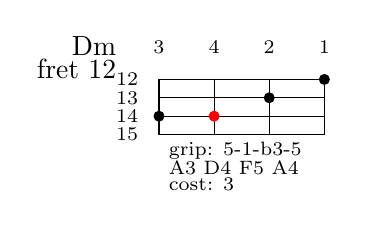
\begin{tikzpicture}[x=0.70cm,y=0.70cm]
\node[anchor=east] at (-0.6,1.6) {Dm};
\node[anchor=east] at (-0.6,1.2) {fret 12};
\draw (0.0,0.000) -- (0.0,1);
\draw (1.0,0.000) -- (1.0,1);
\draw (2.0,0.000) -- (2.0,1);
\draw (3.0,0.000) -- (3.0,1);
\draw (0.0,1.000) -- (3.0,1.000);
\node[anchor=east] at (-0.20,1.000) {\scriptsize 12};
\draw (0.0,0.667) -- (3.0,0.667);
\node[anchor=east] at (-0.20,0.667) {\scriptsize 13};
\draw (0.0,0.333) -- (3.0,0.333);
\node[anchor=east] at (-0.20,0.333) {\scriptsize 14};
\draw (0.0,0.000) -- (3.0,0.000);
\node[anchor=east] at (-0.20,0.000) {\scriptsize 15};
\node at (0.0,1.583) {\scriptsize 3};
\node at (1.0,1.583) {\scriptsize 4};
\node at (2.0,1.583) {\scriptsize 2};
\node at (3.0,1.583) {\scriptsize 1};
\fill[black] (0.0,0.333) circle (0.10);
\fill[red] (1.0,0.333) circle (0.10);
\fill[black] (2.0,0.667) circle (0.10);
\fill[black] (3.0,1.000) circle (0.10);
\node[anchor=west] at (0.0,-0.3) {\scriptsize grip: 5-1-b3-5};
\node[anchor=west] at (0.0,-0.6) {\scriptsize A3 D4 F5 A4};
\node[anchor=west] at (0.0,-0.9) {\scriptsize cost: 3};
\end{tikzpicture}
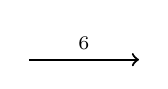
\begin{tikzpicture}[x=0.70cm,y=0.70cm]
\draw[->,thick] (0,0.5) -- (2.0,0.5);
\node at (1.0,0.8) {\scriptsize 6};
\end{tikzpicture}
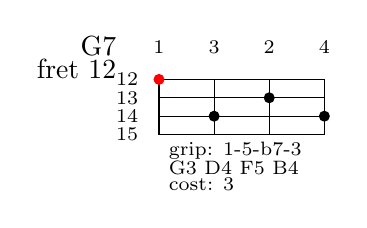
\begin{tikzpicture}[x=0.70cm,y=0.70cm]
\node[anchor=east] at (-0.6,1.6) {G7};
\node[anchor=east] at (-0.6,1.2) {fret 12};
\draw (0.0,0.000) -- (0.0,1);
\draw (1.0,0.000) -- (1.0,1);
\draw (2.0,0.000) -- (2.0,1);
\draw (3.0,0.000) -- (3.0,1);
\draw (0.0,1.000) -- (3.0,1.000);
\node[anchor=east] at (-0.20,1.000) {\scriptsize 12};
\draw (0.0,0.667) -- (3.0,0.667);
\node[anchor=east] at (-0.20,0.667) {\scriptsize 13};
\draw (0.0,0.333) -- (3.0,0.333);
\node[anchor=east] at (-0.20,0.333) {\scriptsize 14};
\draw (0.0,0.000) -- (3.0,0.000);
\node[anchor=east] at (-0.20,0.000) {\scriptsize 15};
\node at (0.0,1.583) {\scriptsize 1};
\node at (1.0,1.583) {\scriptsize 3};
\node at (2.0,1.583) {\scriptsize 2};
\node at (3.0,1.583) {\scriptsize 4};
\fill[red] (0.0,1.000) circle (0.10);
\fill[black] (1.0,0.333) circle (0.10);
\fill[black] (2.0,0.667) circle (0.10);
\fill[black] (3.0,0.333) circle (0.10);
\node[anchor=west] at (0.0,-0.3) {\scriptsize grip: 1-5-b7-3};
\node[anchor=west] at (0.0,-0.6) {\scriptsize G3 D4 F5 B4};
\node[anchor=west] at (0.0,-0.9) {\scriptsize cost: 3};
\end{tikzpicture}
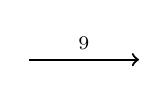
\begin{tikzpicture}[x=0.70cm,y=0.70cm]
\draw[->,thick] (0,0.5) -- (2.0,0.5);
\node at (1.0,0.8) {\scriptsize 9};
\end{tikzpicture}
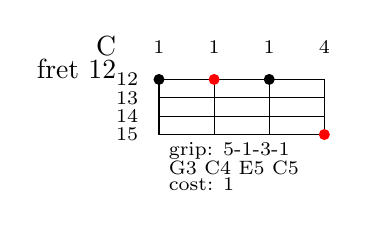
\begin{tikzpicture}[x=0.70cm,y=0.70cm]
\node[anchor=east] at (-0.6,1.6) {C};
\node[anchor=east] at (-0.6,1.2) {fret 12};
\draw (0.0,0.000) -- (0.0,1);
\draw (1.0,0.000) -- (1.0,1);
\draw (2.0,0.000) -- (2.0,1);
\draw (3.0,0.000) -- (3.0,1);
\draw (0.0,1.000) -- (3.0,1.000);
\node[anchor=east] at (-0.20,1.000) {\scriptsize 12};
\draw (0.0,0.667) -- (3.0,0.667);
\node[anchor=east] at (-0.20,0.667) {\scriptsize 13};
\draw (0.0,0.333) -- (3.0,0.333);
\node[anchor=east] at (-0.20,0.333) {\scriptsize 14};
\draw (0.0,0.000) -- (3.0,0.000);
\node[anchor=east] at (-0.20,0.000) {\scriptsize 15};
\node at (0.0,1.583) {\scriptsize 1};
\node at (1.0,1.583) {\scriptsize 1};
\node at (2.0,1.583) {\scriptsize 1};
\node at (3.0,1.583) {\scriptsize 4};
\fill[black] (0.0,1.000) circle (0.10);
\fill[red] (1.0,1.000) circle (0.10);
\fill[black] (2.0,1.000) circle (0.10);
\fill[red] (3.0,0.000) circle (0.10);
\node[anchor=west] at (0.0,-0.3) {\scriptsize grip: 5-1-3-1};
\node[anchor=west] at (0.0,-0.6) {\scriptsize G3 C4 E5 C5};
\node[anchor=west] at (0.0,-0.9) {\scriptsize cost: 1};
\end{tikzpicture}
\end{minipage} & \begin{minipage}[t]{0.09\linewidth}\raggedleft\textit{total cost: 22}\end{minipage}\\
\end{tabular}
\bigskip
\subsection*{F (ii-V-I)}
\begin{tabular}{@{}p{0.89\linewidth}r@{}}
\begin{minipage}[t]{0.89\linewidth}\raggedright
\textit{Gm C7 F}\\
\begin{tikzpicture}[x=0.70cm,y=0.70cm]
\node[anchor=east] at (-0.6,1.6) {Gm};
\node[anchor=east] at (-0.6,1.2) {fret 10};
\draw (0.0,0.000) -- (0.0,1);
\draw (1.0,0.000) -- (1.0,1);
\draw (2.0,0.000) -- (2.0,1);
\draw (3.0,0.000) -- (3.0,1);
\draw (0.0,1.000) -- (3.0,1.000);
\node[anchor=east] at (-0.20,1.000) {\scriptsize 10};
\draw (0.0,0.667) -- (3.0,0.667);
\node[anchor=east] at (-0.20,0.667) {\scriptsize 11};
\draw (0.0,0.333) -- (3.0,0.333);
\node[anchor=east] at (-0.20,0.333) {\scriptsize 12};
\draw (0.0,0.000) -- (3.0,0.000);
\node[anchor=east] at (-0.20,0.000) {\scriptsize 13};
\node at (0.0,1.583) {\scriptsize 3};
\node at (1.0,1.583) {\scriptsize 1};
\node at (2.0,1.583) {\scriptsize 1};
\node at (3.0,1.583) {\scriptsize 1};
\fill[red] (0.0,0.333) circle (0.10);
\fill[black] (1.0,1.000) circle (0.10);
\fill[black] (2.0,1.000) circle (0.10);
\fill[red] (3.0,1.000) circle (0.10);
\node[anchor=west] at (0.0,-0.3) {\scriptsize grip: 1-b3-5-1};
\node[anchor=west] at (0.0,-0.6) {\scriptsize G3 B♭3 D5 G4};
\node[anchor=west] at (0.0,-0.9) {\scriptsize cost: 0};
\end{tikzpicture}
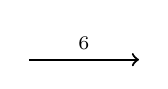
\begin{tikzpicture}[x=0.70cm,y=0.70cm]
\draw[->,thick] (0,0.5) -- (2.0,0.5);
\node at (1.0,0.8) {\scriptsize 6};
\end{tikzpicture}
\begin{tikzpicture}[x=0.70cm,y=0.70cm]
\node[anchor=east] at (-0.6,1.6) {C7};
\node[anchor=east] at (-0.6,1.2) {fret 8};
\draw (0.0,0.000) -- (0.0,1);
\draw (1.0,0.000) -- (1.0,1);
\draw (2.0,0.000) -- (2.0,1);
\draw (3.0,0.000) -- (3.0,1);
\draw (0.0,1.000) -- (3.0,1.000);
\node[anchor=east] at (-0.20,1.000) {\scriptsize 8};
\draw (0.0,0.667) -- (3.0,0.667);
\node[anchor=east] at (-0.20,0.667) {\scriptsize 9};
\draw (0.0,0.333) -- (3.0,0.333);
\node[anchor=east] at (-0.20,0.333) {\scriptsize 10};
\draw (0.0,0.000) -- (3.0,0.000);
\node[anchor=east] at (-0.20,0.000) {\scriptsize 11};
\node at (0.0,1.583) {\scriptsize 2};
\node at (1.0,1.583) {\scriptsize 3};
\node at (2.0,1.583) {\scriptsize 1};
\node at (3.0,1.583) {\scriptsize 4};
\fill[black] (0.0,0.667) circle (0.10);
\fill[black] (1.0,0.333) circle (0.10);
\fill[red] (2.0,1.000) circle (0.10);
\fill[black] (3.0,0.333) circle (0.10);
\node[anchor=west] at (0.0,-0.3) {\scriptsize grip: 3-b7-1-5};
\node[anchor=west] at (0.0,-0.6) {\scriptsize E3 B♭3 C5 G4};
\node[anchor=west] at (0.0,-0.9) {\scriptsize cost: 3};
\end{tikzpicture}
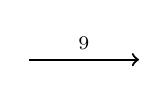
\begin{tikzpicture}[x=0.70cm,y=0.70cm]
\draw[->,thick] (0,0.5) -- (2.0,0.5);
\node at (1.0,0.8) {\scriptsize 9};
\end{tikzpicture}
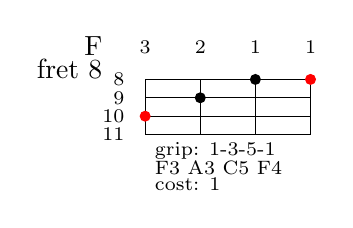
\begin{tikzpicture}[x=0.70cm,y=0.70cm]
\node[anchor=east] at (-0.6,1.6) {F};
\node[anchor=east] at (-0.6,1.2) {fret 8};
\draw (0.0,0.000) -- (0.0,1);
\draw (1.0,0.000) -- (1.0,1);
\draw (2.0,0.000) -- (2.0,1);
\draw (3.0,0.000) -- (3.0,1);
\draw (0.0,1.000) -- (3.0,1.000);
\node[anchor=east] at (-0.20,1.000) {\scriptsize 8};
\draw (0.0,0.667) -- (3.0,0.667);
\node[anchor=east] at (-0.20,0.667) {\scriptsize 9};
\draw (0.0,0.333) -- (3.0,0.333);
\node[anchor=east] at (-0.20,0.333) {\scriptsize 10};
\draw (0.0,0.000) -- (3.0,0.000);
\node[anchor=east] at (-0.20,0.000) {\scriptsize 11};
\node at (0.0,1.583) {\scriptsize 3};
\node at (1.0,1.583) {\scriptsize 2};
\node at (2.0,1.583) {\scriptsize 1};
\node at (3.0,1.583) {\scriptsize 1};
\fill[red] (0.0,0.333) circle (0.10);
\fill[black] (1.0,0.667) circle (0.10);
\fill[black] (2.0,1.000) circle (0.10);
\fill[red] (3.0,1.000) circle (0.10);
\node[anchor=west] at (0.0,-0.3) {\scriptsize grip: 1-3-5-1};
\node[anchor=west] at (0.0,-0.6) {\scriptsize F3 A3 C5 F4};
\node[anchor=west] at (0.0,-0.9) {\scriptsize cost: 1};
\end{tikzpicture}
\end{minipage} & \begin{minipage}[t]{0.09\linewidth}\raggedleft\textit{total cost: 19}\end{minipage}\\
\end{tabular}
\bigskip
\subsection*{Bb (ii-V-I)}
\begin{tabular}{@{}p{0.89\linewidth}r@{}}
\begin{minipage}[t]{0.89\linewidth}\raggedright
\textit{Cm F7 B♭}\\
\begin{tikzpicture}[x=0.70cm,y=0.70cm]
\node[anchor=east] at (-0.6,1.6) {Cm};
\node[anchor=east] at (-0.6,1.2) {fret 10};
\draw (0.0,0.000) -- (0.0,1);
\draw (1.0,0.000) -- (1.0,1);
\draw (2.0,0.000) -- (2.0,1);
\draw (3.0,0.000) -- (3.0,1);
\draw (0.0,1.000) -- (3.0,1.000);
\node[anchor=east] at (-0.20,1.000) {\scriptsize 10};
\draw (0.0,0.667) -- (3.0,0.667);
\node[anchor=east] at (-0.20,0.667) {\scriptsize 11};
\draw (0.0,0.333) -- (3.0,0.333);
\node[anchor=east] at (-0.20,0.333) {\scriptsize 12};
\draw (0.0,0.000) -- (3.0,0.000);
\node[anchor=east] at (-0.20,0.000) {\scriptsize 13};
\node at (0.0,1.583) {\scriptsize 3};
\node at (1.0,1.583) {\scriptsize 4};
\node at (2.0,1.583) {\scriptsize 2};
\node at (3.0,1.583) {\scriptsize 1};
\fill[black] (0.0,0.333) circle (0.10);
\fill[red] (1.0,0.333) circle (0.10);
\fill[black] (2.0,0.667) circle (0.10);
\fill[black] (3.0,1.000) circle (0.10);
\node[anchor=west] at (0.0,-0.3) {\scriptsize grip: 5-1-b3-5};
\node[anchor=west] at (0.0,-0.6) {\scriptsize G3 C4 E♭5 G4};
\node[anchor=west] at (0.0,-0.9) {\scriptsize cost: 3};
\end{tikzpicture}
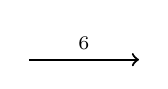
\begin{tikzpicture}[x=0.70cm,y=0.70cm]
\draw[->,thick] (0,0.5) -- (2.0,0.5);
\node at (1.0,0.8) {\scriptsize 6};
\end{tikzpicture}
\begin{tikzpicture}[x=0.70cm,y=0.70cm]
\node[anchor=east] at (-0.6,1.6) {F7};
\node[anchor=east] at (-0.6,1.2) {fret 10};
\draw (0.0,0.000) -- (0.0,1);
\draw (1.0,0.000) -- (1.0,1);
\draw (2.0,0.000) -- (2.0,1);
\draw (3.0,0.000) -- (3.0,1);
\draw (0.0,1.000) -- (3.0,1.000);
\node[anchor=east] at (-0.20,1.000) {\scriptsize 10};
\draw (0.0,0.667) -- (3.0,0.667);
\node[anchor=east] at (-0.20,0.667) {\scriptsize 11};
\draw (0.0,0.333) -- (3.0,0.333);
\node[anchor=east] at (-0.20,0.333) {\scriptsize 12};
\draw (0.0,0.000) -- (3.0,0.000);
\node[anchor=east] at (-0.20,0.000) {\scriptsize 13};
\node at (0.0,1.583) {\scriptsize 1};
\node at (1.0,1.583) {\scriptsize 3};
\node at (2.0,1.583) {\scriptsize 2};
\node at (3.0,1.583) {\scriptsize 4};
\fill[red] (0.0,1.000) circle (0.10);
\fill[black] (1.0,0.333) circle (0.10);
\fill[black] (2.0,0.667) circle (0.10);
\fill[black] (3.0,0.333) circle (0.10);
\node[anchor=west] at (0.0,-0.3) {\scriptsize grip: 1-5-b7-3};
\node[anchor=west] at (0.0,-0.6) {\scriptsize F3 C4 E♭5 A4};
\node[anchor=west] at (0.0,-0.9) {\scriptsize cost: 3};
\end{tikzpicture}
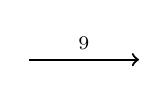
\begin{tikzpicture}[x=0.70cm,y=0.70cm]
\draw[->,thick] (0,0.5) -- (2.0,0.5);
\node at (1.0,0.8) {\scriptsize 9};
\end{tikzpicture}
\begin{tikzpicture}[x=0.70cm,y=0.70cm]
\node[anchor=east] at (-0.6,1.6) {B♭};
\node[anchor=east] at (-0.6,1.2) {fret 10};
\draw (0.0,0.000) -- (0.0,1);
\draw (1.0,0.000) -- (1.0,1);
\draw (2.0,0.000) -- (2.0,1);
\draw (3.0,0.000) -- (3.0,1);
\draw (0.0,1.000) -- (3.0,1.000);
\node[anchor=east] at (-0.20,1.000) {\scriptsize 10};
\draw (0.0,0.667) -- (3.0,0.667);
\node[anchor=east] at (-0.20,0.667) {\scriptsize 11};
\draw (0.0,0.333) -- (3.0,0.333);
\node[anchor=east] at (-0.20,0.333) {\scriptsize 12};
\draw (0.0,0.000) -- (3.0,0.000);
\node[anchor=east] at (-0.20,0.000) {\scriptsize 13};
\node at (0.0,1.583) {\scriptsize 1};
\node at (1.0,1.583) {\scriptsize 1};
\node at (2.0,1.583) {\scriptsize 1};
\node at (3.0,1.583) {\scriptsize 4};
\fill[black] (0.0,1.000) circle (0.10);
\fill[red] (1.0,1.000) circle (0.10);
\fill[black] (2.0,1.000) circle (0.10);
\fill[red] (3.0,0.000) circle (0.10);
\node[anchor=west] at (0.0,-0.3) {\scriptsize grip: 5-1-3-1};
\node[anchor=west] at (0.0,-0.6) {\scriptsize F3 B♭3 D5 B♭4};
\node[anchor=west] at (0.0,-0.9) {\scriptsize cost: 1};
\end{tikzpicture}
\end{minipage} & \begin{minipage}[t]{0.09\linewidth}\raggedleft\textit{total cost: 22}\end{minipage}\\
\end{tabular}
\bigskip
\subsection*{Eb (ii-V-I)}
\begin{tabular}{@{}p{0.89\linewidth}r@{}}
\begin{minipage}[t]{0.89\linewidth}\raggedright
\textit{Fm B♭7 E♭}\\
\begin{tikzpicture}[x=0.70cm,y=0.70cm]
\node[anchor=east] at (-0.6,1.6) {Fm};
\node[anchor=east] at (-0.6,1.2) {fret 8};
\draw (0.0,0.000) -- (0.0,1);
\draw (1.0,0.000) -- (1.0,1);
\draw (2.0,0.000) -- (2.0,1);
\draw (3.0,0.000) -- (3.0,1);
\draw (0.0,1.000) -- (3.0,1.000);
\node[anchor=east] at (-0.20,1.000) {\scriptsize 8};
\draw (0.0,0.667) -- (3.0,0.667);
\node[anchor=east] at (-0.20,0.667) {\scriptsize 9};
\draw (0.0,0.333) -- (3.0,0.333);
\node[anchor=east] at (-0.20,0.333) {\scriptsize 10};
\draw (0.0,0.000) -- (3.0,0.000);
\node[anchor=east] at (-0.20,0.000) {\scriptsize 11};
\node at (0.0,1.583) {\scriptsize 3};
\node at (1.0,1.583) {\scriptsize 1};
\node at (2.0,1.583) {\scriptsize 1};
\node at (3.0,1.583) {\scriptsize 1};
\fill[red] (0.0,0.333) circle (0.10);
\fill[black] (1.0,1.000) circle (0.10);
\fill[black] (2.0,1.000) circle (0.10);
\fill[red] (3.0,1.000) circle (0.10);
\node[anchor=west] at (0.0,-0.3) {\scriptsize grip: 1-b3-5-1};
\node[anchor=west] at (0.0,-0.6) {\scriptsize F3 A♭3 C5 F4};
\node[anchor=west] at (0.0,-0.9) {\scriptsize cost: 0};
\end{tikzpicture}
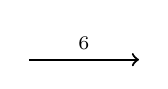
\begin{tikzpicture}[x=0.70cm,y=0.70cm]
\draw[->,thick] (0,0.5) -- (2.0,0.5);
\node at (1.0,0.8) {\scriptsize 6};
\end{tikzpicture}
\begin{tikzpicture}[x=0.70cm,y=0.70cm]
\node[anchor=east] at (-0.6,1.6) {B♭7};
\node[anchor=east] at (-0.6,1.2) {fret 6};
\draw (0.0,0.000) -- (0.0,1);
\draw (1.0,0.000) -- (1.0,1);
\draw (2.0,0.000) -- (2.0,1);
\draw (3.0,0.000) -- (3.0,1);
\draw (0.0,1.000) -- (3.0,1.000);
\node[anchor=east] at (-0.20,1.000) {\scriptsize 6};
\draw (0.0,0.667) -- (3.0,0.667);
\node[anchor=east] at (-0.20,0.667) {\scriptsize 7};
\draw (0.0,0.333) -- (3.0,0.333);
\node[anchor=east] at (-0.20,0.333) {\scriptsize 8};
\draw (0.0,0.000) -- (3.0,0.000);
\node[anchor=east] at (-0.20,0.000) {\scriptsize 9};
\node at (0.0,1.583) {\scriptsize 2};
\node at (1.0,1.583) {\scriptsize 3};
\node at (2.0,1.583) {\scriptsize 1};
\node at (3.0,1.583) {\scriptsize 4};
\fill[black] (0.0,0.667) circle (0.10);
\fill[black] (1.0,0.333) circle (0.10);
\fill[red] (2.0,1.000) circle (0.10);
\fill[black] (3.0,0.333) circle (0.10);
\node[anchor=west] at (0.0,-0.3) {\scriptsize grip: 3-b7-1-5};
\node[anchor=west] at (0.0,-0.6) {\scriptsize D3 A♭3 B♭4 F4};
\node[anchor=west] at (0.0,-0.9) {\scriptsize cost: 3};
\end{tikzpicture}
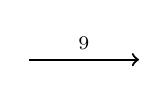
\begin{tikzpicture}[x=0.70cm,y=0.70cm]
\draw[->,thick] (0,0.5) -- (2.0,0.5);
\node at (1.0,0.8) {\scriptsize 9};
\end{tikzpicture}
\begin{tikzpicture}[x=0.70cm,y=0.70cm]
\node[anchor=east] at (-0.6,1.6) {E♭};
\node[anchor=east] at (-0.6,1.2) {fret 6};
\draw (0.0,0.000) -- (0.0,1);
\draw (1.0,0.000) -- (1.0,1);
\draw (2.0,0.000) -- (2.0,1);
\draw (3.0,0.000) -- (3.0,1);
\draw (0.0,1.000) -- (3.0,1.000);
\node[anchor=east] at (-0.20,1.000) {\scriptsize 6};
\draw (0.0,0.667) -- (3.0,0.667);
\node[anchor=east] at (-0.20,0.667) {\scriptsize 7};
\draw (0.0,0.333) -- (3.0,0.333);
\node[anchor=east] at (-0.20,0.333) {\scriptsize 8};
\draw (0.0,0.000) -- (3.0,0.000);
\node[anchor=east] at (-0.20,0.000) {\scriptsize 9};
\node at (0.0,1.583) {\scriptsize 3};
\node at (1.0,1.583) {\scriptsize 2};
\node at (2.0,1.583) {\scriptsize 1};
\node at (3.0,1.583) {\scriptsize 1};
\fill[red] (0.0,0.333) circle (0.10);
\fill[black] (1.0,0.667) circle (0.10);
\fill[black] (2.0,1.000) circle (0.10);
\fill[red] (3.0,1.000) circle (0.10);
\node[anchor=west] at (0.0,-0.3) {\scriptsize grip: 1-3-5-1};
\node[anchor=west] at (0.0,-0.6) {\scriptsize E♭3 G3 B♭4 E♭4};
\node[anchor=west] at (0.0,-0.9) {\scriptsize cost: 1};
\end{tikzpicture}
\end{minipage} & \begin{minipage}[t]{0.09\linewidth}\raggedleft\textit{total cost: 19}\end{minipage}\\
\end{tabular}
\bigskip
\subsection*{Ab (ii-V-I)}
\begin{tabular}{@{}p{0.89\linewidth}r@{}}
\begin{minipage}[t]{0.89\linewidth}\raggedright
\textit{B♭m E♭7 A♭}\\
\begin{tikzpicture}[x=0.70cm,y=0.70cm]
\node[anchor=east] at (-0.6,1.6) {B♭m};
\node[anchor=east] at (-0.6,1.2) {fret 8};
\draw (0.0,0.000) -- (0.0,1);
\draw (1.0,0.000) -- (1.0,1);
\draw (2.0,0.000) -- (2.0,1);
\draw (3.0,0.000) -- (3.0,1);
\draw (0.0,1.000) -- (3.0,1.000);
\node[anchor=east] at (-0.20,1.000) {\scriptsize 8};
\draw (0.0,0.667) -- (3.0,0.667);
\node[anchor=east] at (-0.20,0.667) {\scriptsize 9};
\draw (0.0,0.333) -- (3.0,0.333);
\node[anchor=east] at (-0.20,0.333) {\scriptsize 10};
\draw (0.0,0.000) -- (3.0,0.000);
\node[anchor=east] at (-0.20,0.000) {\scriptsize 11};
\node at (0.0,1.583) {\scriptsize 3};
\node at (1.0,1.583) {\scriptsize 4};
\node at (2.0,1.583) {\scriptsize 2};
\node at (3.0,1.583) {\scriptsize 1};
\fill[black] (0.0,0.333) circle (0.10);
\fill[red] (1.0,0.333) circle (0.10);
\fill[black] (2.0,0.667) circle (0.10);
\fill[black] (3.0,1.000) circle (0.10);
\node[anchor=west] at (0.0,-0.3) {\scriptsize grip: 5-1-b3-5};
\node[anchor=west] at (0.0,-0.6) {\scriptsize F3 B♭3 C♯5 F4};
\node[anchor=west] at (0.0,-0.9) {\scriptsize cost: 3};
\end{tikzpicture}
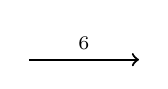
\begin{tikzpicture}[x=0.70cm,y=0.70cm]
\draw[->,thick] (0,0.5) -- (2.0,0.5);
\node at (1.0,0.8) {\scriptsize 6};
\end{tikzpicture}
\begin{tikzpicture}[x=0.70cm,y=0.70cm]
\node[anchor=east] at (-0.6,1.6) {E♭7};
\node[anchor=east] at (-0.6,1.2) {fret 8};
\draw (0.0,0.000) -- (0.0,1);
\draw (1.0,0.000) -- (1.0,1);
\draw (2.0,0.000) -- (2.0,1);
\draw (3.0,0.000) -- (3.0,1);
\draw (0.0,1.000) -- (3.0,1.000);
\node[anchor=east] at (-0.20,1.000) {\scriptsize 8};
\draw (0.0,0.667) -- (3.0,0.667);
\node[anchor=east] at (-0.20,0.667) {\scriptsize 9};
\draw (0.0,0.333) -- (3.0,0.333);
\node[anchor=east] at (-0.20,0.333) {\scriptsize 10};
\draw (0.0,0.000) -- (3.0,0.000);
\node[anchor=east] at (-0.20,0.000) {\scriptsize 11};
\node at (0.0,1.583) {\scriptsize 1};
\node at (1.0,1.583) {\scriptsize 3};
\node at (2.0,1.583) {\scriptsize 2};
\node at (3.0,1.583) {\scriptsize 4};
\fill[red] (0.0,1.000) circle (0.10);
\fill[black] (1.0,0.333) circle (0.10);
\fill[black] (2.0,0.667) circle (0.10);
\fill[black] (3.0,0.333) circle (0.10);
\node[anchor=west] at (0.0,-0.3) {\scriptsize grip: 1-5-b7-3};
\node[anchor=west] at (0.0,-0.6) {\scriptsize E♭3 B♭3 C♯5 G4};
\node[anchor=west] at (0.0,-0.9) {\scriptsize cost: 3};
\end{tikzpicture}
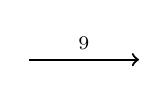
\begin{tikzpicture}[x=0.70cm,y=0.70cm]
\draw[->,thick] (0,0.5) -- (2.0,0.5);
\node at (1.0,0.8) {\scriptsize 9};
\end{tikzpicture}
\begin{tikzpicture}[x=0.70cm,y=0.70cm]
\node[anchor=east] at (-0.6,1.6) {A♭};
\node[anchor=east] at (-0.6,1.2) {fret 8};
\draw (0.0,0.000) -- (0.0,1);
\draw (1.0,0.000) -- (1.0,1);
\draw (2.0,0.000) -- (2.0,1);
\draw (3.0,0.000) -- (3.0,1);
\draw (0.0,1.000) -- (3.0,1.000);
\node[anchor=east] at (-0.20,1.000) {\scriptsize 8};
\draw (0.0,0.667) -- (3.0,0.667);
\node[anchor=east] at (-0.20,0.667) {\scriptsize 9};
\draw (0.0,0.333) -- (3.0,0.333);
\node[anchor=east] at (-0.20,0.333) {\scriptsize 10};
\draw (0.0,0.000) -- (3.0,0.000);
\node[anchor=east] at (-0.20,0.000) {\scriptsize 11};
\node at (0.0,1.583) {\scriptsize 1};
\node at (1.0,1.583) {\scriptsize 1};
\node at (2.0,1.583) {\scriptsize 1};
\node at (3.0,1.583) {\scriptsize 4};
\fill[black] (0.0,1.000) circle (0.10);
\fill[red] (1.0,1.000) circle (0.10);
\fill[black] (2.0,1.000) circle (0.10);
\fill[red] (3.0,0.000) circle (0.10);
\node[anchor=west] at (0.0,-0.3) {\scriptsize grip: 5-1-3-1};
\node[anchor=west] at (0.0,-0.6) {\scriptsize E♭3 A♭3 C5 A♭4};
\node[anchor=west] at (0.0,-0.9) {\scriptsize cost: 1};
\end{tikzpicture}
\end{minipage} & \begin{minipage}[t]{0.09\linewidth}\raggedleft\textit{total cost: 22}\end{minipage}\\
\end{tabular}
\bigskip
\subsection*{Db (ii-V-I)}
\begin{tabular}{@{}p{0.89\linewidth}r@{}}
\begin{minipage}[t]{0.89\linewidth}\raggedright
\textit{E♭m A♭7 C♯}\\
\begin{tikzpicture}[x=0.70cm,y=0.70cm]
\node[anchor=east] at (-0.6,1.6) {E♭m};
\node[anchor=east] at (-0.6,1.2) {fret 9};
\draw (0.0,0.000) -- (0.0,1);
\draw (1.0,0.000) -- (1.0,1);
\draw (2.0,0.000) -- (2.0,1);
\draw (3.0,0.000) -- (3.0,1);
\draw (0.0,1.000) -- (3.0,1.000);
\node[anchor=east] at (-0.20,1.000) {\scriptsize 9};
\draw (0.0,0.667) -- (3.0,0.667);
\node[anchor=east] at (-0.20,0.667) {\scriptsize 10};
\draw (0.0,0.333) -- (3.0,0.333);
\node[anchor=east] at (-0.20,0.333) {\scriptsize 11};
\draw (0.0,0.000) -- (3.0,0.000);
\node[anchor=east] at (-0.20,0.000) {\scriptsize 12};
\node at (0.0,1.583) {\scriptsize 3};
\node at (1.0,1.583) {\scriptsize 2};
\node at (2.0,1.583) {\scriptsize 4};
\node at (3.0,1.583) {\scriptsize 1};
\fill[black] (0.0,0.333) circle (0.10);
\fill[black] (1.0,0.667) circle (0.10);
\fill[red] (2.0,0.333) circle (0.10);
\fill[black] (3.0,1.000) circle (0.10);
\node[anchor=west] at (0.0,-0.3) {\scriptsize grip: b3-5-1-b3};
\node[anchor=west] at (0.0,-0.6) {\scriptsize F♯3 B♭3 E♭5 F♯4};
\node[anchor=west] at (0.0,-0.9) {\scriptsize cost: 3};
\end{tikzpicture}
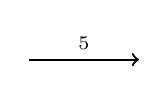
\begin{tikzpicture}[x=0.70cm,y=0.70cm]
\draw[->,thick] (0,0.5) -- (2.0,0.5);
\node at (1.0,0.8) {\scriptsize 5};
\end{tikzpicture}
\begin{tikzpicture}[x=0.70cm,y=0.70cm]
\node[anchor=east] at (-0.6,1.6) {A♭7};
\node[anchor=east] at (-0.6,1.2) {fret 11};
\draw (0.0,0.000) -- (0.0,1);
\draw (1.0,0.000) -- (1.0,1);
\draw (2.0,0.000) -- (2.0,1);
\draw (3.0,0.000) -- (3.0,1);
\draw (0.0,1.000) -- (3.0,1.000);
\node[anchor=east] at (-0.20,1.000) {\scriptsize 11};
\draw (0.0,0.667) -- (3.0,0.667);
\node[anchor=east] at (-0.20,0.667) {\scriptsize 12};
\draw (0.0,0.333) -- (3.0,0.333);
\node[anchor=east] at (-0.20,0.333) {\scriptsize 13};
\draw (0.0,0.000) -- (3.0,0.000);
\node[anchor=east] at (-0.20,0.000) {\scriptsize 14};
\node at (0.0,1.583) {\scriptsize 1};
\node at (1.0,1.583) {\scriptsize 2};
\node at (2.0,1.583) {\scriptsize 1};
\node at (3.0,1.583) {\scriptsize 1};
\fill[black] (0.0,1.000) circle (0.10);
\fill[black] (1.0,0.667) circle (0.10);
\fill[black] (2.0,1.000) circle (0.10);
\fill[red] (3.0,1.000) circle (0.10);
\node[anchor=west] at (0.0,-0.3) {\scriptsize grip: b7-3-5-1};
\node[anchor=west] at (0.0,-0.6) {\scriptsize F♯3 C4 E♭5 A♭4};
\node[anchor=west] at (0.0,-0.9) {\scriptsize cost: 0};
\end{tikzpicture}
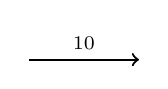
\begin{tikzpicture}[x=0.70cm,y=0.70cm]
\draw[->,thick] (0,0.5) -- (2.0,0.5);
\node at (1.0,0.8) {\scriptsize 10};
\end{tikzpicture}
\begin{tikzpicture}[x=0.70cm,y=0.70cm]
\node[anchor=east] at (-0.6,1.6) {C♯};
\node[anchor=east] at (-0.6,1.2) {fret 11};
\draw (0.0,0.000) -- (0.0,1);
\draw (1.0,0.000) -- (1.0,1);
\draw (2.0,0.000) -- (2.0,1);
\draw (3.0,0.000) -- (3.0,1);
\draw (0.0,1.000) -- (3.0,1.000);
\node[anchor=east] at (-0.20,1.000) {\scriptsize 11};
\draw (0.0,0.667) -- (3.0,0.667);
\node[anchor=east] at (-0.20,0.667) {\scriptsize 12};
\draw (0.0,0.333) -- (3.0,0.333);
\node[anchor=east] at (-0.20,0.333) {\scriptsize 13};
\draw (0.0,0.000) -- (3.0,0.000);
\node[anchor=east] at (-0.20,0.000) {\scriptsize 14};
\node at (0.0,1.583) {\scriptsize 2};
\node at (1.0,1.583) {\scriptsize 3};
\node at (2.0,1.583) {\scriptsize 4};
\node at (3.0,1.583) {\scriptsize 1};
\fill[black] (0.0,0.333) circle (0.10);
\fill[red] (1.0,0.333) circle (0.10);
\fill[black] (2.0,0.333) circle (0.10);
\fill[black] (3.0,1.000) circle (0.10);
\node[anchor=west] at (0.0,-0.3) {\scriptsize grip: 5-1-3-5};
\node[anchor=west] at (0.0,-0.6) {\scriptsize A♭3 C♯4 F5 A♭4};
\node[anchor=west] at (0.0,-0.9) {\scriptsize cost: 4};
\end{tikzpicture}
\end{minipage} & \begin{minipage}[t]{0.09\linewidth}\raggedleft\textit{total cost: 22}\end{minipage}\\
\end{tabular}
\bigskip
\subsection*{Gb (ii-V-I)}
\begin{tabular}{@{}p{0.89\linewidth}r@{}}
\begin{minipage}[t]{0.89\linewidth}\raggedright
\textit{A♭m C♯7 F♯}\\
\begin{tikzpicture}[x=0.70cm,y=0.70cm]
\node[anchor=east] at (-0.6,1.6) {A♭m};
\node[anchor=east] at (-0.6,1.2) {fret 11};
\draw (0.0,0.000) -- (0.0,1);
\draw (1.0,0.000) -- (1.0,1);
\draw (2.0,0.000) -- (2.0,1);
\draw (3.0,0.000) -- (3.0,1);
\draw (0.0,1.000) -- (3.0,1.000);
\node[anchor=east] at (-0.20,1.000) {\scriptsize 11};
\draw (0.0,0.667) -- (3.0,0.667);
\node[anchor=east] at (-0.20,0.667) {\scriptsize 12};
\draw (0.0,0.333) -- (3.0,0.333);
\node[anchor=east] at (-0.20,0.333) {\scriptsize 13};
\draw (0.0,0.000) -- (3.0,0.000);
\node[anchor=east] at (-0.20,0.000) {\scriptsize 14};
\node at (0.0,1.583) {\scriptsize 3};
\node at (1.0,1.583) {\scriptsize 1};
\node at (2.0,1.583) {\scriptsize 1};
\node at (3.0,1.583) {\scriptsize 1};
\fill[red] (0.0,0.333) circle (0.10);
\fill[black] (1.0,1.000) circle (0.10);
\fill[black] (2.0,1.000) circle (0.10);
\fill[red] (3.0,1.000) circle (0.10);
\node[anchor=west] at (0.0,-0.3) {\scriptsize grip: 1-b3-5-1};
\node[anchor=west] at (0.0,-0.6) {\scriptsize A♭3 B3 E♭5 A♭4};
\node[anchor=west] at (0.0,-0.9) {\scriptsize cost: 0};
\end{tikzpicture}
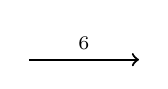
\begin{tikzpicture}[x=0.70cm,y=0.70cm]
\draw[->,thick] (0,0.5) -- (2.0,0.5);
\node at (1.0,0.8) {\scriptsize 6};
\end{tikzpicture}
\begin{tikzpicture}[x=0.70cm,y=0.70cm]
\node[anchor=east] at (-0.6,1.6) {C♯7};
\node[anchor=east] at (-0.6,1.2) {fret 9};
\draw (0.0,0.000) -- (0.0,1);
\draw (1.0,0.000) -- (1.0,1);
\draw (2.0,0.000) -- (2.0,1);
\draw (3.0,0.000) -- (3.0,1);
\draw (0.0,1.000) -- (3.0,1.000);
\node[anchor=east] at (-0.20,1.000) {\scriptsize 9};
\draw (0.0,0.667) -- (3.0,0.667);
\node[anchor=east] at (-0.20,0.667) {\scriptsize 10};
\draw (0.0,0.333) -- (3.0,0.333);
\node[anchor=east] at (-0.20,0.333) {\scriptsize 11};
\draw (0.0,0.000) -- (3.0,0.000);
\node[anchor=east] at (-0.20,0.000) {\scriptsize 12};
\node at (0.0,1.583) {\scriptsize 2};
\node at (1.0,1.583) {\scriptsize 3};
\node at (2.0,1.583) {\scriptsize 1};
\node at (3.0,1.583) {\scriptsize 4};
\fill[black] (0.0,0.667) circle (0.10);
\fill[black] (1.0,0.333) circle (0.10);
\fill[red] (2.0,1.000) circle (0.10);
\fill[black] (3.0,0.333) circle (0.10);
\node[anchor=west] at (0.0,-0.3) {\scriptsize grip: 3-b7-1-5};
\node[anchor=west] at (0.0,-0.6) {\scriptsize F3 B3 C♯5 A♭4};
\node[anchor=west] at (0.0,-0.9) {\scriptsize cost: 3};
\end{tikzpicture}
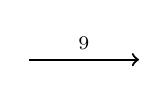
\begin{tikzpicture}[x=0.70cm,y=0.70cm]
\draw[->,thick] (0,0.5) -- (2.0,0.5);
\node at (1.0,0.8) {\scriptsize 9};
\end{tikzpicture}
\begin{tikzpicture}[x=0.70cm,y=0.70cm]
\node[anchor=east] at (-0.6,1.6) {F♯};
\node[anchor=east] at (-0.6,1.2) {fret 9};
\draw (0.0,0.000) -- (0.0,1);
\draw (1.0,0.000) -- (1.0,1);
\draw (2.0,0.000) -- (2.0,1);
\draw (3.0,0.000) -- (3.0,1);
\draw (0.0,1.000) -- (3.0,1.000);
\node[anchor=east] at (-0.20,1.000) {\scriptsize 9};
\draw (0.0,0.667) -- (3.0,0.667);
\node[anchor=east] at (-0.20,0.667) {\scriptsize 10};
\draw (0.0,0.333) -- (3.0,0.333);
\node[anchor=east] at (-0.20,0.333) {\scriptsize 11};
\draw (0.0,0.000) -- (3.0,0.000);
\node[anchor=east] at (-0.20,0.000) {\scriptsize 12};
\node at (0.0,1.583) {\scriptsize 3};
\node at (1.0,1.583) {\scriptsize 2};
\node at (2.0,1.583) {\scriptsize 1};
\node at (3.0,1.583) {\scriptsize 1};
\fill[red] (0.0,0.333) circle (0.10);
\fill[black] (1.0,0.667) circle (0.10);
\fill[black] (2.0,1.000) circle (0.10);
\fill[red] (3.0,1.000) circle (0.10);
\node[anchor=west] at (0.0,-0.3) {\scriptsize grip: 1-3-5-1};
\node[anchor=west] at (0.0,-0.6) {\scriptsize F♯3 B♭3 C♯5 F♯4};
\node[anchor=west] at (0.0,-0.9) {\scriptsize cost: 1};
\end{tikzpicture}
\end{minipage} & \begin{minipage}[t]{0.09\linewidth}\raggedleft\textit{total cost: 19}\end{minipage}\\
\end{tabular}
\bigskip
\subsection*{B (ii-V-I)}
\begin{tabular}{@{}p{0.89\linewidth}r@{}}
\begin{minipage}[t]{0.89\linewidth}\raggedright
\textit{C♯m F♯7 B}\\
\begin{tikzpicture}[x=0.70cm,y=0.70cm]
\node[anchor=east] at (-0.6,1.6) {C♯m};
\node[anchor=east] at (-0.6,1.2) {fret 11};
\draw (0.0,0.000) -- (0.0,1);
\draw (1.0,0.000) -- (1.0,1);
\draw (2.0,0.000) -- (2.0,1);
\draw (3.0,0.000) -- (3.0,1);
\draw (0.0,1.000) -- (3.0,1.000);
\node[anchor=east] at (-0.20,1.000) {\scriptsize 11};
\draw (0.0,0.667) -- (3.0,0.667);
\node[anchor=east] at (-0.20,0.667) {\scriptsize 12};
\draw (0.0,0.333) -- (3.0,0.333);
\node[anchor=east] at (-0.20,0.333) {\scriptsize 13};
\draw (0.0,0.000) -- (3.0,0.000);
\node[anchor=east] at (-0.20,0.000) {\scriptsize 14};
\node at (0.0,1.583) {\scriptsize 3};
\node at (1.0,1.583) {\scriptsize 4};
\node at (2.0,1.583) {\scriptsize 2};
\node at (3.0,1.583) {\scriptsize 1};
\fill[black] (0.0,0.333) circle (0.10);
\fill[red] (1.0,0.333) circle (0.10);
\fill[black] (2.0,0.667) circle (0.10);
\fill[black] (3.0,1.000) circle (0.10);
\node[anchor=west] at (0.0,-0.3) {\scriptsize grip: 5-1-b3-5};
\node[anchor=west] at (0.0,-0.6) {\scriptsize A♭3 C♯4 E5 A♭4};
\node[anchor=west] at (0.0,-0.9) {\scriptsize cost: 3};
\end{tikzpicture}
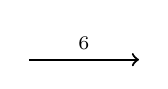
\begin{tikzpicture}[x=0.70cm,y=0.70cm]
\draw[->,thick] (0,0.5) -- (2.0,0.5);
\node at (1.0,0.8) {\scriptsize 6};
\end{tikzpicture}
\begin{tikzpicture}[x=0.70cm,y=0.70cm]
\node[anchor=east] at (-0.6,1.6) {F♯7};
\node[anchor=east] at (-0.6,1.2) {fret 11};
\draw (0.0,0.000) -- (0.0,1);
\draw (1.0,0.000) -- (1.0,1);
\draw (2.0,0.000) -- (2.0,1);
\draw (3.0,0.000) -- (3.0,1);
\draw (0.0,1.000) -- (3.0,1.000);
\node[anchor=east] at (-0.20,1.000) {\scriptsize 11};
\draw (0.0,0.667) -- (3.0,0.667);
\node[anchor=east] at (-0.20,0.667) {\scriptsize 12};
\draw (0.0,0.333) -- (3.0,0.333);
\node[anchor=east] at (-0.20,0.333) {\scriptsize 13};
\draw (0.0,0.000) -- (3.0,0.000);
\node[anchor=east] at (-0.20,0.000) {\scriptsize 14};
\node at (0.0,1.583) {\scriptsize 1};
\node at (1.0,1.583) {\scriptsize 3};
\node at (2.0,1.583) {\scriptsize 2};
\node at (3.0,1.583) {\scriptsize 4};
\fill[red] (0.0,1.000) circle (0.10);
\fill[black] (1.0,0.333) circle (0.10);
\fill[black] (2.0,0.667) circle (0.10);
\fill[black] (3.0,0.333) circle (0.10);
\node[anchor=west] at (0.0,-0.3) {\scriptsize grip: 1-5-b7-3};
\node[anchor=west] at (0.0,-0.6) {\scriptsize F♯3 C♯4 E5 B♭4};
\node[anchor=west] at (0.0,-0.9) {\scriptsize cost: 3};
\end{tikzpicture}
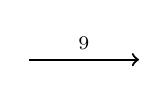
\begin{tikzpicture}[x=0.70cm,y=0.70cm]
\draw[->,thick] (0,0.5) -- (2.0,0.5);
\node at (1.0,0.8) {\scriptsize 9};
\end{tikzpicture}
\begin{tikzpicture}[x=0.70cm,y=0.70cm]
\node[anchor=east] at (-0.6,1.6) {B};
\node[anchor=east] at (-0.6,1.2) {fret 11};
\draw (0.0,0.000) -- (0.0,1);
\draw (1.0,0.000) -- (1.0,1);
\draw (2.0,0.000) -- (2.0,1);
\draw (3.0,0.000) -- (3.0,1);
\draw (0.0,1.000) -- (3.0,1.000);
\node[anchor=east] at (-0.20,1.000) {\scriptsize 11};
\draw (0.0,0.667) -- (3.0,0.667);
\node[anchor=east] at (-0.20,0.667) {\scriptsize 12};
\draw (0.0,0.333) -- (3.0,0.333);
\node[anchor=east] at (-0.20,0.333) {\scriptsize 13};
\draw (0.0,0.000) -- (3.0,0.000);
\node[anchor=east] at (-0.20,0.000) {\scriptsize 14};
\node at (0.0,1.583) {\scriptsize 1};
\node at (1.0,1.583) {\scriptsize 1};
\node at (2.0,1.583) {\scriptsize 1};
\node at (3.0,1.583) {\scriptsize 4};
\fill[black] (0.0,1.000) circle (0.10);
\fill[red] (1.0,1.000) circle (0.10);
\fill[black] (2.0,1.000) circle (0.10);
\fill[red] (3.0,0.000) circle (0.10);
\node[anchor=west] at (0.0,-0.3) {\scriptsize grip: 5-1-3-1};
\node[anchor=west] at (0.0,-0.6) {\scriptsize F♯3 B3 E♭5 B4};
\node[anchor=west] at (0.0,-0.9) {\scriptsize cost: 1};
\end{tikzpicture}
\end{minipage} & \begin{minipage}[t]{0.09\linewidth}\raggedleft\textit{total cost: 22}\end{minipage}\\
\end{tabular}
\bigskip
\subsection*{E (ii-V-I)}
\begin{tabular}{@{}p{0.89\linewidth}r@{}}
\begin{minipage}[t]{0.89\linewidth}\raggedright
\textit{F♯m B7 E}\\
\begin{tikzpicture}[x=0.70cm,y=0.70cm]
\node[anchor=east] at (-0.6,1.6) {F♯m};
\node[anchor=east] at (-0.6,1.2) {fret 9};
\draw (0.0,0.000) -- (0.0,1);
\draw (1.0,0.000) -- (1.0,1);
\draw (2.0,0.000) -- (2.0,1);
\draw (3.0,0.000) -- (3.0,1);
\draw (0.0,1.000) -- (3.0,1.000);
\node[anchor=east] at (-0.20,1.000) {\scriptsize 9};
\draw (0.0,0.667) -- (3.0,0.667);
\node[anchor=east] at (-0.20,0.667) {\scriptsize 10};
\draw (0.0,0.333) -- (3.0,0.333);
\node[anchor=east] at (-0.20,0.333) {\scriptsize 11};
\draw (0.0,0.000) -- (3.0,0.000);
\node[anchor=east] at (-0.20,0.000) {\scriptsize 12};
\node at (0.0,1.583) {\scriptsize 3};
\node at (1.0,1.583) {\scriptsize 1};
\node at (2.0,1.583) {\scriptsize 1};
\node at (3.0,1.583) {\scriptsize 1};
\fill[red] (0.0,0.333) circle (0.10);
\fill[black] (1.0,1.000) circle (0.10);
\fill[black] (2.0,1.000) circle (0.10);
\fill[red] (3.0,1.000) circle (0.10);
\node[anchor=west] at (0.0,-0.3) {\scriptsize grip: 1-b3-5-1};
\node[anchor=west] at (0.0,-0.6) {\scriptsize F♯3 A3 C♯5 F♯4};
\node[anchor=west] at (0.0,-0.9) {\scriptsize cost: 0};
\end{tikzpicture}
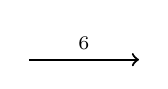
\begin{tikzpicture}[x=0.70cm,y=0.70cm]
\draw[->,thick] (0,0.5) -- (2.0,0.5);
\node at (1.0,0.8) {\scriptsize 6};
\end{tikzpicture}
\begin{tikzpicture}[x=0.70cm,y=0.70cm]
\node[anchor=east] at (-0.6,1.6) {B7};
\node[anchor=east] at (-0.6,1.2) {fret 7};
\draw (0.0,0.000) -- (0.0,1);
\draw (1.0,0.000) -- (1.0,1);
\draw (2.0,0.000) -- (2.0,1);
\draw (3.0,0.000) -- (3.0,1);
\draw (0.0,1.000) -- (3.0,1.000);
\node[anchor=east] at (-0.20,1.000) {\scriptsize 7};
\draw (0.0,0.667) -- (3.0,0.667);
\node[anchor=east] at (-0.20,0.667) {\scriptsize 8};
\draw (0.0,0.333) -- (3.0,0.333);
\node[anchor=east] at (-0.20,0.333) {\scriptsize 9};
\draw (0.0,0.000) -- (3.0,0.000);
\node[anchor=east] at (-0.20,0.000) {\scriptsize 10};
\node at (0.0,1.583) {\scriptsize 2};
\node at (1.0,1.583) {\scriptsize 3};
\node at (2.0,1.583) {\scriptsize 1};
\node at (3.0,1.583) {\scriptsize 4};
\fill[black] (0.0,0.667) circle (0.10);
\fill[black] (1.0,0.333) circle (0.10);
\fill[red] (2.0,1.000) circle (0.10);
\fill[black] (3.0,0.333) circle (0.10);
\node[anchor=west] at (0.0,-0.3) {\scriptsize grip: 3-b7-1-5};
\node[anchor=west] at (0.0,-0.6) {\scriptsize E♭3 A3 B4 F♯4};
\node[anchor=west] at (0.0,-0.9) {\scriptsize cost: 3};
\end{tikzpicture}
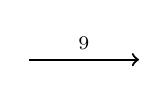
\begin{tikzpicture}[x=0.70cm,y=0.70cm]
\draw[->,thick] (0,0.5) -- (2.0,0.5);
\node at (1.0,0.8) {\scriptsize 9};
\end{tikzpicture}
\begin{tikzpicture}[x=0.70cm,y=0.70cm]
\node[anchor=east] at (-0.6,1.6) {E};
\node[anchor=east] at (-0.6,1.2) {fret 7};
\draw (0.0,0.000) -- (0.0,1);
\draw (1.0,0.000) -- (1.0,1);
\draw (2.0,0.000) -- (2.0,1);
\draw (3.0,0.000) -- (3.0,1);
\draw (0.0,1.000) -- (3.0,1.000);
\node[anchor=east] at (-0.20,1.000) {\scriptsize 7};
\draw (0.0,0.667) -- (3.0,0.667);
\node[anchor=east] at (-0.20,0.667) {\scriptsize 8};
\draw (0.0,0.333) -- (3.0,0.333);
\node[anchor=east] at (-0.20,0.333) {\scriptsize 9};
\draw (0.0,0.000) -- (3.0,0.000);
\node[anchor=east] at (-0.20,0.000) {\scriptsize 10};
\node at (0.0,1.583) {\scriptsize 3};
\node at (1.0,1.583) {\scriptsize 2};
\node at (2.0,1.583) {\scriptsize 1};
\node at (3.0,1.583) {\scriptsize 1};
\fill[red] (0.0,0.333) circle (0.10);
\fill[black] (1.0,0.667) circle (0.10);
\fill[black] (2.0,1.000) circle (0.10);
\fill[red] (3.0,1.000) circle (0.10);
\node[anchor=west] at (0.0,-0.3) {\scriptsize grip: 1-3-5-1};
\node[anchor=west] at (0.0,-0.6) {\scriptsize E3 A♭3 B4 E4};
\node[anchor=west] at (0.0,-0.9) {\scriptsize cost: 1};
\end{tikzpicture}
\end{minipage} & \begin{minipage}[t]{0.09\linewidth}\raggedleft\textit{total cost: 19}\end{minipage}\\
\end{tabular}
\bigskip
\subsection*{A (ii-V-I)}
\begin{tabular}{@{}p{0.89\linewidth}r@{}}
\begin{minipage}[t]{0.89\linewidth}\raggedright
\textit{Bm E7 A}\\
\begin{tikzpicture}[x=0.70cm,y=0.70cm]
\node[anchor=east] at (-0.6,1.6) {Bm};
\node[anchor=east] at (-0.6,1.2) {fret 9};
\draw (0.0,0.000) -- (0.0,1);
\draw (1.0,0.000) -- (1.0,1);
\draw (2.0,0.000) -- (2.0,1);
\draw (3.0,0.000) -- (3.0,1);
\draw (0.0,1.000) -- (3.0,1.000);
\node[anchor=east] at (-0.20,1.000) {\scriptsize 9};
\draw (0.0,0.667) -- (3.0,0.667);
\node[anchor=east] at (-0.20,0.667) {\scriptsize 10};
\draw (0.0,0.333) -- (3.0,0.333);
\node[anchor=east] at (-0.20,0.333) {\scriptsize 11};
\draw (0.0,0.000) -- (3.0,0.000);
\node[anchor=east] at (-0.20,0.000) {\scriptsize 12};
\node at (0.0,1.583) {\scriptsize 3};
\node at (1.0,1.583) {\scriptsize 4};
\node at (2.0,1.583) {\scriptsize 2};
\node at (3.0,1.583) {\scriptsize 1};
\fill[black] (0.0,0.333) circle (0.10);
\fill[red] (1.0,0.333) circle (0.10);
\fill[black] (2.0,0.667) circle (0.10);
\fill[black] (3.0,1.000) circle (0.10);
\node[anchor=west] at (0.0,-0.3) {\scriptsize grip: 5-1-b3-5};
\node[anchor=west] at (0.0,-0.6) {\scriptsize F♯3 B3 D5 F♯4};
\node[anchor=west] at (0.0,-0.9) {\scriptsize cost: 3};
\end{tikzpicture}
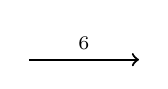
\begin{tikzpicture}[x=0.70cm,y=0.70cm]
\draw[->,thick] (0,0.5) -- (2.0,0.5);
\node at (1.0,0.8) {\scriptsize 6};
\end{tikzpicture}
\begin{tikzpicture}[x=0.70cm,y=0.70cm]
\node[anchor=east] at (-0.6,1.6) {E7};
\node[anchor=east] at (-0.6,1.2) {fret 9};
\draw (0.0,0.000) -- (0.0,1);
\draw (1.0,0.000) -- (1.0,1);
\draw (2.0,0.000) -- (2.0,1);
\draw (3.0,0.000) -- (3.0,1);
\draw (0.0,1.000) -- (3.0,1.000);
\node[anchor=east] at (-0.20,1.000) {\scriptsize 9};
\draw (0.0,0.667) -- (3.0,0.667);
\node[anchor=east] at (-0.20,0.667) {\scriptsize 10};
\draw (0.0,0.333) -- (3.0,0.333);
\node[anchor=east] at (-0.20,0.333) {\scriptsize 11};
\draw (0.0,0.000) -- (3.0,0.000);
\node[anchor=east] at (-0.20,0.000) {\scriptsize 12};
\node at (0.0,1.583) {\scriptsize 1};
\node at (1.0,1.583) {\scriptsize 3};
\node at (2.0,1.583) {\scriptsize 2};
\node at (3.0,1.583) {\scriptsize 4};
\fill[red] (0.0,1.000) circle (0.10);
\fill[black] (1.0,0.333) circle (0.10);
\fill[black] (2.0,0.667) circle (0.10);
\fill[black] (3.0,0.333) circle (0.10);
\node[anchor=west] at (0.0,-0.3) {\scriptsize grip: 1-5-b7-3};
\node[anchor=west] at (0.0,-0.6) {\scriptsize E3 B3 D5 A♭4};
\node[anchor=west] at (0.0,-0.9) {\scriptsize cost: 3};
\end{tikzpicture}
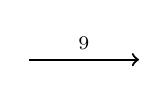
\begin{tikzpicture}[x=0.70cm,y=0.70cm]
\draw[->,thick] (0,0.5) -- (2.0,0.5);
\node at (1.0,0.8) {\scriptsize 9};
\end{tikzpicture}
\begin{tikzpicture}[x=0.70cm,y=0.70cm]
\node[anchor=east] at (-0.6,1.6) {A};
\node[anchor=east] at (-0.6,1.2) {fret 9};
\draw (0.0,0.000) -- (0.0,1);
\draw (1.0,0.000) -- (1.0,1);
\draw (2.0,0.000) -- (2.0,1);
\draw (3.0,0.000) -- (3.0,1);
\draw (0.0,1.000) -- (3.0,1.000);
\node[anchor=east] at (-0.20,1.000) {\scriptsize 9};
\draw (0.0,0.667) -- (3.0,0.667);
\node[anchor=east] at (-0.20,0.667) {\scriptsize 10};
\draw (0.0,0.333) -- (3.0,0.333);
\node[anchor=east] at (-0.20,0.333) {\scriptsize 11};
\draw (0.0,0.000) -- (3.0,0.000);
\node[anchor=east] at (-0.20,0.000) {\scriptsize 12};
\node at (0.0,1.583) {\scriptsize 1};
\node at (1.0,1.583) {\scriptsize 1};
\node at (2.0,1.583) {\scriptsize 1};
\node at (3.0,1.583) {\scriptsize 4};
\fill[black] (0.0,1.000) circle (0.10);
\fill[red] (1.0,1.000) circle (0.10);
\fill[black] (2.0,1.000) circle (0.10);
\fill[red] (3.0,0.000) circle (0.10);
\node[anchor=west] at (0.0,-0.3) {\scriptsize grip: 5-1-3-1};
\node[anchor=west] at (0.0,-0.6) {\scriptsize E3 A3 C♯5 A4};
\node[anchor=west] at (0.0,-0.9) {\scriptsize cost: 1};
\end{tikzpicture}
\end{minipage} & \begin{minipage}[t]{0.09\linewidth}\raggedleft\textit{total cost: 22}\end{minipage}\\
\end{tabular}
\bigskip
\subsection*{D (ii-V-I)}
\begin{tabular}{@{}p{0.89\linewidth}r@{}}
\begin{minipage}[t]{0.89\linewidth}\raggedright
\textit{Em A7 D}\\
\begin{tikzpicture}[x=0.70cm,y=0.70cm]
\node[anchor=east] at (-0.6,1.6) {Em};
\node[anchor=east] at (-0.6,1.2) {fret 10};
\draw (0.0,0.000) -- (0.0,1);
\draw (1.0,0.000) -- (1.0,1);
\draw (2.0,0.000) -- (2.0,1);
\draw (3.0,0.000) -- (3.0,1);
\draw (0.0,1.000) -- (3.0,1.000);
\node[anchor=east] at (-0.20,1.000) {\scriptsize 10};
\draw (0.0,0.667) -- (3.0,0.667);
\node[anchor=east] at (-0.20,0.667) {\scriptsize 11};
\draw (0.0,0.333) -- (3.0,0.333);
\node[anchor=east] at (-0.20,0.333) {\scriptsize 12};
\draw (0.0,0.000) -- (3.0,0.000);
\node[anchor=east] at (-0.20,0.000) {\scriptsize 13};
\node at (0.0,1.583) {\scriptsize 3};
\node at (1.0,1.583) {\scriptsize 2};
\node at (2.0,1.583) {\scriptsize 4};
\node at (3.0,1.583) {\scriptsize 1};
\fill[black] (0.0,0.333) circle (0.10);
\fill[black] (1.0,0.667) circle (0.10);
\fill[red] (2.0,0.333) circle (0.10);
\fill[black] (3.0,1.000) circle (0.10);
\node[anchor=west] at (0.0,-0.3) {\scriptsize grip: b3-5-1-b3};
\node[anchor=west] at (0.0,-0.6) {\scriptsize G3 B3 E5 G4};
\node[anchor=west] at (0.0,-0.9) {\scriptsize cost: 3};
\end{tikzpicture}
\begin{tikzpicture}[x=0.70cm,y=0.70cm]
\draw[->,thick] (0,0.5) -- (2.0,0.5);
\node at (1.0,0.8) {\scriptsize 5};
\end{tikzpicture}
\begin{tikzpicture}[x=0.70cm,y=0.70cm]
\node[anchor=east] at (-0.6,1.6) {A7};
\node[anchor=east] at (-0.6,1.2) {fret 12};
\draw (0.0,0.000) -- (0.0,1);
\draw (1.0,0.000) -- (1.0,1);
\draw (2.0,0.000) -- (2.0,1);
\draw (3.0,0.000) -- (3.0,1);
\draw (0.0,1.000) -- (3.0,1.000);
\node[anchor=east] at (-0.20,1.000) {\scriptsize 12};
\draw (0.0,0.667) -- (3.0,0.667);
\node[anchor=east] at (-0.20,0.667) {\scriptsize 13};
\draw (0.0,0.333) -- (3.0,0.333);
\node[anchor=east] at (-0.20,0.333) {\scriptsize 14};
\draw (0.0,0.000) -- (3.0,0.000);
\node[anchor=east] at (-0.20,0.000) {\scriptsize 15};
\node at (0.0,1.583) {\scriptsize 1};
\node at (1.0,1.583) {\scriptsize 2};
\node at (2.0,1.583) {\scriptsize 1};
\node at (3.0,1.583) {\scriptsize 1};
\fill[black] (0.0,1.000) circle (0.10);
\fill[black] (1.0,0.667) circle (0.10);
\fill[black] (2.0,1.000) circle (0.10);
\fill[red] (3.0,1.000) circle (0.10);
\node[anchor=west] at (0.0,-0.3) {\scriptsize grip: b7-3-5-1};
\node[anchor=west] at (0.0,-0.6) {\scriptsize G3 C♯4 E5 A4};
\node[anchor=west] at (0.0,-0.9) {\scriptsize cost: 0};
\end{tikzpicture}
\begin{tikzpicture}[x=0.70cm,y=0.70cm]
\draw[->,thick] (0,0.5) -- (2.0,0.5);
\node at (1.0,0.8) {\scriptsize 10};
\end{tikzpicture}
\begin{tikzpicture}[x=0.70cm,y=0.70cm]
\node[anchor=east] at (-0.6,1.6) {D};
\node[anchor=east] at (-0.6,1.2) {fret 12};
\draw (0.0,0.000) -- (0.0,1);
\draw (1.0,0.000) -- (1.0,1);
\draw (2.0,0.000) -- (2.0,1);
\draw (3.0,0.000) -- (3.0,1);
\draw (0.0,1.000) -- (3.0,1.000);
\node[anchor=east] at (-0.20,1.000) {\scriptsize 12};
\draw (0.0,0.667) -- (3.0,0.667);
\node[anchor=east] at (-0.20,0.667) {\scriptsize 13};
\draw (0.0,0.333) -- (3.0,0.333);
\node[anchor=east] at (-0.20,0.333) {\scriptsize 14};
\draw (0.0,0.000) -- (3.0,0.000);
\node[anchor=east] at (-0.20,0.000) {\scriptsize 15};
\node at (0.0,1.583) {\scriptsize 2};
\node at (1.0,1.583) {\scriptsize 3};
\node at (2.0,1.583) {\scriptsize 4};
\node at (3.0,1.583) {\scriptsize 1};
\fill[black] (0.0,0.333) circle (0.10);
\fill[red] (1.0,0.333) circle (0.10);
\fill[black] (2.0,0.333) circle (0.10);
\fill[black] (3.0,1.000) circle (0.10);
\node[anchor=west] at (0.0,-0.3) {\scriptsize grip: 5-1-3-5};
\node[anchor=west] at (0.0,-0.6) {\scriptsize A3 D4 F♯5 A4};
\node[anchor=west] at (0.0,-0.9) {\scriptsize cost: 4};
\end{tikzpicture}
\end{minipage} & \begin{minipage}[t]{0.09\linewidth}\raggedleft\textit{total cost: 22}\end{minipage}\\
\end{tabular}
\bigskip
\subsection*{G (ii-V-I)}
\begin{tabular}{@{}p{0.89\linewidth}r@{}}
\begin{minipage}[t]{0.89\linewidth}\raggedright
\textit{Am D7 G}\\
\begin{tikzpicture}[x=0.70cm,y=0.70cm]
\node[anchor=east] at (-0.6,1.6) {Am};
\node[anchor=east] at (-0.6,1.2) {fret 2};
\draw (0.0,0.000) -- (0.0,1);
\draw (1.0,0.000) -- (1.0,1);
\draw (2.0,0.000) -- (2.0,1);
\draw (3.0,0.000) -- (3.0,1);
\draw (0.0,1.000) -- (3.0,1.000);
\node[anchor=east] at (-0.20,1.000) {\scriptsize 2};
\draw (0.0,0.667) -- (3.0,0.667);
\node[anchor=east] at (-0.20,0.667) {\scriptsize 3};
\draw (0.0,0.333) -- (3.0,0.333);
\node[anchor=east] at (-0.20,0.333) {\scriptsize 4};
\draw (0.0,0.000) -- (3.0,0.000);
\node[anchor=east] at (-0.20,0.000) {\scriptsize 5};
\draw[line width=0.8pt] (0,1.333) -- (3.0,1.333);
\node at (0.0,1.583) {\scriptsize 3};
\fill[red] (0.0,1.000) circle (0.10);
\draw (1.0,1.333) circle (0.08);
\draw (2.0,1.333) circle (0.08);
\draw[red] (3.0,1.333) circle (0.08);
\node[anchor=west] at (0.0,-0.3) {\scriptsize grip: 1-b3-5-1};
\node[anchor=west] at (0.0,-0.6) {\scriptsize A2 C3 E4 A3};
\node[anchor=west] at (0.0,-0.9) {\scriptsize cost: 2};
\end{tikzpicture}
\begin{tikzpicture}[x=0.70cm,y=0.70cm]
\draw[->,thick] (0,0.5) -- (2.0,0.5);
\node at (1.0,0.8) {\scriptsize 2};
\end{tikzpicture}
\begin{tikzpicture}[x=0.70cm,y=0.70cm]
\node[anchor=east] at (-0.6,1.6) {D7};
\node[anchor=east] at (-0.6,1.2) {fret 2};
\draw (0.0,0.000) -- (0.0,1);
\draw (1.0,0.000) -- (1.0,1);
\draw (2.0,0.000) -- (2.0,1);
\draw (3.0,0.000) -- (3.0,1);
\draw (0.0,1.000) -- (3.0,1.000);
\node[anchor=east] at (-0.20,1.000) {\scriptsize 2};
\draw (0.0,0.667) -- (3.0,0.667);
\node[anchor=east] at (-0.20,0.667) {\scriptsize 3};
\draw (0.0,0.333) -- (3.0,0.333);
\node[anchor=east] at (-0.20,0.333) {\scriptsize 4};
\draw (0.0,0.000) -- (3.0,0.000);
\node[anchor=east] at (-0.20,0.000) {\scriptsize 5};
\node at (0.0,1.583) {\scriptsize 1};
\node at (1.0,1.583) {\scriptsize 1};
\node at (2.0,1.583) {\scriptsize 1};
\node at (3.0,1.583) {\scriptsize 2};
\fill[black] (0.0,1.000) circle (0.10);
\fill[red] (1.0,1.000) circle (0.10);
\fill[black] (2.0,1.000) circle (0.10);
\fill[black] (3.0,0.667) circle (0.10);
\node[anchor=west] at (0.0,-0.3) {\scriptsize grip: 5-1-3-b7};
\node[anchor=west] at (0.0,-0.6) {\scriptsize A2 D3 F♯4 C4};
\node[anchor=west] at (0.0,-0.9) {\scriptsize cost: 0};
\end{tikzpicture}
\begin{tikzpicture}[x=0.70cm,y=0.70cm]
\draw[->,thick] (0,0.5) -- (2.0,0.5);
\node at (1.0,0.8) {\scriptsize 6};
\end{tikzpicture}
\begin{tikzpicture}[x=0.70cm,y=0.70cm]
\node[anchor=east] at (-0.6,1.6) {G};
\node[anchor=east] at (-0.6,1.2) {fret 2};
\draw (0.0,0.000) -- (0.0,1);
\draw (1.0,0.000) -- (1.0,1);
\draw (2.0,0.000) -- (2.0,1);
\draw (3.0,0.000) -- (3.0,1);
\draw (0.0,1.000) -- (3.0,1.000);
\node[anchor=east] at (-0.20,1.000) {\scriptsize 2};
\draw (0.0,0.667) -- (3.0,0.667);
\node[anchor=east] at (-0.20,0.667) {\scriptsize 3};
\draw (0.0,0.333) -- (3.0,0.333);
\node[anchor=east] at (-0.20,0.333) {\scriptsize 4};
\draw (0.0,0.000) -- (3.0,0.000);
\node[anchor=east] at (-0.20,0.000) {\scriptsize 5};
\draw[line width=0.8pt] (0,1.333) -- (3.0,1.333);
\node at (1.0,1.583) {\scriptsize 1};
\node at (2.0,1.583) {\scriptsize 2};
\node at (3.0,1.583) {\scriptsize 1};
\draw[red] (0.0,1.333) circle (0.08);
\fill[black] (1.0,1.000) circle (0.10);
\fill[red] (2.0,0.667) circle (0.10);
\fill[black] (3.0,1.000) circle (0.10);
\node[anchor=west] at (0.0,-0.3) {\scriptsize grip: 1-5-1-3};
\node[anchor=west] at (0.0,-0.6) {\scriptsize G2 D3 G4 B3};
\node[anchor=west] at (0.0,-0.9) {\scriptsize cost: 2};
\end{tikzpicture}
\end{minipage} & \begin{minipage}[t]{0.09\linewidth}\raggedleft\textit{total cost: 12}\end{minipage}\\
\end{tabular}
\bigskip
\section*{FUTON5 ii-V-I cheat sheet (open drone variants)}
\subsection*{C (ii-V-I)}
\begin{tabular}{@{}p{0.89\linewidth}r@{}}
\begin{minipage}[t]{0.89\linewidth}\raggedright
\textit{Dm7 G7add11 C}\\
\begin{tikzpicture}[x=0.55cm,y=0.55cm]
\node[anchor=east] at (-0.6,1.6) {Dm7};
\node[anchor=east] at (-0.6,1.2) {fret 12};
\draw (0.0,1.333) -- (0.0,1);
\draw (1.0,0.000) -- (1.0,1);
\draw (2.0,0.000) -- (2.0,1);
\draw (3.0,0.000) -- (3.0,1);
\draw (4.0,0.000) -- (4.0,1);
\draw (1.0,1.000) -- (4.0,1.000);
\node[anchor=east] at (-0.20,1.000) {\scriptsize 12};
\draw (1.0,0.667) -- (4.0,0.667);
\node[anchor=east] at (-0.20,0.667) {\scriptsize 13};
\draw (1.0,0.333) -- (4.0,0.333);
\node[anchor=east] at (-0.20,0.333) {\scriptsize 14};
\draw (1.0,0.000) -- (4.0,0.000);
\node[anchor=east] at (-0.20,0.000) {\scriptsize 15};
\draw[line width=0.8pt] (0,1.333) -- (4.0,1.333);
\node at (1.0,1.583) {\scriptsize 3};
\node at (2.0,1.583) {\scriptsize 4};
\node at (3.0,1.583) {\scriptsize 2};
\node at (4.0,1.583) {\scriptsize 1};
\draw (0.0,1.333) circle (0.08);
\fill[black] (1.0,0.333) circle (0.10);
\fill[red] (2.0,0.333) circle (0.10);
\fill[black] (3.0,0.667) circle (0.10);
\fill[black] (4.0,1.000) circle (0.10);
\node[anchor=west] at (0.0,-0.3) {\scriptsize grip: 5-1-b3-5};
\node[anchor=west] at (0.0,-0.6) {\scriptsize C4 A3 D4 F5 A4};
\node[anchor=west] at (0.0,-0.9) {\scriptsize cost: 3};
\end{tikzpicture}
\begin{tikzpicture}[x=0.55cm,y=0.55cm]
\draw[->,thick] (0,0.5) -- (2.0,0.5);
\node at (1.0,0.8) {\scriptsize 6};
\end{tikzpicture}
\begin{tikzpicture}[x=0.55cm,y=0.55cm]
\node[anchor=east] at (-0.6,1.6) {G7add11};
\node[anchor=east] at (-0.6,1.2) {fret 12};
\draw (0.0,1.333) -- (0.0,1);
\draw (1.0,0.000) -- (1.0,1);
\draw (2.0,0.000) -- (2.0,1);
\draw (3.0,0.000) -- (3.0,1);
\draw (4.0,0.000) -- (4.0,1);
\draw (1.0,1.000) -- (4.0,1.000);
\node[anchor=east] at (-0.20,1.000) {\scriptsize 12};
\draw (1.0,0.667) -- (4.0,0.667);
\node[anchor=east] at (-0.20,0.667) {\scriptsize 13};
\draw (1.0,0.333) -- (4.0,0.333);
\node[anchor=east] at (-0.20,0.333) {\scriptsize 14};
\draw (1.0,0.000) -- (4.0,0.000);
\node[anchor=east] at (-0.20,0.000) {\scriptsize 15};
\draw[line width=0.8pt] (0,1.333) -- (4.0,1.333);
\node at (1.0,1.583) {\scriptsize 1};
\node at (2.0,1.583) {\scriptsize 3};
\node at (3.0,1.583) {\scriptsize 2};
\node at (4.0,1.583) {\scriptsize 4};
\draw (0.0,1.333) circle (0.08);
\fill[red] (1.0,1.000) circle (0.10);
\fill[black] (2.0,0.333) circle (0.10);
\fill[black] (3.0,0.667) circle (0.10);
\fill[black] (4.0,0.333) circle (0.10);
\node[anchor=west] at (0.0,-0.3) {\scriptsize grip: 1-5-b7-3};
\node[anchor=west] at (0.0,-0.6) {\scriptsize C4 G3 D4 F5 B4};
\node[anchor=west] at (0.0,-0.9) {\scriptsize cost: 3};
\end{tikzpicture}
\begin{tikzpicture}[x=0.55cm,y=0.55cm]
\draw[->,thick] (0,0.5) -- (2.0,0.5);
\node at (1.0,0.8) {\scriptsize 9};
\end{tikzpicture}
\begin{tikzpicture}[x=0.55cm,y=0.55cm]
\node[anchor=east] at (-0.6,1.6) {C};
\node[anchor=east] at (-0.6,1.2) {fret 12};
\draw (0.0,1.333) -- (0.0,1);
\draw (1.0,0.000) -- (1.0,1);
\draw (2.0,0.000) -- (2.0,1);
\draw (3.0,0.000) -- (3.0,1);
\draw (4.0,0.000) -- (4.0,1);
\draw (1.0,1.000) -- (4.0,1.000);
\node[anchor=east] at (-0.20,1.000) {\scriptsize 12};
\draw (1.0,0.667) -- (4.0,0.667);
\node[anchor=east] at (-0.20,0.667) {\scriptsize 13};
\draw (1.0,0.333) -- (4.0,0.333);
\node[anchor=east] at (-0.20,0.333) {\scriptsize 14};
\draw (1.0,0.000) -- (4.0,0.000);
\node[anchor=east] at (-0.20,0.000) {\scriptsize 15};
\draw[line width=0.8pt] (0,1.333) -- (4.0,1.333);
\node at (1.0,1.583) {\scriptsize 1};
\node at (2.0,1.583) {\scriptsize 1};
\node at (3.0,1.583) {\scriptsize 1};
\node at (4.0,1.583) {\scriptsize 4};
\draw[red] (0.0,1.333) circle (0.08);
\fill[black] (1.0,1.000) circle (0.10);
\fill[red] (2.0,1.000) circle (0.10);
\fill[black] (3.0,1.000) circle (0.10);
\fill[red] (4.0,0.000) circle (0.10);
\node[anchor=west] at (0.0,-0.3) {\scriptsize grip: 5-1-3-1};
\node[anchor=west] at (0.0,-0.6) {\scriptsize C4 G3 C4 E5 C5};
\node[anchor=west] at (0.0,-0.9) {\scriptsize cost: 1};
\end{tikzpicture}
\end{minipage} & \begin{minipage}[t]{0.09\linewidth}\raggedleft\textit{total cost: 22}\end{minipage}\\
\end{tabular}
\bigskip
\subsection*{F (ii-V-I)}
\begin{tabular}{@{}p{0.89\linewidth}r@{}}
\begin{minipage}[t]{0.89\linewidth}\raggedright
\textit{Gmadd11 C7 F}\\
\begin{tikzpicture}[x=0.55cm,y=0.55cm]
\node[anchor=east] at (-0.6,1.6) {Gmadd11};
\node[anchor=east] at (-0.6,1.2) {fret 10};
\draw (0.0,1.333) -- (0.0,1);
\draw (1.0,0.000) -- (1.0,1);
\draw (2.0,0.000) -- (2.0,1);
\draw (3.0,0.000) -- (3.0,1);
\draw (4.0,0.000) -- (4.0,1);
\draw (1.0,1.000) -- (4.0,1.000);
\node[anchor=east] at (-0.20,1.000) {\scriptsize 10};
\draw (1.0,0.667) -- (4.0,0.667);
\node[anchor=east] at (-0.20,0.667) {\scriptsize 11};
\draw (1.0,0.333) -- (4.0,0.333);
\node[anchor=east] at (-0.20,0.333) {\scriptsize 12};
\draw (1.0,0.000) -- (4.0,0.000);
\node[anchor=east] at (-0.20,0.000) {\scriptsize 13};
\draw[line width=0.8pt] (0,1.333) -- (4.0,1.333);
\node at (1.0,1.583) {\scriptsize 3};
\node at (2.0,1.583) {\scriptsize 1};
\node at (3.0,1.583) {\scriptsize 1};
\node at (4.0,1.583) {\scriptsize 1};
\draw (0.0,1.333) circle (0.08);
\fill[red] (1.0,0.333) circle (0.10);
\fill[black] (2.0,1.000) circle (0.10);
\fill[black] (3.0,1.000) circle (0.10);
\fill[red] (4.0,1.000) circle (0.10);
\node[anchor=west] at (0.0,-0.3) {\scriptsize grip: 1-b3-5-1};
\node[anchor=west] at (0.0,-0.6) {\scriptsize C4 G3 B♭3 D5 G4};
\node[anchor=west] at (0.0,-0.9) {\scriptsize cost: 0};
\end{tikzpicture}
\begin{tikzpicture}[x=0.55cm,y=0.55cm]
\draw[->,thick] (0,0.5) -- (2.0,0.5);
\node at (1.0,0.8) {\scriptsize 6};
\end{tikzpicture}
\begin{tikzpicture}[x=0.55cm,y=0.55cm]
\node[anchor=east] at (-0.6,1.6) {C7};
\node[anchor=east] at (-0.6,1.2) {fret 8};
\draw (0.0,1.333) -- (0.0,1);
\draw (1.0,0.000) -- (1.0,1);
\draw (2.0,0.000) -- (2.0,1);
\draw (3.0,0.000) -- (3.0,1);
\draw (4.0,0.000) -- (4.0,1);
\draw (1.0,1.000) -- (4.0,1.000);
\node[anchor=east] at (-0.20,1.000) {\scriptsize 8};
\draw (1.0,0.667) -- (4.0,0.667);
\node[anchor=east] at (-0.20,0.667) {\scriptsize 9};
\draw (1.0,0.333) -- (4.0,0.333);
\node[anchor=east] at (-0.20,0.333) {\scriptsize 10};
\draw (1.0,0.000) -- (4.0,0.000);
\node[anchor=east] at (-0.20,0.000) {\scriptsize 11};
\draw[line width=0.8pt] (0,1.333) -- (4.0,1.333);
\node at (1.0,1.583) {\scriptsize 2};
\node at (2.0,1.583) {\scriptsize 3};
\node at (3.0,1.583) {\scriptsize 1};
\node at (4.0,1.583) {\scriptsize 4};
\draw[red] (0.0,1.333) circle (0.08);
\fill[black] (1.0,0.667) circle (0.10);
\fill[black] (2.0,0.333) circle (0.10);
\fill[red] (3.0,1.000) circle (0.10);
\fill[black] (4.0,0.333) circle (0.10);
\node[anchor=west] at (0.0,-0.3) {\scriptsize grip: 3-b7-1-5};
\node[anchor=west] at (0.0,-0.6) {\scriptsize C4 E3 B♭3 C5 G4};
\node[anchor=west] at (0.0,-0.9) {\scriptsize cost: 3};
\end{tikzpicture}
\begin{tikzpicture}[x=0.55cm,y=0.55cm]
\draw[->,thick] (0,0.5) -- (2.0,0.5);
\node at (1.0,0.8) {\scriptsize 9};
\end{tikzpicture}
\begin{tikzpicture}[x=0.55cm,y=0.55cm]
\node[anchor=east] at (-0.6,1.6) {F};
\node[anchor=east] at (-0.6,1.2) {fret 8};
\draw (0.0,1.333) -- (0.0,1);
\draw (1.0,0.000) -- (1.0,1);
\draw (2.0,0.000) -- (2.0,1);
\draw (3.0,0.000) -- (3.0,1);
\draw (4.0,0.000) -- (4.0,1);
\draw (1.0,1.000) -- (4.0,1.000);
\node[anchor=east] at (-0.20,1.000) {\scriptsize 8};
\draw (1.0,0.667) -- (4.0,0.667);
\node[anchor=east] at (-0.20,0.667) {\scriptsize 9};
\draw (1.0,0.333) -- (4.0,0.333);
\node[anchor=east] at (-0.20,0.333) {\scriptsize 10};
\draw (1.0,0.000) -- (4.0,0.000);
\node[anchor=east] at (-0.20,0.000) {\scriptsize 11};
\draw[line width=0.8pt] (0,1.333) -- (4.0,1.333);
\node at (1.0,1.583) {\scriptsize 3};
\node at (2.0,1.583) {\scriptsize 2};
\node at (3.0,1.583) {\scriptsize 1};
\node at (4.0,1.583) {\scriptsize 1};
\draw (0.0,1.333) circle (0.08);
\fill[red] (1.0,0.333) circle (0.10);
\fill[black] (2.0,0.667) circle (0.10);
\fill[black] (3.0,1.000) circle (0.10);
\fill[red] (4.0,1.000) circle (0.10);
\node[anchor=west] at (0.0,-0.3) {\scriptsize grip: 1-3-5-1};
\node[anchor=west] at (0.0,-0.6) {\scriptsize C4 F3 A3 C5 F4};
\node[anchor=west] at (0.0,-0.9) {\scriptsize cost: 1};
\end{tikzpicture}
\end{minipage} & \begin{minipage}[t]{0.09\linewidth}\raggedleft\textit{total cost: 19}\end{minipage}\\
\end{tabular}
\bigskip
\subsection*{Bb (ii-V-I)}
\begin{tabular}{@{}p{0.89\linewidth}r@{}}
\begin{minipage}[t]{0.89\linewidth}\raggedright
\textit{Cm F7 B♭add9}\\
\begin{tikzpicture}[x=0.55cm,y=0.55cm]
\node[anchor=east] at (-0.6,1.6) {Cm};
\node[anchor=east] at (-0.6,1.2) {fret 10};
\draw (0.0,1.333) -- (0.0,1);
\draw (1.0,0.000) -- (1.0,1);
\draw (2.0,0.000) -- (2.0,1);
\draw (3.0,0.000) -- (3.0,1);
\draw (4.0,0.000) -- (4.0,1);
\draw (1.0,1.000) -- (4.0,1.000);
\node[anchor=east] at (-0.20,1.000) {\scriptsize 10};
\draw (1.0,0.667) -- (4.0,0.667);
\node[anchor=east] at (-0.20,0.667) {\scriptsize 11};
\draw (1.0,0.333) -- (4.0,0.333);
\node[anchor=east] at (-0.20,0.333) {\scriptsize 12};
\draw (1.0,0.000) -- (4.0,0.000);
\node[anchor=east] at (-0.20,0.000) {\scriptsize 13};
\draw[line width=0.8pt] (0,1.333) -- (4.0,1.333);
\node at (1.0,1.583) {\scriptsize 3};
\node at (2.0,1.583) {\scriptsize 4};
\node at (3.0,1.583) {\scriptsize 2};
\node at (4.0,1.583) {\scriptsize 1};
\draw[red] (0.0,1.333) circle (0.08);
\fill[black] (1.0,0.333) circle (0.10);
\fill[red] (2.0,0.333) circle (0.10);
\fill[black] (3.0,0.667) circle (0.10);
\fill[black] (4.0,1.000) circle (0.10);
\node[anchor=west] at (0.0,-0.3) {\scriptsize grip: 5-1-b3-5};
\node[anchor=west] at (0.0,-0.6) {\scriptsize C4 G3 C4 E♭5 G4};
\node[anchor=west] at (0.0,-0.9) {\scriptsize cost: 3};
\end{tikzpicture}
\begin{tikzpicture}[x=0.55cm,y=0.55cm]
\draw[->,thick] (0,0.5) -- (2.0,0.5);
\node at (1.0,0.8) {\scriptsize 6};
\end{tikzpicture}
\begin{tikzpicture}[x=0.55cm,y=0.55cm]
\node[anchor=east] at (-0.6,1.6) {F7};
\node[anchor=east] at (-0.6,1.2) {fret 10};
\draw (0.0,1.333) -- (0.0,1);
\draw (1.0,0.000) -- (1.0,1);
\draw (2.0,0.000) -- (2.0,1);
\draw (3.0,0.000) -- (3.0,1);
\draw (4.0,0.000) -- (4.0,1);
\draw (1.0,1.000) -- (4.0,1.000);
\node[anchor=east] at (-0.20,1.000) {\scriptsize 10};
\draw (1.0,0.667) -- (4.0,0.667);
\node[anchor=east] at (-0.20,0.667) {\scriptsize 11};
\draw (1.0,0.333) -- (4.0,0.333);
\node[anchor=east] at (-0.20,0.333) {\scriptsize 12};
\draw (1.0,0.000) -- (4.0,0.000);
\node[anchor=east] at (-0.20,0.000) {\scriptsize 13};
\draw[line width=0.8pt] (0,1.333) -- (4.0,1.333);
\node at (1.0,1.583) {\scriptsize 1};
\node at (2.0,1.583) {\scriptsize 3};
\node at (3.0,1.583) {\scriptsize 2};
\node at (4.0,1.583) {\scriptsize 4};
\draw (0.0,1.333) circle (0.08);
\fill[red] (1.0,1.000) circle (0.10);
\fill[black] (2.0,0.333) circle (0.10);
\fill[black] (3.0,0.667) circle (0.10);
\fill[black] (4.0,0.333) circle (0.10);
\node[anchor=west] at (0.0,-0.3) {\scriptsize grip: 1-5-b7-3};
\node[anchor=west] at (0.0,-0.6) {\scriptsize C4 F3 C4 E♭5 A4};
\node[anchor=west] at (0.0,-0.9) {\scriptsize cost: 3};
\end{tikzpicture}
\begin{tikzpicture}[x=0.55cm,y=0.55cm]
\draw[->,thick] (0,0.5) -- (2.0,0.5);
\node at (1.0,0.8) {\scriptsize 9};
\end{tikzpicture}
\begin{tikzpicture}[x=0.55cm,y=0.55cm]
\node[anchor=east] at (-0.6,1.6) {B♭add9};
\node[anchor=east] at (-0.6,1.2) {fret 10};
\draw (0.0,1.333) -- (0.0,1);
\draw (1.0,0.000) -- (1.0,1);
\draw (2.0,0.000) -- (2.0,1);
\draw (3.0,0.000) -- (3.0,1);
\draw (4.0,0.000) -- (4.0,1);
\draw (1.0,1.000) -- (4.0,1.000);
\node[anchor=east] at (-0.20,1.000) {\scriptsize 10};
\draw (1.0,0.667) -- (4.0,0.667);
\node[anchor=east] at (-0.20,0.667) {\scriptsize 11};
\draw (1.0,0.333) -- (4.0,0.333);
\node[anchor=east] at (-0.20,0.333) {\scriptsize 12};
\draw (1.0,0.000) -- (4.0,0.000);
\node[anchor=east] at (-0.20,0.000) {\scriptsize 13};
\draw[line width=0.8pt] (0,1.333) -- (4.0,1.333);
\node at (1.0,1.583) {\scriptsize 1};
\node at (2.0,1.583) {\scriptsize 1};
\node at (3.0,1.583) {\scriptsize 1};
\node at (4.0,1.583) {\scriptsize 4};
\draw (0.0,1.333) circle (0.08);
\fill[black] (1.0,1.000) circle (0.10);
\fill[red] (2.0,1.000) circle (0.10);
\fill[black] (3.0,1.000) circle (0.10);
\fill[red] (4.0,0.000) circle (0.10);
\node[anchor=west] at (0.0,-0.3) {\scriptsize grip: 5-1-3-1};
\node[anchor=west] at (0.0,-0.6) {\scriptsize C4 F3 B♭3 D5 B♭4};
\node[anchor=west] at (0.0,-0.9) {\scriptsize cost: 1};
\end{tikzpicture}
\end{minipage} & \begin{minipage}[t]{0.09\linewidth}\raggedleft\textit{total cost: 22}\end{minipage}\\
\end{tabular}
\bigskip
\subsection*{Eb (ii-V-I)}
\begin{tabular}{@{}p{0.89\linewidth}r@{}}
\begin{minipage}[t]{0.89\linewidth}\raggedright
\textit{Fm B♭7add9 E♭6}\\
\begin{tikzpicture}[x=0.55cm,y=0.55cm]
\node[anchor=east] at (-0.6,1.6) {Fm};
\node[anchor=east] at (-0.6,1.2) {fret 8};
\draw (0.0,1.333) -- (0.0,1);
\draw (1.0,0.000) -- (1.0,1);
\draw (2.0,0.000) -- (2.0,1);
\draw (3.0,0.000) -- (3.0,1);
\draw (4.0,0.000) -- (4.0,1);
\draw (1.0,1.000) -- (4.0,1.000);
\node[anchor=east] at (-0.20,1.000) {\scriptsize 8};
\draw (1.0,0.667) -- (4.0,0.667);
\node[anchor=east] at (-0.20,0.667) {\scriptsize 9};
\draw (1.0,0.333) -- (4.0,0.333);
\node[anchor=east] at (-0.20,0.333) {\scriptsize 10};
\draw (1.0,0.000) -- (4.0,0.000);
\node[anchor=east] at (-0.20,0.000) {\scriptsize 11};
\draw[line width=0.8pt] (0,1.333) -- (4.0,1.333);
\node at (1.0,1.583) {\scriptsize 3};
\node at (2.0,1.583) {\scriptsize 1};
\node at (3.0,1.583) {\scriptsize 1};
\node at (4.0,1.583) {\scriptsize 1};
\draw (0.0,1.333) circle (0.08);
\fill[red] (1.0,0.333) circle (0.10);
\fill[black] (2.0,1.000) circle (0.10);
\fill[black] (3.0,1.000) circle (0.10);
\fill[red] (4.0,1.000) circle (0.10);
\node[anchor=west] at (0.0,-0.3) {\scriptsize grip: 1-b3-5-1};
\node[anchor=west] at (0.0,-0.6) {\scriptsize C4 F3 A♭3 C5 F4};
\node[anchor=west] at (0.0,-0.9) {\scriptsize cost: 0};
\end{tikzpicture}
\begin{tikzpicture}[x=0.55cm,y=0.55cm]
\draw[->,thick] (0,0.5) -- (2.0,0.5);
\node at (1.0,0.8) {\scriptsize 6};
\end{tikzpicture}
\begin{tikzpicture}[x=0.55cm,y=0.55cm]
\node[anchor=east] at (-0.6,1.6) {B♭7add9};
\node[anchor=east] at (-0.6,1.2) {fret 6};
\draw (0.0,1.333) -- (0.0,1);
\draw (1.0,0.000) -- (1.0,1);
\draw (2.0,0.000) -- (2.0,1);
\draw (3.0,0.000) -- (3.0,1);
\draw (4.0,0.000) -- (4.0,1);
\draw (1.0,1.000) -- (4.0,1.000);
\node[anchor=east] at (-0.20,1.000) {\scriptsize 6};
\draw (1.0,0.667) -- (4.0,0.667);
\node[anchor=east] at (-0.20,0.667) {\scriptsize 7};
\draw (1.0,0.333) -- (4.0,0.333);
\node[anchor=east] at (-0.20,0.333) {\scriptsize 8};
\draw (1.0,0.000) -- (4.0,0.000);
\node[anchor=east] at (-0.20,0.000) {\scriptsize 9};
\draw[line width=0.8pt] (0,1.333) -- (4.0,1.333);
\node at (1.0,1.583) {\scriptsize 2};
\node at (2.0,1.583) {\scriptsize 3};
\node at (3.0,1.583) {\scriptsize 1};
\node at (4.0,1.583) {\scriptsize 4};
\draw (0.0,1.333) circle (0.08);
\fill[black] (1.0,0.667) circle (0.10);
\fill[black] (2.0,0.333) circle (0.10);
\fill[red] (3.0,1.000) circle (0.10);
\fill[black] (4.0,0.333) circle (0.10);
\node[anchor=west] at (0.0,-0.3) {\scriptsize grip: 3-b7-1-5};
\node[anchor=west] at (0.0,-0.6) {\scriptsize C4 D3 A♭3 B♭4 F4};
\node[anchor=west] at (0.0,-0.9) {\scriptsize cost: 3};
\end{tikzpicture}
\begin{tikzpicture}[x=0.55cm,y=0.55cm]
\draw[->,thick] (0,0.5) -- (2.0,0.5);
\node at (1.0,0.8) {\scriptsize 9};
\end{tikzpicture}
\begin{tikzpicture}[x=0.55cm,y=0.55cm]
\node[anchor=east] at (-0.6,1.6) {E♭6};
\node[anchor=east] at (-0.6,1.2) {fret 6};
\draw (0.0,1.333) -- (0.0,1);
\draw (1.0,0.000) -- (1.0,1);
\draw (2.0,0.000) -- (2.0,1);
\draw (3.0,0.000) -- (3.0,1);
\draw (4.0,0.000) -- (4.0,1);
\draw (1.0,1.000) -- (4.0,1.000);
\node[anchor=east] at (-0.20,1.000) {\scriptsize 6};
\draw (1.0,0.667) -- (4.0,0.667);
\node[anchor=east] at (-0.20,0.667) {\scriptsize 7};
\draw (1.0,0.333) -- (4.0,0.333);
\node[anchor=east] at (-0.20,0.333) {\scriptsize 8};
\draw (1.0,0.000) -- (4.0,0.000);
\node[anchor=east] at (-0.20,0.000) {\scriptsize 9};
\draw[line width=0.8pt] (0,1.333) -- (4.0,1.333);
\node at (1.0,1.583) {\scriptsize 3};
\node at (2.0,1.583) {\scriptsize 2};
\node at (3.0,1.583) {\scriptsize 1};
\node at (4.0,1.583) {\scriptsize 1};
\draw (0.0,1.333) circle (0.08);
\fill[red] (1.0,0.333) circle (0.10);
\fill[black] (2.0,0.667) circle (0.10);
\fill[black] (3.0,1.000) circle (0.10);
\fill[red] (4.0,1.000) circle (0.10);
\node[anchor=west] at (0.0,-0.3) {\scriptsize grip: 1-3-5-1};
\node[anchor=west] at (0.0,-0.6) {\scriptsize C4 E♭3 G3 B♭4 E♭4};
\node[anchor=west] at (0.0,-0.9) {\scriptsize cost: 1};
\end{tikzpicture}
\end{minipage} & \begin{minipage}[t]{0.09\linewidth}\raggedleft\textit{total cost: 19}\end{minipage}\\
\end{tabular}
\bigskip
\subsection*{Ab (ii-V-I)}
\begin{tabular}{@{}p{0.89\linewidth}r@{}}
\begin{minipage}[t]{0.89\linewidth}\raggedright
\textit{B♭madd9 E♭76 A♭}\\
\begin{tikzpicture}[x=0.55cm,y=0.55cm]
\node[anchor=east] at (-0.6,1.6) {B♭madd9};
\node[anchor=east] at (-0.6,1.2) {fret 8};
\draw (0.0,1.333) -- (0.0,1);
\draw (1.0,0.000) -- (1.0,1);
\draw (2.0,0.000) -- (2.0,1);
\draw (3.0,0.000) -- (3.0,1);
\draw (4.0,0.000) -- (4.0,1);
\draw (1.0,1.000) -- (4.0,1.000);
\node[anchor=east] at (-0.20,1.000) {\scriptsize 8};
\draw (1.0,0.667) -- (4.0,0.667);
\node[anchor=east] at (-0.20,0.667) {\scriptsize 9};
\draw (1.0,0.333) -- (4.0,0.333);
\node[anchor=east] at (-0.20,0.333) {\scriptsize 10};
\draw (1.0,0.000) -- (4.0,0.000);
\node[anchor=east] at (-0.20,0.000) {\scriptsize 11};
\draw[line width=0.8pt] (0,1.333) -- (4.0,1.333);
\node at (1.0,1.583) {\scriptsize 3};
\node at (2.0,1.583) {\scriptsize 4};
\node at (3.0,1.583) {\scriptsize 2};
\node at (4.0,1.583) {\scriptsize 1};
\draw (0.0,1.333) circle (0.08);
\fill[black] (1.0,0.333) circle (0.10);
\fill[red] (2.0,0.333) circle (0.10);
\fill[black] (3.0,0.667) circle (0.10);
\fill[black] (4.0,1.000) circle (0.10);
\node[anchor=west] at (0.0,-0.3) {\scriptsize grip: 5-1-b3-5};
\node[anchor=west] at (0.0,-0.6) {\scriptsize C4 F3 B♭3 C♯5 F4};
\node[anchor=west] at (0.0,-0.9) {\scriptsize cost: 3};
\end{tikzpicture}
\begin{tikzpicture}[x=0.55cm,y=0.55cm]
\draw[->,thick] (0,0.5) -- (2.0,0.5);
\node at (1.0,0.8) {\scriptsize 6};
\end{tikzpicture}
\begin{tikzpicture}[x=0.55cm,y=0.55cm]
\node[anchor=east] at (-0.6,1.6) {E♭76};
\node[anchor=east] at (-0.6,1.2) {fret 8};
\draw (0.0,1.333) -- (0.0,1);
\draw (1.0,0.000) -- (1.0,1);
\draw (2.0,0.000) -- (2.0,1);
\draw (3.0,0.000) -- (3.0,1);
\draw (4.0,0.000) -- (4.0,1);
\draw (1.0,1.000) -- (4.0,1.000);
\node[anchor=east] at (-0.20,1.000) {\scriptsize 8};
\draw (1.0,0.667) -- (4.0,0.667);
\node[anchor=east] at (-0.20,0.667) {\scriptsize 9};
\draw (1.0,0.333) -- (4.0,0.333);
\node[anchor=east] at (-0.20,0.333) {\scriptsize 10};
\draw (1.0,0.000) -- (4.0,0.000);
\node[anchor=east] at (-0.20,0.000) {\scriptsize 11};
\draw[line width=0.8pt] (0,1.333) -- (4.0,1.333);
\node at (1.0,1.583) {\scriptsize 1};
\node at (2.0,1.583) {\scriptsize 3};
\node at (3.0,1.583) {\scriptsize 2};
\node at (4.0,1.583) {\scriptsize 4};
\draw (0.0,1.333) circle (0.08);
\fill[red] (1.0,1.000) circle (0.10);
\fill[black] (2.0,0.333) circle (0.10);
\fill[black] (3.0,0.667) circle (0.10);
\fill[black] (4.0,0.333) circle (0.10);
\node[anchor=west] at (0.0,-0.3) {\scriptsize grip: 1-5-b7-3};
\node[anchor=west] at (0.0,-0.6) {\scriptsize C4 E♭3 B♭3 C♯5 G4};
\node[anchor=west] at (0.0,-0.9) {\scriptsize cost: 3};
\end{tikzpicture}
\begin{tikzpicture}[x=0.55cm,y=0.55cm]
\draw[->,thick] (0,0.5) -- (2.0,0.5);
\node at (1.0,0.8) {\scriptsize 9};
\end{tikzpicture}
\begin{tikzpicture}[x=0.55cm,y=0.55cm]
\node[anchor=east] at (-0.6,1.6) {A♭};
\node[anchor=east] at (-0.6,1.2) {fret 8};
\draw (0.0,1.333) -- (0.0,1);
\draw (1.0,0.000) -- (1.0,1);
\draw (2.0,0.000) -- (2.0,1);
\draw (3.0,0.000) -- (3.0,1);
\draw (4.0,0.000) -- (4.0,1);
\draw (1.0,1.000) -- (4.0,1.000);
\node[anchor=east] at (-0.20,1.000) {\scriptsize 8};
\draw (1.0,0.667) -- (4.0,0.667);
\node[anchor=east] at (-0.20,0.667) {\scriptsize 9};
\draw (1.0,0.333) -- (4.0,0.333);
\node[anchor=east] at (-0.20,0.333) {\scriptsize 10};
\draw (1.0,0.000) -- (4.0,0.000);
\node[anchor=east] at (-0.20,0.000) {\scriptsize 11};
\draw[line width=0.8pt] (0,1.333) -- (4.0,1.333);
\node at (1.0,1.583) {\scriptsize 1};
\node at (2.0,1.583) {\scriptsize 1};
\node at (3.0,1.583) {\scriptsize 1};
\node at (4.0,1.583) {\scriptsize 4};
\draw (0.0,1.333) circle (0.08);
\fill[black] (1.0,1.000) circle (0.10);
\fill[red] (2.0,1.000) circle (0.10);
\fill[black] (3.0,1.000) circle (0.10);
\fill[red] (4.0,0.000) circle (0.10);
\node[anchor=west] at (0.0,-0.3) {\scriptsize grip: 5-1-3-1};
\node[anchor=west] at (0.0,-0.6) {\scriptsize C4 E♭3 A♭3 C5 A♭4};
\node[anchor=west] at (0.0,-0.9) {\scriptsize cost: 1};
\end{tikzpicture}
\end{minipage} & \begin{minipage}[t]{0.09\linewidth}\raggedleft\textit{total cost: 22}\end{minipage}\\
\end{tabular}
\bigskip
\subsection*{Db (ii-V-I)}
\begin{tabular}{@{}p{0.89\linewidth}r@{}}
\begin{minipage}[t]{0.89\linewidth}\raggedright
\textit{E♭m6 A♭7 C♯maj7}\\
\begin{tikzpicture}[x=0.55cm,y=0.55cm]
\node[anchor=east] at (-0.6,1.6) {E♭m6};
\node[anchor=east] at (-0.6,1.2) {fret 9};
\draw (0.0,1.333) -- (0.0,1);
\draw (1.0,0.000) -- (1.0,1);
\draw (2.0,0.000) -- (2.0,1);
\draw (3.0,0.000) -- (3.0,1);
\draw (4.0,0.000) -- (4.0,1);
\draw (1.0,1.000) -- (4.0,1.000);
\node[anchor=east] at (-0.20,1.000) {\scriptsize 9};
\draw (1.0,0.667) -- (4.0,0.667);
\node[anchor=east] at (-0.20,0.667) {\scriptsize 10};
\draw (1.0,0.333) -- (4.0,0.333);
\node[anchor=east] at (-0.20,0.333) {\scriptsize 11};
\draw (1.0,0.000) -- (4.0,0.000);
\node[anchor=east] at (-0.20,0.000) {\scriptsize 12};
\draw[line width=0.8pt] (0,1.333) -- (4.0,1.333);
\node at (1.0,1.583) {\scriptsize 3};
\node at (2.0,1.583) {\scriptsize 2};
\node at (3.0,1.583) {\scriptsize 4};
\node at (4.0,1.583) {\scriptsize 1};
\draw (0.0,1.333) circle (0.08);
\fill[black] (1.0,0.333) circle (0.10);
\fill[black] (2.0,0.667) circle (0.10);
\fill[red] (3.0,0.333) circle (0.10);
\fill[black] (4.0,1.000) circle (0.10);
\node[anchor=west] at (0.0,-0.3) {\scriptsize grip: b3-5-1-b3};
\node[anchor=west] at (0.0,-0.6) {\scriptsize C4 F♯3 B♭3 E♭5 F♯4};
\node[anchor=west] at (0.0,-0.9) {\scriptsize cost: 3};
\end{tikzpicture}
\begin{tikzpicture}[x=0.55cm,y=0.55cm]
\draw[->,thick] (0,0.5) -- (2.0,0.5);
\node at (1.0,0.8) {\scriptsize 5};
\end{tikzpicture}
\begin{tikzpicture}[x=0.55cm,y=0.55cm]
\node[anchor=east] at (-0.6,1.6) {A♭7};
\node[anchor=east] at (-0.6,1.2) {fret 11};
\draw (0.0,1.333) -- (0.0,1);
\draw (1.0,0.000) -- (1.0,1);
\draw (2.0,0.000) -- (2.0,1);
\draw (3.0,0.000) -- (3.0,1);
\draw (4.0,0.000) -- (4.0,1);
\draw (1.0,1.000) -- (4.0,1.000);
\node[anchor=east] at (-0.20,1.000) {\scriptsize 11};
\draw (1.0,0.667) -- (4.0,0.667);
\node[anchor=east] at (-0.20,0.667) {\scriptsize 12};
\draw (1.0,0.333) -- (4.0,0.333);
\node[anchor=east] at (-0.20,0.333) {\scriptsize 13};
\draw (1.0,0.000) -- (4.0,0.000);
\node[anchor=east] at (-0.20,0.000) {\scriptsize 14};
\draw[line width=0.8pt] (0,1.333) -- (4.0,1.333);
\node at (1.0,1.583) {\scriptsize 1};
\node at (2.0,1.583) {\scriptsize 2};
\node at (3.0,1.583) {\scriptsize 1};
\node at (4.0,1.583) {\scriptsize 1};
\draw (0.0,1.333) circle (0.08);
\fill[black] (1.0,1.000) circle (0.10);
\fill[black] (2.0,0.667) circle (0.10);
\fill[black] (3.0,1.000) circle (0.10);
\fill[red] (4.0,1.000) circle (0.10);
\node[anchor=west] at (0.0,-0.3) {\scriptsize grip: b7-3-5-1};
\node[anchor=west] at (0.0,-0.6) {\scriptsize C4 F♯3 C4 E♭5 A♭4};
\node[anchor=west] at (0.0,-0.9) {\scriptsize cost: 0};
\end{tikzpicture}
\begin{tikzpicture}[x=0.55cm,y=0.55cm]
\draw[->,thick] (0,0.5) -- (2.0,0.5);
\node at (1.0,0.8) {\scriptsize 10};
\end{tikzpicture}
\begin{tikzpicture}[x=0.55cm,y=0.55cm]
\node[anchor=east] at (-0.6,1.6) {C♯maj7};
\node[anchor=east] at (-0.6,1.2) {fret 11};
\draw (0.0,1.333) -- (0.0,1);
\draw (1.0,0.000) -- (1.0,1);
\draw (2.0,0.000) -- (2.0,1);
\draw (3.0,0.000) -- (3.0,1);
\draw (4.0,0.000) -- (4.0,1);
\draw (1.0,1.000) -- (4.0,1.000);
\node[anchor=east] at (-0.20,1.000) {\scriptsize 11};
\draw (1.0,0.667) -- (4.0,0.667);
\node[anchor=east] at (-0.20,0.667) {\scriptsize 12};
\draw (1.0,0.333) -- (4.0,0.333);
\node[anchor=east] at (-0.20,0.333) {\scriptsize 13};
\draw (1.0,0.000) -- (4.0,0.000);
\node[anchor=east] at (-0.20,0.000) {\scriptsize 14};
\draw[line width=0.8pt] (0,1.333) -- (4.0,1.333);
\node at (1.0,1.583) {\scriptsize 2};
\node at (2.0,1.583) {\scriptsize 3};
\node at (3.0,1.583) {\scriptsize 4};
\node at (4.0,1.583) {\scriptsize 1};
\draw (0.0,1.333) circle (0.08);
\fill[black] (1.0,0.333) circle (0.10);
\fill[red] (2.0,0.333) circle (0.10);
\fill[black] (3.0,0.333) circle (0.10);
\fill[black] (4.0,1.000) circle (0.10);
\node[anchor=west] at (0.0,-0.3) {\scriptsize grip: 5-1-3-5};
\node[anchor=west] at (0.0,-0.6) {\scriptsize C4 A♭3 C♯4 F5 A♭4};
\node[anchor=west] at (0.0,-0.9) {\scriptsize cost: 4};
\end{tikzpicture}
\end{minipage} & \begin{minipage}[t]{0.09\linewidth}\raggedleft\textit{total cost: 22}\end{minipage}\\
\end{tabular}
\bigskip
\subsection*{Gb (ii-V-I)}
\begin{tabular}{@{}p{0.89\linewidth}r@{}}
\begin{minipage}[t]{0.89\linewidth}\raggedright
\textit{A♭m C♯7maj7 F♯♯11}\\
\begin{tikzpicture}[x=0.55cm,y=0.55cm]
\node[anchor=east] at (-0.6,1.6) {A♭m};
\node[anchor=east] at (-0.6,1.2) {fret 11};
\draw (0.0,1.333) -- (0.0,1);
\draw (1.0,0.000) -- (1.0,1);
\draw (2.0,0.000) -- (2.0,1);
\draw (3.0,0.000) -- (3.0,1);
\draw (4.0,0.000) -- (4.0,1);
\draw (1.0,1.000) -- (4.0,1.000);
\node[anchor=east] at (-0.20,1.000) {\scriptsize 11};
\draw (1.0,0.667) -- (4.0,0.667);
\node[anchor=east] at (-0.20,0.667) {\scriptsize 12};
\draw (1.0,0.333) -- (4.0,0.333);
\node[anchor=east] at (-0.20,0.333) {\scriptsize 13};
\draw (1.0,0.000) -- (4.0,0.000);
\node[anchor=east] at (-0.20,0.000) {\scriptsize 14};
\draw[line width=0.8pt] (0,1.333) -- (4.0,1.333);
\node at (1.0,1.583) {\scriptsize 3};
\node at (2.0,1.583) {\scriptsize 1};
\node at (3.0,1.583) {\scriptsize 1};
\node at (4.0,1.583) {\scriptsize 1};
\node at (0.0,1.333) {x};
\fill[red] (1.0,0.333) circle (0.10);
\fill[black] (2.0,1.000) circle (0.10);
\fill[black] (3.0,1.000) circle (0.10);
\fill[red] (4.0,1.000) circle (0.10);
\node[anchor=west] at (0.0,-0.3) {\scriptsize grip: 1-b3-5-1};
\node[anchor=west] at (0.0,-0.6) {\scriptsize x A♭3 B3 E♭5 A♭4};
\node[anchor=west] at (0.0,-0.9) {\scriptsize cost: 0};
\end{tikzpicture}
\begin{tikzpicture}[x=0.55cm,y=0.55cm]
\draw[->,thick] (0,0.5) -- (2.0,0.5);
\node at (1.0,0.8) {\scriptsize 6};
\end{tikzpicture}
\begin{tikzpicture}[x=0.55cm,y=0.55cm]
\node[anchor=east] at (-0.6,1.6) {C♯7maj7};
\node[anchor=east] at (-0.6,1.2) {fret 9};
\draw (0.0,1.333) -- (0.0,1);
\draw (1.0,0.000) -- (1.0,1);
\draw (2.0,0.000) -- (2.0,1);
\draw (3.0,0.000) -- (3.0,1);
\draw (4.0,0.000) -- (4.0,1);
\draw (1.0,1.000) -- (4.0,1.000);
\node[anchor=east] at (-0.20,1.000) {\scriptsize 9};
\draw (1.0,0.667) -- (4.0,0.667);
\node[anchor=east] at (-0.20,0.667) {\scriptsize 10};
\draw (1.0,0.333) -- (4.0,0.333);
\node[anchor=east] at (-0.20,0.333) {\scriptsize 11};
\draw (1.0,0.000) -- (4.0,0.000);
\node[anchor=east] at (-0.20,0.000) {\scriptsize 12};
\draw[line width=0.8pt] (0,1.333) -- (4.0,1.333);
\node at (1.0,1.583) {\scriptsize 2};
\node at (2.0,1.583) {\scriptsize 3};
\node at (3.0,1.583) {\scriptsize 1};
\node at (4.0,1.583) {\scriptsize 4};
\draw (0.0,1.333) circle (0.08);
\fill[black] (1.0,0.667) circle (0.10);
\fill[black] (2.0,0.333) circle (0.10);
\fill[red] (3.0,1.000) circle (0.10);
\fill[black] (4.0,0.333) circle (0.10);
\node[anchor=west] at (0.0,-0.3) {\scriptsize grip: 3-b7-1-5};
\node[anchor=west] at (0.0,-0.6) {\scriptsize C4 F3 B3 C♯5 A♭4};
\node[anchor=west] at (0.0,-0.9) {\scriptsize cost: 3};
\end{tikzpicture}
\begin{tikzpicture}[x=0.55cm,y=0.55cm]
\draw[->,thick] (0,0.5) -- (2.0,0.5);
\node at (1.0,0.8) {\scriptsize 9};
\end{tikzpicture}
\begin{tikzpicture}[x=0.55cm,y=0.55cm]
\node[anchor=east] at (-0.6,1.6) {F♯♯11};
\node[anchor=east] at (-0.6,1.2) {fret 9};
\draw (0.0,1.333) -- (0.0,1);
\draw (1.0,0.000) -- (1.0,1);
\draw (2.0,0.000) -- (2.0,1);
\draw (3.0,0.000) -- (3.0,1);
\draw (4.0,0.000) -- (4.0,1);
\draw (1.0,1.000) -- (4.0,1.000);
\node[anchor=east] at (-0.20,1.000) {\scriptsize 9};
\draw (1.0,0.667) -- (4.0,0.667);
\node[anchor=east] at (-0.20,0.667) {\scriptsize 10};
\draw (1.0,0.333) -- (4.0,0.333);
\node[anchor=east] at (-0.20,0.333) {\scriptsize 11};
\draw (1.0,0.000) -- (4.0,0.000);
\node[anchor=east] at (-0.20,0.000) {\scriptsize 12};
\draw[line width=0.8pt] (0,1.333) -- (4.0,1.333);
\node at (1.0,1.583) {\scriptsize 3};
\node at (2.0,1.583) {\scriptsize 2};
\node at (3.0,1.583) {\scriptsize 1};
\node at (4.0,1.583) {\scriptsize 1};
\draw (0.0,1.333) circle (0.08);
\fill[red] (1.0,0.333) circle (0.10);
\fill[black] (2.0,0.667) circle (0.10);
\fill[black] (3.0,1.000) circle (0.10);
\fill[red] (4.0,1.000) circle (0.10);
\node[anchor=west] at (0.0,-0.3) {\scriptsize grip: 1-3-5-1};
\node[anchor=west] at (0.0,-0.6) {\scriptsize C4 F♯3 B♭3 C♯5 F♯4};
\node[anchor=west] at (0.0,-0.9) {\scriptsize cost: 1};
\end{tikzpicture}
\end{minipage} & \begin{minipage}[t]{0.09\linewidth}\raggedleft\textit{total cost: 19}\end{minipage}\\
\end{tabular}
\bigskip
\subsection*{B (ii-V-I)}
\begin{tabular}{@{}p{0.89\linewidth}r@{}}
\begin{minipage}[t]{0.89\linewidth}\raggedright
\textit{C♯mmaj7 F♯7♯11 B♭9}\\
\begin{tikzpicture}[x=0.55cm,y=0.55cm]
\node[anchor=east] at (-0.6,1.6) {C♯mmaj7};
\node[anchor=east] at (-0.6,1.2) {fret 11};
\draw (0.0,1.333) -- (0.0,1);
\draw (1.0,0.000) -- (1.0,1);
\draw (2.0,0.000) -- (2.0,1);
\draw (3.0,0.000) -- (3.0,1);
\draw (4.0,0.000) -- (4.0,1);
\draw (1.0,1.000) -- (4.0,1.000);
\node[anchor=east] at (-0.20,1.000) {\scriptsize 11};
\draw (1.0,0.667) -- (4.0,0.667);
\node[anchor=east] at (-0.20,0.667) {\scriptsize 12};
\draw (1.0,0.333) -- (4.0,0.333);
\node[anchor=east] at (-0.20,0.333) {\scriptsize 13};
\draw (1.0,0.000) -- (4.0,0.000);
\node[anchor=east] at (-0.20,0.000) {\scriptsize 14};
\draw[line width=0.8pt] (0,1.333) -- (4.0,1.333);
\node at (1.0,1.583) {\scriptsize 3};
\node at (2.0,1.583) {\scriptsize 4};
\node at (3.0,1.583) {\scriptsize 2};
\node at (4.0,1.583) {\scriptsize 1};
\draw (0.0,1.333) circle (0.08);
\fill[black] (1.0,0.333) circle (0.10);
\fill[red] (2.0,0.333) circle (0.10);
\fill[black] (3.0,0.667) circle (0.10);
\fill[black] (4.0,1.000) circle (0.10);
\node[anchor=west] at (0.0,-0.3) {\scriptsize grip: 5-1-b3-5};
\node[anchor=west] at (0.0,-0.6) {\scriptsize C4 A♭3 C♯4 E5 A♭4};
\node[anchor=west] at (0.0,-0.9) {\scriptsize cost: 3};
\end{tikzpicture}
\begin{tikzpicture}[x=0.55cm,y=0.55cm]
\draw[->,thick] (0,0.5) -- (2.0,0.5);
\node at (1.0,0.8) {\scriptsize 6};
\end{tikzpicture}
\begin{tikzpicture}[x=0.55cm,y=0.55cm]
\node[anchor=east] at (-0.6,1.6) {F♯7♯11};
\node[anchor=east] at (-0.6,1.2) {fret 11};
\draw (0.0,1.333) -- (0.0,1);
\draw (1.0,0.000) -- (1.0,1);
\draw (2.0,0.000) -- (2.0,1);
\draw (3.0,0.000) -- (3.0,1);
\draw (4.0,0.000) -- (4.0,1);
\draw (1.0,1.000) -- (4.0,1.000);
\node[anchor=east] at (-0.20,1.000) {\scriptsize 11};
\draw (1.0,0.667) -- (4.0,0.667);
\node[anchor=east] at (-0.20,0.667) {\scriptsize 12};
\draw (1.0,0.333) -- (4.0,0.333);
\node[anchor=east] at (-0.20,0.333) {\scriptsize 13};
\draw (1.0,0.000) -- (4.0,0.000);
\node[anchor=east] at (-0.20,0.000) {\scriptsize 14};
\draw[line width=0.8pt] (0,1.333) -- (4.0,1.333);
\node at (1.0,1.583) {\scriptsize 1};
\node at (2.0,1.583) {\scriptsize 3};
\node at (3.0,1.583) {\scriptsize 2};
\node at (4.0,1.583) {\scriptsize 4};
\draw (0.0,1.333) circle (0.08);
\fill[red] (1.0,1.000) circle (0.10);
\fill[black] (2.0,0.333) circle (0.10);
\fill[black] (3.0,0.667) circle (0.10);
\fill[black] (4.0,0.333) circle (0.10);
\node[anchor=west] at (0.0,-0.3) {\scriptsize grip: 1-5-b7-3};
\node[anchor=west] at (0.0,-0.6) {\scriptsize C4 F♯3 C♯4 E5 B♭4};
\node[anchor=west] at (0.0,-0.9) {\scriptsize cost: 3};
\end{tikzpicture}
\begin{tikzpicture}[x=0.55cm,y=0.55cm]
\draw[->,thick] (0,0.5) -- (2.0,0.5);
\node at (1.0,0.8) {\scriptsize 9};
\end{tikzpicture}
\begin{tikzpicture}[x=0.55cm,y=0.55cm]
\node[anchor=east] at (-0.6,1.6) {B♭9};
\node[anchor=east] at (-0.6,1.2) {fret 11};
\draw (0.0,1.333) -- (0.0,1);
\draw (1.0,0.000) -- (1.0,1);
\draw (2.0,0.000) -- (2.0,1);
\draw (3.0,0.000) -- (3.0,1);
\draw (4.0,0.000) -- (4.0,1);
\draw (1.0,1.000) -- (4.0,1.000);
\node[anchor=east] at (-0.20,1.000) {\scriptsize 11};
\draw (1.0,0.667) -- (4.0,0.667);
\node[anchor=east] at (-0.20,0.667) {\scriptsize 12};
\draw (1.0,0.333) -- (4.0,0.333);
\node[anchor=east] at (-0.20,0.333) {\scriptsize 13};
\draw (1.0,0.000) -- (4.0,0.000);
\node[anchor=east] at (-0.20,0.000) {\scriptsize 14};
\draw[line width=0.8pt] (0,1.333) -- (4.0,1.333);
\node at (1.0,1.583) {\scriptsize 1};
\node at (2.0,1.583) {\scriptsize 1};
\node at (3.0,1.583) {\scriptsize 1};
\node at (4.0,1.583) {\scriptsize 4};
\draw (0.0,1.333) circle (0.08);
\fill[black] (1.0,1.000) circle (0.10);
\fill[red] (2.0,1.000) circle (0.10);
\fill[black] (3.0,1.000) circle (0.10);
\fill[red] (4.0,0.000) circle (0.10);
\node[anchor=west] at (0.0,-0.3) {\scriptsize grip: 5-1-3-1};
\node[anchor=west] at (0.0,-0.6) {\scriptsize C4 F♯3 B3 E♭5 B4};
\node[anchor=west] at (0.0,-0.9) {\scriptsize cost: 1};
\end{tikzpicture}
\end{minipage} & \begin{minipage}[t]{0.09\linewidth}\raggedleft\textit{total cost: 22}\end{minipage}\\
\end{tabular}
\bigskip
\subsection*{E (ii-V-I)}
\begin{tabular}{@{}p{0.89\linewidth}r@{}}
\begin{minipage}[t]{0.89\linewidth}\raggedright
\textit{F♯m♯11 B7b9 E♭13}\\
\begin{tikzpicture}[x=0.55cm,y=0.55cm]
\node[anchor=east] at (-0.6,1.6) {F♯m♯11};
\node[anchor=east] at (-0.6,1.2) {fret 9};
\draw (0.0,1.333) -- (0.0,1);
\draw (1.0,0.000) -- (1.0,1);
\draw (2.0,0.000) -- (2.0,1);
\draw (3.0,0.000) -- (3.0,1);
\draw (4.0,0.000) -- (4.0,1);
\draw (1.0,1.000) -- (4.0,1.000);
\node[anchor=east] at (-0.20,1.000) {\scriptsize 9};
\draw (1.0,0.667) -- (4.0,0.667);
\node[anchor=east] at (-0.20,0.667) {\scriptsize 10};
\draw (1.0,0.333) -- (4.0,0.333);
\node[anchor=east] at (-0.20,0.333) {\scriptsize 11};
\draw (1.0,0.000) -- (4.0,0.000);
\node[anchor=east] at (-0.20,0.000) {\scriptsize 12};
\draw[line width=0.8pt] (0,1.333) -- (4.0,1.333);
\node at (1.0,1.583) {\scriptsize 3};
\node at (2.0,1.583) {\scriptsize 1};
\node at (3.0,1.583) {\scriptsize 1};
\node at (4.0,1.583) {\scriptsize 1};
\draw (0.0,1.333) circle (0.08);
\fill[red] (1.0,0.333) circle (0.10);
\fill[black] (2.0,1.000) circle (0.10);
\fill[black] (3.0,1.000) circle (0.10);
\fill[red] (4.0,1.000) circle (0.10);
\node[anchor=west] at (0.0,-0.3) {\scriptsize grip: 1-b3-5-1};
\node[anchor=west] at (0.0,-0.6) {\scriptsize C4 F♯3 A3 C♯5 F♯4};
\node[anchor=west] at (0.0,-0.9) {\scriptsize cost: 0};
\end{tikzpicture}
\begin{tikzpicture}[x=0.55cm,y=0.55cm]
\draw[->,thick] (0,0.5) -- (2.0,0.5);
\node at (1.0,0.8) {\scriptsize 6};
\end{tikzpicture}
\begin{tikzpicture}[x=0.55cm,y=0.55cm]
\node[anchor=east] at (-0.6,1.6) {B7b9};
\node[anchor=east] at (-0.6,1.2) {fret 7};
\draw (0.0,1.333) -- (0.0,1);
\draw (1.0,0.000) -- (1.0,1);
\draw (2.0,0.000) -- (2.0,1);
\draw (3.0,0.000) -- (3.0,1);
\draw (4.0,0.000) -- (4.0,1);
\draw (1.0,1.000) -- (4.0,1.000);
\node[anchor=east] at (-0.20,1.000) {\scriptsize 7};
\draw (1.0,0.667) -- (4.0,0.667);
\node[anchor=east] at (-0.20,0.667) {\scriptsize 8};
\draw (1.0,0.333) -- (4.0,0.333);
\node[anchor=east] at (-0.20,0.333) {\scriptsize 9};
\draw (1.0,0.000) -- (4.0,0.000);
\node[anchor=east] at (-0.20,0.000) {\scriptsize 10};
\draw[line width=0.8pt] (0,1.333) -- (4.0,1.333);
\node at (1.0,1.583) {\scriptsize 2};
\node at (2.0,1.583) {\scriptsize 3};
\node at (3.0,1.583) {\scriptsize 1};
\node at (4.0,1.583) {\scriptsize 4};
\draw (0.0,1.333) circle (0.08);
\fill[black] (1.0,0.667) circle (0.10);
\fill[black] (2.0,0.333) circle (0.10);
\fill[red] (3.0,1.000) circle (0.10);
\fill[black] (4.0,0.333) circle (0.10);
\node[anchor=west] at (0.0,-0.3) {\scriptsize grip: 3-b7-1-5};
\node[anchor=west] at (0.0,-0.6) {\scriptsize C4 E♭3 A3 B4 F♯4};
\node[anchor=west] at (0.0,-0.9) {\scriptsize cost: 3};
\end{tikzpicture}
\begin{tikzpicture}[x=0.55cm,y=0.55cm]
\draw[->,thick] (0,0.5) -- (2.0,0.5);
\node at (1.0,0.8) {\scriptsize 9};
\end{tikzpicture}
\begin{tikzpicture}[x=0.55cm,y=0.55cm]
\node[anchor=east] at (-0.6,1.6) {E♭13};
\node[anchor=east] at (-0.6,1.2) {fret 7};
\draw (0.0,1.333) -- (0.0,1);
\draw (1.0,0.000) -- (1.0,1);
\draw (2.0,0.000) -- (2.0,1);
\draw (3.0,0.000) -- (3.0,1);
\draw (4.0,0.000) -- (4.0,1);
\draw (1.0,1.000) -- (4.0,1.000);
\node[anchor=east] at (-0.20,1.000) {\scriptsize 7};
\draw (1.0,0.667) -- (4.0,0.667);
\node[anchor=east] at (-0.20,0.667) {\scriptsize 8};
\draw (1.0,0.333) -- (4.0,0.333);
\node[anchor=east] at (-0.20,0.333) {\scriptsize 9};
\draw (1.0,0.000) -- (4.0,0.000);
\node[anchor=east] at (-0.20,0.000) {\scriptsize 10};
\draw[line width=0.8pt] (0,1.333) -- (4.0,1.333);
\node at (1.0,1.583) {\scriptsize 3};
\node at (2.0,1.583) {\scriptsize 2};
\node at (3.0,1.583) {\scriptsize 1};
\node at (4.0,1.583) {\scriptsize 1};
\draw (0.0,1.333) circle (0.08);
\fill[red] (1.0,0.333) circle (0.10);
\fill[black] (2.0,0.667) circle (0.10);
\fill[black] (3.0,1.000) circle (0.10);
\fill[red] (4.0,1.000) circle (0.10);
\node[anchor=west] at (0.0,-0.3) {\scriptsize grip: 1-3-5-1};
\node[anchor=west] at (0.0,-0.6) {\scriptsize C4 E3 A♭3 B4 E4};
\node[anchor=west] at (0.0,-0.9) {\scriptsize cost: 1};
\end{tikzpicture}
\end{minipage} & \begin{minipage}[t]{0.09\linewidth}\raggedleft\textit{total cost: 19}\end{minipage}\\
\end{tabular}
\bigskip
\subsection*{A (ii-V-I)}
\begin{tabular}{@{}p{0.89\linewidth}r@{}}
\begin{minipage}[t]{0.89\linewidth}\raggedright
\textit{Bmb9 E7b13 A♯9}\\
\begin{tikzpicture}[x=0.55cm,y=0.55cm]
\node[anchor=east] at (-0.6,1.6) {Bmb9};
\node[anchor=east] at (-0.6,1.2) {fret 9};
\draw (0.0,1.333) -- (0.0,1);
\draw (1.0,0.000) -- (1.0,1);
\draw (2.0,0.000) -- (2.0,1);
\draw (3.0,0.000) -- (3.0,1);
\draw (4.0,0.000) -- (4.0,1);
\draw (1.0,1.000) -- (4.0,1.000);
\node[anchor=east] at (-0.20,1.000) {\scriptsize 9};
\draw (1.0,0.667) -- (4.0,0.667);
\node[anchor=east] at (-0.20,0.667) {\scriptsize 10};
\draw (1.0,0.333) -- (4.0,0.333);
\node[anchor=east] at (-0.20,0.333) {\scriptsize 11};
\draw (1.0,0.000) -- (4.0,0.000);
\node[anchor=east] at (-0.20,0.000) {\scriptsize 12};
\draw[line width=0.8pt] (0,1.333) -- (4.0,1.333);
\node at (1.0,1.583) {\scriptsize 3};
\node at (2.0,1.583) {\scriptsize 4};
\node at (3.0,1.583) {\scriptsize 2};
\node at (4.0,1.583) {\scriptsize 1};
\draw (0.0,1.333) circle (0.08);
\fill[black] (1.0,0.333) circle (0.10);
\fill[red] (2.0,0.333) circle (0.10);
\fill[black] (3.0,0.667) circle (0.10);
\fill[black] (4.0,1.000) circle (0.10);
\node[anchor=west] at (0.0,-0.3) {\scriptsize grip: 5-1-b3-5};
\node[anchor=west] at (0.0,-0.6) {\scriptsize C4 F♯3 B3 D5 F♯4};
\node[anchor=west] at (0.0,-0.9) {\scriptsize cost: 3};
\end{tikzpicture}
\begin{tikzpicture}[x=0.55cm,y=0.55cm]
\draw[->,thick] (0,0.5) -- (2.0,0.5);
\node at (1.0,0.8) {\scriptsize 6};
\end{tikzpicture}
\begin{tikzpicture}[x=0.55cm,y=0.55cm]
\node[anchor=east] at (-0.6,1.6) {E7b13};
\node[anchor=east] at (-0.6,1.2) {fret 9};
\draw (0.0,1.333) -- (0.0,1);
\draw (1.0,0.000) -- (1.0,1);
\draw (2.0,0.000) -- (2.0,1);
\draw (3.0,0.000) -- (3.0,1);
\draw (4.0,0.000) -- (4.0,1);
\draw (1.0,1.000) -- (4.0,1.000);
\node[anchor=east] at (-0.20,1.000) {\scriptsize 9};
\draw (1.0,0.667) -- (4.0,0.667);
\node[anchor=east] at (-0.20,0.667) {\scriptsize 10};
\draw (1.0,0.333) -- (4.0,0.333);
\node[anchor=east] at (-0.20,0.333) {\scriptsize 11};
\draw (1.0,0.000) -- (4.0,0.000);
\node[anchor=east] at (-0.20,0.000) {\scriptsize 12};
\draw[line width=0.8pt] (0,1.333) -- (4.0,1.333);
\node at (1.0,1.583) {\scriptsize 1};
\node at (2.0,1.583) {\scriptsize 3};
\node at (3.0,1.583) {\scriptsize 2};
\node at (4.0,1.583) {\scriptsize 4};
\draw (0.0,1.333) circle (0.08);
\fill[red] (1.0,1.000) circle (0.10);
\fill[black] (2.0,0.333) circle (0.10);
\fill[black] (3.0,0.667) circle (0.10);
\fill[black] (4.0,0.333) circle (0.10);
\node[anchor=west] at (0.0,-0.3) {\scriptsize grip: 1-5-b7-3};
\node[anchor=west] at (0.0,-0.6) {\scriptsize C4 E3 B3 D5 A♭4};
\node[anchor=west] at (0.0,-0.9) {\scriptsize cost: 3};
\end{tikzpicture}
\begin{tikzpicture}[x=0.55cm,y=0.55cm]
\draw[->,thick] (0,0.5) -- (2.0,0.5);
\node at (1.0,0.8) {\scriptsize 9};
\end{tikzpicture}
\begin{tikzpicture}[x=0.55cm,y=0.55cm]
\node[anchor=east] at (-0.6,1.6) {A♯9};
\node[anchor=east] at (-0.6,1.2) {fret 9};
\draw (0.0,1.333) -- (0.0,1);
\draw (1.0,0.000) -- (1.0,1);
\draw (2.0,0.000) -- (2.0,1);
\draw (3.0,0.000) -- (3.0,1);
\draw (4.0,0.000) -- (4.0,1);
\draw (1.0,1.000) -- (4.0,1.000);
\node[anchor=east] at (-0.20,1.000) {\scriptsize 9};
\draw (1.0,0.667) -- (4.0,0.667);
\node[anchor=east] at (-0.20,0.667) {\scriptsize 10};
\draw (1.0,0.333) -- (4.0,0.333);
\node[anchor=east] at (-0.20,0.333) {\scriptsize 11};
\draw (1.0,0.000) -- (4.0,0.000);
\node[anchor=east] at (-0.20,0.000) {\scriptsize 12};
\draw[line width=0.8pt] (0,1.333) -- (4.0,1.333);
\node at (1.0,1.583) {\scriptsize 1};
\node at (2.0,1.583) {\scriptsize 1};
\node at (3.0,1.583) {\scriptsize 1};
\node at (4.0,1.583) {\scriptsize 4};
\draw (0.0,1.333) circle (0.08);
\fill[black] (1.0,1.000) circle (0.10);
\fill[red] (2.0,1.000) circle (0.10);
\fill[black] (3.0,1.000) circle (0.10);
\fill[red] (4.0,0.000) circle (0.10);
\node[anchor=west] at (0.0,-0.3) {\scriptsize grip: 5-1-3-1};
\node[anchor=west] at (0.0,-0.6) {\scriptsize C4 E3 A3 C♯5 A4};
\node[anchor=west] at (0.0,-0.9) {\scriptsize cost: 1};
\end{tikzpicture}
\end{minipage} & \begin{minipage}[t]{0.09\linewidth}\raggedleft\textit{total cost: 22}\end{minipage}\\
\end{tabular}
\bigskip
\subsection*{D (ii-V-I)}
\begin{tabular}{@{}p{0.89\linewidth}r@{}}
\begin{minipage}[t]{0.89\linewidth}\raggedright
\textit{Emb13 A7♯9 D7}\\
\begin{tikzpicture}[x=0.55cm,y=0.55cm]
\node[anchor=east] at (-0.6,1.6) {Emb13};
\node[anchor=east] at (-0.6,1.2) {fret 10};
\draw (0.0,1.333) -- (0.0,1);
\draw (1.0,0.000) -- (1.0,1);
\draw (2.0,0.000) -- (2.0,1);
\draw (3.0,0.000) -- (3.0,1);
\draw (4.0,0.000) -- (4.0,1);
\draw (1.0,1.000) -- (4.0,1.000);
\node[anchor=east] at (-0.20,1.000) {\scriptsize 10};
\draw (1.0,0.667) -- (4.0,0.667);
\node[anchor=east] at (-0.20,0.667) {\scriptsize 11};
\draw (1.0,0.333) -- (4.0,0.333);
\node[anchor=east] at (-0.20,0.333) {\scriptsize 12};
\draw (1.0,0.000) -- (4.0,0.000);
\node[anchor=east] at (-0.20,0.000) {\scriptsize 13};
\draw[line width=0.8pt] (0,1.333) -- (4.0,1.333);
\node at (1.0,1.583) {\scriptsize 3};
\node at (2.0,1.583) {\scriptsize 2};
\node at (3.0,1.583) {\scriptsize 4};
\node at (4.0,1.583) {\scriptsize 1};
\draw (0.0,1.333) circle (0.08);
\fill[black] (1.0,0.333) circle (0.10);
\fill[black] (2.0,0.667) circle (0.10);
\fill[red] (3.0,0.333) circle (0.10);
\fill[black] (4.0,1.000) circle (0.10);
\node[anchor=west] at (0.0,-0.3) {\scriptsize grip: b3-5-1-b3};
\node[anchor=west] at (0.0,-0.6) {\scriptsize C4 G3 B3 E5 G4};
\node[anchor=west] at (0.0,-0.9) {\scriptsize cost: 3};
\end{tikzpicture}
\begin{tikzpicture}[x=0.55cm,y=0.55cm]
\draw[->,thick] (0,0.5) -- (2.0,0.5);
\node at (1.0,0.8) {\scriptsize 5};
\end{tikzpicture}
\begin{tikzpicture}[x=0.55cm,y=0.55cm]
\node[anchor=east] at (-0.6,1.6) {A7♯9};
\node[anchor=east] at (-0.6,1.2) {fret 12};
\draw (0.0,1.333) -- (0.0,1);
\draw (1.0,0.000) -- (1.0,1);
\draw (2.0,0.000) -- (2.0,1);
\draw (3.0,0.000) -- (3.0,1);
\draw (4.0,0.000) -- (4.0,1);
\draw (1.0,1.000) -- (4.0,1.000);
\node[anchor=east] at (-0.20,1.000) {\scriptsize 12};
\draw (1.0,0.667) -- (4.0,0.667);
\node[anchor=east] at (-0.20,0.667) {\scriptsize 13};
\draw (1.0,0.333) -- (4.0,0.333);
\node[anchor=east] at (-0.20,0.333) {\scriptsize 14};
\draw (1.0,0.000) -- (4.0,0.000);
\node[anchor=east] at (-0.20,0.000) {\scriptsize 15};
\draw[line width=0.8pt] (0,1.333) -- (4.0,1.333);
\node at (1.0,1.583) {\scriptsize 1};
\node at (2.0,1.583) {\scriptsize 2};
\node at (3.0,1.583) {\scriptsize 1};
\node at (4.0,1.583) {\scriptsize 1};
\draw (0.0,1.333) circle (0.08);
\fill[black] (1.0,1.000) circle (0.10);
\fill[black] (2.0,0.667) circle (0.10);
\fill[black] (3.0,1.000) circle (0.10);
\fill[red] (4.0,1.000) circle (0.10);
\node[anchor=west] at (0.0,-0.3) {\scriptsize grip: b7-3-5-1};
\node[anchor=west] at (0.0,-0.6) {\scriptsize C4 G3 C♯4 E5 A4};
\node[anchor=west] at (0.0,-0.9) {\scriptsize cost: 0};
\end{tikzpicture}
\begin{tikzpicture}[x=0.55cm,y=0.55cm]
\draw[->,thick] (0,0.5) -- (2.0,0.5);
\node at (1.0,0.8) {\scriptsize 10};
\end{tikzpicture}
\begin{tikzpicture}[x=0.55cm,y=0.55cm]
\node[anchor=east] at (-0.6,1.6) {D7};
\node[anchor=east] at (-0.6,1.2) {fret 12};
\draw (0.0,1.333) -- (0.0,1);
\draw (1.0,0.000) -- (1.0,1);
\draw (2.0,0.000) -- (2.0,1);
\draw (3.0,0.000) -- (3.0,1);
\draw (4.0,0.000) -- (4.0,1);
\draw (1.0,1.000) -- (4.0,1.000);
\node[anchor=east] at (-0.20,1.000) {\scriptsize 12};
\draw (1.0,0.667) -- (4.0,0.667);
\node[anchor=east] at (-0.20,0.667) {\scriptsize 13};
\draw (1.0,0.333) -- (4.0,0.333);
\node[anchor=east] at (-0.20,0.333) {\scriptsize 14};
\draw (1.0,0.000) -- (4.0,0.000);
\node[anchor=east] at (-0.20,0.000) {\scriptsize 15};
\draw[line width=0.8pt] (0,1.333) -- (4.0,1.333);
\node at (1.0,1.583) {\scriptsize 2};
\node at (2.0,1.583) {\scriptsize 3};
\node at (3.0,1.583) {\scriptsize 4};
\node at (4.0,1.583) {\scriptsize 1};
\draw (0.0,1.333) circle (0.08);
\fill[black] (1.0,0.333) circle (0.10);
\fill[red] (2.0,0.333) circle (0.10);
\fill[black] (3.0,0.333) circle (0.10);
\fill[black] (4.0,1.000) circle (0.10);
\node[anchor=west] at (0.0,-0.3) {\scriptsize grip: 5-1-3-5};
\node[anchor=west] at (0.0,-0.6) {\scriptsize C4 A3 D4 F♯5 A4};
\node[anchor=west] at (0.0,-0.9) {\scriptsize cost: 4};
\end{tikzpicture}
\end{minipage} & \begin{minipage}[t]{0.09\linewidth}\raggedleft\textit{total cost: 22}\end{minipage}\\
\end{tabular}
\bigskip
\subsection*{G (ii-V-I)}
\begin{tabular}{@{}p{0.89\linewidth}r@{}}
\begin{minipage}[t]{0.89\linewidth}\raggedright
\textit{Am D7 Gadd11}\\
\begin{tikzpicture}[x=0.55cm,y=0.55cm]
\node[anchor=east] at (-0.6,1.6) {Am};
\node[anchor=east] at (-0.6,1.2) {fret 2};
\draw (0.0,1.333) -- (0.0,1);
\draw (1.0,0.000) -- (1.0,1);
\draw (2.0,0.000) -- (2.0,1);
\draw (3.0,0.000) -- (3.0,1);
\draw (4.0,0.000) -- (4.0,1);
\draw (1.0,1.000) -- (4.0,1.000);
\node[anchor=east] at (-0.20,1.000) {\scriptsize 2};
\draw (1.0,0.667) -- (4.0,0.667);
\node[anchor=east] at (-0.20,0.667) {\scriptsize 3};
\draw (1.0,0.333) -- (4.0,0.333);
\node[anchor=east] at (-0.20,0.333) {\scriptsize 4};
\draw (1.0,0.000) -- (4.0,0.000);
\node[anchor=east] at (-0.20,0.000) {\scriptsize 5};
\draw[line width=0.8pt] (0,1.333) -- (4.0,1.333);
\node at (1.0,1.583) {\scriptsize 3};
\draw (0.0,1.333) circle (0.08);
\fill[red] (1.0,1.000) circle (0.10);
\draw (2.0,1.333) circle (0.08);
\draw (3.0,1.333) circle (0.08);
\draw[red] (4.0,1.333) circle (0.08);
\node[anchor=west] at (0.0,-0.3) {\scriptsize grip: 1-b3-5-1};
\node[anchor=west] at (0.0,-0.6) {\scriptsize C4 A2 C3 E4 A3};
\node[anchor=west] at (0.0,-0.9) {\scriptsize cost: 2};
\end{tikzpicture}
\begin{tikzpicture}[x=0.55cm,y=0.55cm]
\draw[->,thick] (0,0.5) -- (2.0,0.5);
\node at (1.0,0.8) {\scriptsize 2};
\end{tikzpicture}
\begin{tikzpicture}[x=0.55cm,y=0.55cm]
\node[anchor=east] at (-0.6,1.6) {D7};
\node[anchor=east] at (-0.6,1.2) {fret 2};
\draw (0.0,1.333) -- (0.0,1);
\draw (1.0,0.000) -- (1.0,1);
\draw (2.0,0.000) -- (2.0,1);
\draw (3.0,0.000) -- (3.0,1);
\draw (4.0,0.000) -- (4.0,1);
\draw (1.0,1.000) -- (4.0,1.000);
\node[anchor=east] at (-0.20,1.000) {\scriptsize 2};
\draw (1.0,0.667) -- (4.0,0.667);
\node[anchor=east] at (-0.20,0.667) {\scriptsize 3};
\draw (1.0,0.333) -- (4.0,0.333);
\node[anchor=east] at (-0.20,0.333) {\scriptsize 4};
\draw (1.0,0.000) -- (4.0,0.000);
\node[anchor=east] at (-0.20,0.000) {\scriptsize 5};
\draw[line width=0.8pt] (0,1.333) -- (4.0,1.333);
\node at (1.0,1.583) {\scriptsize 1};
\node at (2.0,1.583) {\scriptsize 1};
\node at (3.0,1.583) {\scriptsize 1};
\node at (4.0,1.583) {\scriptsize 2};
\draw (0.0,1.333) circle (0.08);
\fill[black] (1.0,1.000) circle (0.10);
\fill[red] (2.0,1.000) circle (0.10);
\fill[black] (3.0,1.000) circle (0.10);
\fill[black] (4.0,0.667) circle (0.10);
\node[anchor=west] at (0.0,-0.3) {\scriptsize grip: 5-1-3-b7};
\node[anchor=west] at (0.0,-0.6) {\scriptsize C4 A2 D3 F♯4 C4};
\node[anchor=west] at (0.0,-0.9) {\scriptsize cost: 0};
\end{tikzpicture}
\begin{tikzpicture}[x=0.55cm,y=0.55cm]
\draw[->,thick] (0,0.5) -- (2.0,0.5);
\node at (1.0,0.8) {\scriptsize 6};
\end{tikzpicture}
\begin{tikzpicture}[x=0.55cm,y=0.55cm]
\node[anchor=east] at (-0.6,1.6) {Gadd11};
\node[anchor=east] at (-0.6,1.2) {fret 2};
\draw (0.0,1.333) -- (0.0,1);
\draw (1.0,0.000) -- (1.0,1);
\draw (2.0,0.000) -- (2.0,1);
\draw (3.0,0.000) -- (3.0,1);
\draw (4.0,0.000) -- (4.0,1);
\draw (1.0,1.000) -- (4.0,1.000);
\node[anchor=east] at (-0.20,1.000) {\scriptsize 2};
\draw (1.0,0.667) -- (4.0,0.667);
\node[anchor=east] at (-0.20,0.667) {\scriptsize 3};
\draw (1.0,0.333) -- (4.0,0.333);
\node[anchor=east] at (-0.20,0.333) {\scriptsize 4};
\draw (1.0,0.000) -- (4.0,0.000);
\node[anchor=east] at (-0.20,0.000) {\scriptsize 5};
\draw[line width=0.8pt] (0,1.333) -- (4.0,1.333);
\node at (2.0,1.583) {\scriptsize 1};
\node at (3.0,1.583) {\scriptsize 2};
\node at (4.0,1.583) {\scriptsize 1};
\draw (0.0,1.333) circle (0.08);
\draw[red] (1.0,1.333) circle (0.08);
\fill[black] (2.0,1.000) circle (0.10);
\fill[red] (3.0,0.667) circle (0.10);
\fill[black] (4.0,1.000) circle (0.10);
\node[anchor=west] at (0.0,-0.3) {\scriptsize grip: 1-5-1-3};
\node[anchor=west] at (0.0,-0.6) {\scriptsize C4 G2 D3 G4 B3};
\node[anchor=west] at (0.0,-0.9) {\scriptsize cost: 2};
\end{tikzpicture}
\end{minipage} & \begin{minipage}[t]{0.09\linewidth}\raggedleft\textit{total cost: 12}\end{minipage}\\
\end{tabular}
\bigskip
\section*{FUTON5 ii-V-I cheat sheet (scale paths)}
\subsection*{C (scale)}
\begin{tabular}{@{}p{0.89\linewidth}r@{}}
\begin{minipage}[t]{0.89\linewidth}\raggedright
\textit{C Dm Em F G Am Bdim}\\
\begin{tikzpicture}[x=0.70cm,y=0.70cm]
\node[anchor=east] at (-0.6,1.6) {C};
\node[anchor=east] at (-0.6,1.2) {fret 3};
\draw (0.0,0.000) -- (0.0,1);
\draw (1.0,0.000) -- (1.0,1);
\draw (2.0,0.000) -- (2.0,1);
\draw (3.0,0.000) -- (3.0,1);
\draw (0.0,1.000) -- (3.0,1.000);
\node[anchor=east] at (-0.20,1.000) {\scriptsize 3};
\draw (0.0,0.667) -- (3.0,0.667);
\node[anchor=east] at (-0.20,0.667) {\scriptsize 4};
\draw (0.0,0.333) -- (3.0,0.333);
\node[anchor=east] at (-0.20,0.333) {\scriptsize 5};
\draw (0.0,0.000) -- (3.0,0.000);
\node[anchor=east] at (-0.20,0.000) {\scriptsize 6};
\draw[line width=0.8pt] (0,1.333) -- (3.0,1.333);
\node at (3.0,1.583) {\scriptsize 4};
\draw (0.0,1.333) circle (0.08);
\draw[red] (1.0,1.333) circle (0.08);
\draw (2.0,1.333) circle (0.08);
\fill[red] (3.0,1.000) circle (0.10);
\node[anchor=west] at (0.0,-0.3) {\scriptsize grip: 5-1-3-1};
\node[anchor=west] at (0.0,-0.6) {\scriptsize G2 C3 E4 C4};
\node[anchor=west] at (0.0,-0.9) {\scriptsize cost: 3};
\end{tikzpicture}
\begin{tikzpicture}[x=0.70cm,y=0.70cm]
\draw[->,thick] (0,0.5) -- (2.0,0.5);
\node at (1.0,0.8) {\scriptsize 10};
\end{tikzpicture}
\begin{tikzpicture}[x=0.70cm,y=0.70cm]
\node[anchor=east] at (-0.6,1.6) {Dm};
\node[anchor=east] at (-0.6,1.2) {fret 5};
\draw (0.0,0.000) -- (0.0,1);
\draw (1.0,0.000) -- (1.0,1);
\draw (2.0,0.000) -- (2.0,1);
\draw (3.0,0.000) -- (3.0,1);
\draw (0.0,1.000) -- (3.0,1.000);
\node[anchor=east] at (-0.20,1.000) {\scriptsize 5};
\draw (0.0,0.667) -- (3.0,0.667);
\node[anchor=east] at (-0.20,0.667) {\scriptsize 6};
\draw (0.0,0.333) -- (3.0,0.333);
\node[anchor=east] at (-0.20,0.333) {\scriptsize 7};
\draw (0.0,0.000) -- (3.0,0.000);
\node[anchor=east] at (-0.20,0.000) {\scriptsize 8};
\node at (0.0,1.583) {\scriptsize 3};
\node at (1.0,1.583) {\scriptsize 1};
\node at (2.0,1.583) {\scriptsize 1};
\node at (3.0,1.583) {\scriptsize 1};
\fill[red] (0.0,0.333) circle (0.10);
\fill[black] (1.0,1.000) circle (0.10);
\fill[black] (2.0,1.000) circle (0.10);
\fill[red] (3.0,1.000) circle (0.10);
\node[anchor=west] at (0.0,-0.3) {\scriptsize grip: 1-b3-5-1};
\node[anchor=west] at (0.0,-0.6) {\scriptsize D3 F3 A4 D4};
\node[anchor=west] at (0.0,-0.9) {\scriptsize cost: 2};
\end{tikzpicture}
\begin{tikzpicture}[x=0.70cm,y=0.70cm]
\draw[->,thick] (0,0.5) -- (2.0,0.5);
\node at (1.0,0.8) {\scriptsize 16};
\end{tikzpicture}
\begin{tikzpicture}[x=0.70cm,y=0.70cm]
\node[anchor=east] at (-0.6,1.6) {Em};
\node[anchor=east] at (-0.6,1.2) {fret 7};
\draw (0.0,0.000) -- (0.0,1);
\draw (1.0,0.000) -- (1.0,1);
\draw (2.0,0.000) -- (2.0,1);
\draw (3.0,0.000) -- (3.0,1);
\draw (0.0,1.000) -- (3.0,1.000);
\node[anchor=east] at (-0.20,1.000) {\scriptsize 7};
\draw (0.0,0.667) -- (3.0,0.667);
\node[anchor=east] at (-0.20,0.667) {\scriptsize 8};
\draw (0.0,0.333) -- (3.0,0.333);
\node[anchor=east] at (-0.20,0.333) {\scriptsize 9};
\draw (0.0,0.000) -- (3.0,0.000);
\node[anchor=east] at (-0.20,0.000) {\scriptsize 10};
\node at (0.0,1.583) {\scriptsize 3};
\node at (1.0,1.583) {\scriptsize 1};
\node at (2.0,1.583) {\scriptsize 1};
\node at (3.0,1.583) {\scriptsize 1};
\fill[red] (0.0,0.333) circle (0.10);
\fill[black] (1.0,1.000) circle (0.10);
\fill[black] (2.0,1.000) circle (0.10);
\fill[red] (3.0,1.000) circle (0.10);
\node[anchor=west] at (0.0,-0.3) {\scriptsize grip: 1-b3-5-1};
\node[anchor=west] at (0.0,-0.6) {\scriptsize E3 G3 B4 E4};
\node[anchor=west] at (0.0,-0.9) {\scriptsize cost: 0};
\end{tikzpicture}
\begin{tikzpicture}[x=0.70cm,y=0.70cm]
\draw[->,thick] (0,0.5) -- (2.0,0.5);
\node at (1.0,0.8) {\scriptsize 13};
\end{tikzpicture}
\begin{tikzpicture}[x=0.70cm,y=0.70cm]
\node[anchor=east] at (-0.6,1.6) {F};
\node[anchor=east] at (-0.6,1.2) {fret 8};
\draw (0.0,0.000) -- (0.0,1);
\draw (1.0,0.000) -- (1.0,1);
\draw (2.0,0.000) -- (2.0,1);
\draw (3.0,0.000) -- (3.0,1);
\draw (0.0,1.000) -- (3.0,1.000);
\node[anchor=east] at (-0.20,1.000) {\scriptsize 8};
\draw (0.0,0.667) -- (3.0,0.667);
\node[anchor=east] at (-0.20,0.667) {\scriptsize 9};
\draw (0.0,0.333) -- (3.0,0.333);
\node[anchor=east] at (-0.20,0.333) {\scriptsize 10};
\draw (0.0,0.000) -- (3.0,0.000);
\node[anchor=east] at (-0.20,0.000) {\scriptsize 11};
\node at (0.0,1.583) {\scriptsize 3};
\node at (1.0,1.583) {\scriptsize 2};
\node at (2.0,1.583) {\scriptsize 1};
\node at (3.0,1.583) {\scriptsize 1};
\fill[red] (0.0,0.333) circle (0.10);
\fill[black] (1.0,0.667) circle (0.10);
\fill[black] (2.0,1.000) circle (0.10);
\fill[red] (3.0,1.000) circle (0.10);
\node[anchor=west] at (0.0,-0.3) {\scriptsize grip: 1-3-5-1};
\node[anchor=west] at (0.0,-0.6) {\scriptsize F3 A3 C5 F4};
\node[anchor=west] at (0.0,-0.9) {\scriptsize cost: 1};
\end{tikzpicture}
\begin{tikzpicture}[x=0.70cm,y=0.70cm]
\draw[->,thick] (0,0.5) -- (2.0,0.5);
\node at (1.0,0.8) {\scriptsize 16};
\end{tikzpicture}
\begin{tikzpicture}[x=0.70cm,y=0.70cm]
\node[anchor=east] at (-0.6,1.6) {G};
\node[anchor=east] at (-0.6,1.2) {fret 7};
\draw (0.0,0.000) -- (0.0,1);
\draw (1.0,0.000) -- (1.0,1);
\draw (2.0,0.000) -- (2.0,1);
\draw (3.0,0.000) -- (3.0,1);
\draw (0.0,1.000) -- (3.0,1.000);
\node[anchor=east] at (-0.20,1.000) {\scriptsize 7};
\draw (0.0,0.667) -- (3.0,0.667);
\node[anchor=east] at (-0.20,0.667) {\scriptsize 8};
\draw (0.0,0.333) -- (3.0,0.333);
\node[anchor=east] at (-0.20,0.333) {\scriptsize 9};
\draw (0.0,0.000) -- (3.0,0.000);
\node[anchor=east] at (-0.20,0.000) {\scriptsize 10};
\node at (0.0,1.583) {\scriptsize 1};
\node at (1.0,1.583) {\scriptsize 1};
\node at (2.0,1.583) {\scriptsize 1};
\node at (3.0,1.583) {\scriptsize 4};
\fill[black] (0.0,1.000) circle (0.10);
\fill[red] (1.0,1.000) circle (0.10);
\fill[black] (2.0,1.000) circle (0.10);
\fill[red] (3.0,0.000) circle (0.10);
\node[anchor=west] at (0.0,-0.3) {\scriptsize grip: 5-1-3-1};
\node[anchor=west] at (0.0,-0.6) {\scriptsize D3 G3 B4 G4};
\node[anchor=west] at (0.0,-0.9) {\scriptsize cost: 1};
\end{tikzpicture}
\begin{tikzpicture}[x=0.70cm,y=0.70cm]
\draw[->,thick] (0,0.5) -- (2.0,0.5);
\node at (1.0,0.8) {\scriptsize 10};
\end{tikzpicture}
\begin{tikzpicture}[x=0.70cm,y=0.70cm]
\node[anchor=east] at (-0.6,1.6) {Am};
\node[anchor=east] at (-0.6,1.2) {fret 2};
\draw (0.0,0.000) -- (0.0,1);
\draw (1.0,0.000) -- (1.0,1);
\draw (2.0,0.000) -- (2.0,1);
\draw (3.0,0.000) -- (3.0,1);
\draw (0.0,1.000) -- (3.0,1.000);
\node[anchor=east] at (-0.20,1.000) {\scriptsize 2};
\draw (0.0,0.667) -- (3.0,0.667);
\node[anchor=east] at (-0.20,0.667) {\scriptsize 3};
\draw (0.0,0.333) -- (3.0,0.333);
\node[anchor=east] at (-0.20,0.333) {\scriptsize 4};
\draw (0.0,0.000) -- (3.0,0.000);
\node[anchor=east] at (-0.20,0.000) {\scriptsize 5};
\draw[line width=0.8pt] (0,1.333) -- (3.0,1.333);
\node at (0.0,1.583) {\scriptsize 3};
\fill[red] (0.0,1.000) circle (0.10);
\draw (1.0,1.333) circle (0.08);
\draw (2.0,1.333) circle (0.08);
\draw[red] (3.0,1.333) circle (0.08);
\node[anchor=west] at (0.0,-0.3) {\scriptsize grip: 1-b3-5-1};
\node[anchor=west] at (0.0,-0.6) {\scriptsize A2 C3 E4 A3};
\node[anchor=west] at (0.0,-0.9) {\scriptsize cost: 2};
\end{tikzpicture}
\begin{tikzpicture}[x=0.70cm,y=0.70cm]
\draw[->,thick] (0,0.5) -- (2.0,0.5);
\node at (1.0,0.8) {\scriptsize 7};
\end{tikzpicture}
\begin{tikzpicture}[x=0.70cm,y=0.70cm]
\node[anchor=east] at (-0.6,1.6) {Bdim};
\node[anchor=east] at (-0.6,1.2) {fret 1};
\draw (0.0,0.000) -- (0.0,1);
\draw (1.0,0.000) -- (1.0,1);
\draw (2.0,0.000) -- (2.0,1);
\draw (3.0,0.000) -- (3.0,1);
\draw (0.0,1.000) -- (3.0,1.000);
\node[anchor=east] at (-0.20,1.000) {\scriptsize 1};
\draw (0.0,0.667) -- (3.0,0.667);
\node[anchor=east] at (-0.20,0.667) {\scriptsize 2};
\draw (0.0,0.333) -- (3.0,0.333);
\node[anchor=east] at (-0.20,0.333) {\scriptsize 3};
\draw (0.0,0.000) -- (3.0,0.000);
\node[anchor=east] at (-0.20,0.000) {\scriptsize 4};
\node at (0.0,1.583) {\scriptsize 4};
\node at (1.0,1.583) {\scriptsize 2};
\node at (2.0,1.583) {\scriptsize 1};
\node at (3.0,1.583) {\scriptsize 2};
\fill[red] (0.0,0.000) circle (0.10);
\fill[black] (1.0,0.667) circle (0.10);
\fill[black] (2.0,1.000) circle (0.10);
\fill[red] (3.0,0.667) circle (0.10);
\node[anchor=west] at (0.0,-0.3) {\scriptsize grip: 1-b3-b5-1};
\node[anchor=west] at (0.0,-0.6) {\scriptsize B2 D3 F4 B3};
\node[anchor=west] at (0.0,-0.9) {\scriptsize cost: 8};
\end{tikzpicture}
\end{minipage} & \begin{minipage}[t]{0.09\linewidth}\raggedleft\textit{total cost: 89}\end{minipage}\\
\end{tabular}
\bigskip
\subsection*{F (scale)}
\begin{tabular}{@{}p{0.89\linewidth}r@{}}
\begin{minipage}[t]{0.89\linewidth}\raggedright
\textit{F Gm Am B♭ C Dm Edim}\\
\begin{tikzpicture}[x=0.70cm,y=0.70cm]
\node[anchor=east] at (-0.6,1.6) {F};
\node[anchor=east] at (-0.6,1.2) {fret 8};
\draw (0.0,0.000) -- (0.0,1);
\draw (1.0,0.000) -- (1.0,1);
\draw (2.0,0.000) -- (2.0,1);
\draw (3.0,0.000) -- (3.0,1);
\draw (0.0,1.000) -- (3.0,1.000);
\node[anchor=east] at (-0.20,1.000) {\scriptsize 8};
\draw (0.0,0.667) -- (3.0,0.667);
\node[anchor=east] at (-0.20,0.667) {\scriptsize 9};
\draw (0.0,0.333) -- (3.0,0.333);
\node[anchor=east] at (-0.20,0.333) {\scriptsize 10};
\draw (0.0,0.000) -- (3.0,0.000);
\node[anchor=east] at (-0.20,0.000) {\scriptsize 11};
\node at (0.0,1.583) {\scriptsize 3};
\node at (1.0,1.583) {\scriptsize 2};
\node at (2.0,1.583) {\scriptsize 1};
\node at (3.0,1.583) {\scriptsize 1};
\fill[red] (0.0,0.333) circle (0.10);
\fill[black] (1.0,0.667) circle (0.10);
\fill[black] (2.0,1.000) circle (0.10);
\fill[red] (3.0,1.000) circle (0.10);
\node[anchor=west] at (0.0,-0.3) {\scriptsize grip: 1-3-5-1};
\node[anchor=west] at (0.0,-0.6) {\scriptsize F3 A3 C5 F4};
\node[anchor=west] at (0.0,-0.9) {\scriptsize cost: 1};
\end{tikzpicture}
\begin{tikzpicture}[x=0.70cm,y=0.70cm]
\draw[->,thick] (0,0.5) -- (2.0,0.5);
\node at (1.0,0.8) {\scriptsize 15};
\end{tikzpicture}
\begin{tikzpicture}[x=0.70cm,y=0.70cm]
\node[anchor=east] at (-0.6,1.6) {Gm};
\node[anchor=east] at (-0.6,1.2) {fret 10};
\draw (0.0,0.000) -- (0.0,1);
\draw (1.0,0.000) -- (1.0,1);
\draw (2.0,0.000) -- (2.0,1);
\draw (3.0,0.000) -- (3.0,1);
\draw (0.0,1.000) -- (3.0,1.000);
\node[anchor=east] at (-0.20,1.000) {\scriptsize 10};
\draw (0.0,0.667) -- (3.0,0.667);
\node[anchor=east] at (-0.20,0.667) {\scriptsize 11};
\draw (0.0,0.333) -- (3.0,0.333);
\node[anchor=east] at (-0.20,0.333) {\scriptsize 12};
\draw (0.0,0.000) -- (3.0,0.000);
\node[anchor=east] at (-0.20,0.000) {\scriptsize 13};
\node at (0.0,1.583) {\scriptsize 3};
\node at (1.0,1.583) {\scriptsize 1};
\node at (2.0,1.583) {\scriptsize 1};
\node at (3.0,1.583) {\scriptsize 1};
\fill[red] (0.0,0.333) circle (0.10);
\fill[black] (1.0,1.000) circle (0.10);
\fill[black] (2.0,1.000) circle (0.10);
\fill[red] (3.0,1.000) circle (0.10);
\node[anchor=west] at (0.0,-0.3) {\scriptsize grip: 1-b3-5-1};
\node[anchor=west] at (0.0,-0.6) {\scriptsize G3 B♭3 D5 G4};
\node[anchor=west] at (0.0,-0.9) {\scriptsize cost: 0};
\end{tikzpicture}
\begin{tikzpicture}[x=0.70cm,y=0.70cm]
\draw[->,thick] (0,0.5) -- (2.0,0.5);
\node at (1.0,0.8) {\scriptsize 15};
\end{tikzpicture}
\begin{tikzpicture}[x=0.70cm,y=0.70cm]
\node[anchor=east] at (-0.6,1.6) {Am};
\node[anchor=east] at (-0.6,1.2) {fret 2};
\draw (0.0,0.000) -- (0.0,1);
\draw (1.0,0.000) -- (1.0,1);
\draw (2.0,0.000) -- (2.0,1);
\draw (3.0,0.000) -- (3.0,1);
\draw (0.0,1.000) -- (3.0,1.000);
\node[anchor=east] at (-0.20,1.000) {\scriptsize 2};
\draw (0.0,0.667) -- (3.0,0.667);
\node[anchor=east] at (-0.20,0.667) {\scriptsize 3};
\draw (0.0,0.333) -- (3.0,0.333);
\node[anchor=east] at (-0.20,0.333) {\scriptsize 4};
\draw (0.0,0.000) -- (3.0,0.000);
\node[anchor=east] at (-0.20,0.000) {\scriptsize 5};
\draw[line width=0.8pt] (0,1.333) -- (3.0,1.333);
\node at (0.0,1.583) {\scriptsize 3};
\fill[red] (0.0,1.000) circle (0.10);
\draw (1.0,1.333) circle (0.08);
\draw (2.0,1.333) circle (0.08);
\draw[red] (3.0,1.333) circle (0.08);
\node[anchor=west] at (0.0,-0.3) {\scriptsize grip: 1-b3-5-1};
\node[anchor=west] at (0.0,-0.6) {\scriptsize A2 C3 E4 A3};
\node[anchor=west] at (0.0,-0.9) {\scriptsize cost: 2};
\end{tikzpicture}
\begin{tikzpicture}[x=0.70cm,y=0.70cm]
\draw[->,thick] (0,0.5) -- (2.0,0.5);
\node at (1.0,0.8) {\scriptsize 6};
\end{tikzpicture}
\begin{tikzpicture}[x=0.70cm,y=0.70cm]
\node[anchor=east] at (-0.6,1.6) {B♭};
\node[anchor=east] at (-0.6,1.2) {fret 1};
\draw (0.0,0.000) -- (0.0,1);
\draw (1.0,0.000) -- (1.0,1);
\draw (2.0,0.000) -- (2.0,1);
\draw (3.0,0.000) -- (3.0,1);
\draw (0.0,1.000) -- (3.0,1.000);
\node[anchor=east] at (-0.20,1.000) {\scriptsize 1};
\draw (0.0,0.667) -- (3.0,0.667);
\node[anchor=east] at (-0.20,0.667) {\scriptsize 2};
\draw (0.0,0.333) -- (3.0,0.333);
\node[anchor=east] at (-0.20,0.333) {\scriptsize 3};
\draw (0.0,0.000) -- (3.0,0.000);
\node[anchor=east] at (-0.20,0.000) {\scriptsize 4};
\node at (0.0,1.583) {\scriptsize 3};
\node at (1.0,1.583) {\scriptsize 2};
\node at (2.0,1.583) {\scriptsize 1};
\node at (3.0,1.583) {\scriptsize 1};
\fill[red] (0.0,0.333) circle (0.10);
\fill[black] (1.0,0.667) circle (0.10);
\fill[black] (2.0,1.000) circle (0.10);
\fill[red] (3.0,1.000) circle (0.10);
\node[anchor=west] at (0.0,-0.3) {\scriptsize grip: 1-3-5-1};
\node[anchor=west] at (0.0,-0.6) {\scriptsize B♭2 D3 F4 B♭3};
\node[anchor=west] at (0.0,-0.9) {\scriptsize cost: 5};
\end{tikzpicture}
\begin{tikzpicture}[x=0.70cm,y=0.70cm]
\draw[->,thick] (0,0.5) -- (2.0,0.5);
\node at (1.0,0.8) {\scriptsize 7};
\end{tikzpicture}
\begin{tikzpicture}[x=0.70cm,y=0.70cm]
\node[anchor=east] at (-0.6,1.6) {C};
\node[anchor=east] at (-0.6,1.2) {fret 3};
\draw (0.0,0.000) -- (0.0,1);
\draw (1.0,0.000) -- (1.0,1);
\draw (2.0,0.000) -- (2.0,1);
\draw (3.0,0.000) -- (3.0,1);
\draw (0.0,1.000) -- (3.0,1.000);
\node[anchor=east] at (-0.20,1.000) {\scriptsize 3};
\draw (0.0,0.667) -- (3.0,0.667);
\node[anchor=east] at (-0.20,0.667) {\scriptsize 4};
\draw (0.0,0.333) -- (3.0,0.333);
\node[anchor=east] at (-0.20,0.333) {\scriptsize 5};
\draw (0.0,0.000) -- (3.0,0.000);
\node[anchor=east] at (-0.20,0.000) {\scriptsize 6};
\draw[line width=0.8pt] (0,1.333) -- (3.0,1.333);
\node at (3.0,1.583) {\scriptsize 4};
\draw (0.0,1.333) circle (0.08);
\draw[red] (1.0,1.333) circle (0.08);
\draw (2.0,1.333) circle (0.08);
\fill[red] (3.0,1.000) circle (0.10);
\node[anchor=west] at (0.0,-0.3) {\scriptsize grip: 5-1-3-1};
\node[anchor=west] at (0.0,-0.6) {\scriptsize G2 C3 E4 C4};
\node[anchor=west] at (0.0,-0.9) {\scriptsize cost: 3};
\end{tikzpicture}
\begin{tikzpicture}[x=0.70cm,y=0.70cm]
\draw[->,thick] (0,0.5) -- (2.0,0.5);
\node at (1.0,0.8) {\scriptsize 10};
\end{tikzpicture}
\begin{tikzpicture}[x=0.70cm,y=0.70cm]
\node[anchor=east] at (-0.6,1.6) {Dm};
\node[anchor=east] at (-0.6,1.2) {fret 5};
\draw (0.0,0.000) -- (0.0,1);
\draw (1.0,0.000) -- (1.0,1);
\draw (2.0,0.000) -- (2.0,1);
\draw (3.0,0.000) -- (3.0,1);
\draw (0.0,1.000) -- (3.0,1.000);
\node[anchor=east] at (-0.20,1.000) {\scriptsize 5};
\draw (0.0,0.667) -- (3.0,0.667);
\node[anchor=east] at (-0.20,0.667) {\scriptsize 6};
\draw (0.0,0.333) -- (3.0,0.333);
\node[anchor=east] at (-0.20,0.333) {\scriptsize 7};
\draw (0.0,0.000) -- (3.0,0.000);
\node[anchor=east] at (-0.20,0.000) {\scriptsize 8};
\node at (0.0,1.583) {\scriptsize 3};
\node at (1.0,1.583) {\scriptsize 1};
\node at (2.0,1.583) {\scriptsize 1};
\node at (3.0,1.583) {\scriptsize 1};
\fill[red] (0.0,0.333) circle (0.10);
\fill[black] (1.0,1.000) circle (0.10);
\fill[black] (2.0,1.000) circle (0.10);
\fill[red] (3.0,1.000) circle (0.10);
\node[anchor=west] at (0.0,-0.3) {\scriptsize grip: 1-b3-5-1};
\node[anchor=west] at (0.0,-0.6) {\scriptsize D3 F3 A4 D4};
\node[anchor=west] at (0.0,-0.9) {\scriptsize cost: 2};
\end{tikzpicture}
\begin{tikzpicture}[x=0.70cm,y=0.70cm]
\draw[->,thick] (0,0.5) -- (2.0,0.5);
\node at (1.0,0.8) {\scriptsize 15};
\end{tikzpicture}
\begin{tikzpicture}[x=0.70cm,y=0.70cm]
\node[anchor=east] at (-0.6,1.6) {Edim};
\node[anchor=east] at (-0.6,1.2) {fret 6};
\draw (0.0,0.000) -- (0.0,1);
\draw (1.0,0.000) -- (1.0,1);
\draw (2.0,0.000) -- (2.0,1);
\draw (3.0,0.000) -- (3.0,1);
\draw (0.0,1.000) -- (3.0,1.000);
\node[anchor=east] at (-0.20,1.000) {\scriptsize 6};
\draw (0.0,0.667) -- (3.0,0.667);
\node[anchor=east] at (-0.20,0.667) {\scriptsize 7};
\draw (0.0,0.333) -- (3.0,0.333);
\node[anchor=east] at (-0.20,0.333) {\scriptsize 8};
\draw (0.0,0.000) -- (3.0,0.000);
\node[anchor=east] at (-0.20,0.000) {\scriptsize 9};
\node at (0.0,1.583) {\scriptsize 4};
\node at (1.0,1.583) {\scriptsize 2};
\node at (2.0,1.583) {\scriptsize 1};
\node at (3.0,1.583) {\scriptsize 2};
\fill[red] (0.0,0.000) circle (0.10);
\fill[black] (1.0,0.667) circle (0.10);
\fill[black] (2.0,1.000) circle (0.10);
\fill[red] (3.0,0.667) circle (0.10);
\node[anchor=west] at (0.0,-0.3) {\scriptsize grip: 1-b3-b5-1};
\node[anchor=west] at (0.0,-0.6) {\scriptsize E3 G3 B♭4 E4};
\node[anchor=west] at (0.0,-0.9) {\scriptsize cost: 2};
\end{tikzpicture}
\end{minipage} & \begin{minipage}[t]{0.09\linewidth}\raggedleft\textit{total cost: 83}\end{minipage}\\
\end{tabular}
\bigskip
\subsection*{Bb (scale)}
\begin{tabular}{@{}p{0.89\linewidth}r@{}}
\begin{minipage}[t]{0.89\linewidth}\raggedright
\textit{B♭ Cm Dm E♭ F Gm Adim}\\
\begin{tikzpicture}[x=0.70cm,y=0.70cm]
\node[anchor=east] at (-0.6,1.6) {B♭};
\node[anchor=east] at (-0.6,1.2) {fret 5};
\draw (0.0,0.000) -- (0.0,1);
\draw (1.0,0.000) -- (1.0,1);
\draw (2.0,0.000) -- (2.0,1);
\draw (3.0,0.000) -- (3.0,1);
\draw (0.0,1.000) -- (3.0,1.000);
\node[anchor=east] at (-0.20,1.000) {\scriptsize 5};
\draw (0.0,0.667) -- (3.0,0.667);
\node[anchor=east] at (-0.20,0.667) {\scriptsize 6};
\draw (0.0,0.333) -- (3.0,0.333);
\node[anchor=east] at (-0.20,0.333) {\scriptsize 7};
\draw (0.0,0.000) -- (3.0,0.000);
\node[anchor=east] at (-0.20,0.000) {\scriptsize 8};
\node at (0.0,1.583) {\scriptsize 3};
\node at (1.0,1.583) {\scriptsize 1};
\node at (2.0,1.583) {\scriptsize 2};
\node at (3.0,1.583) {\scriptsize 1};
\fill[black] (0.0,0.333) circle (0.10);
\fill[black] (1.0,1.000) circle (0.10);
\fill[red] (2.0,0.667) circle (0.10);
\fill[black] (3.0,1.000) circle (0.10);
\node[anchor=west] at (0.0,-0.3) {\scriptsize grip: 3-5-1-3};
\node[anchor=west] at (0.0,-0.6) {\scriptsize D3 F3 B♭4 D4};
\node[anchor=west] at (0.0,-0.9) {\scriptsize cost: 3};
\end{tikzpicture}
\begin{tikzpicture}[x=0.70cm,y=0.70cm]
\draw[->,thick] (0,0.5) -- (2.0,0.5);
\node at (1.0,0.8) {\scriptsize 14};
\end{tikzpicture}
\begin{tikzpicture}[x=0.70cm,y=0.70cm]
\node[anchor=east] at (-0.6,1.6) {Cm};
\node[anchor=east] at (-0.6,1.2) {fret 6};
\draw (0.0,0.000) -- (0.0,1);
\draw (1.0,0.000) -- (1.0,1);
\draw (2.0,0.000) -- (2.0,1);
\draw (3.0,0.000) -- (3.0,1);
\draw (0.0,1.000) -- (3.0,1.000);
\node[anchor=east] at (-0.20,1.000) {\scriptsize 6};
\draw (0.0,0.667) -- (3.0,0.667);
\node[anchor=east] at (-0.20,0.667) {\scriptsize 7};
\draw (0.0,0.333) -- (3.0,0.333);
\node[anchor=east] at (-0.20,0.333) {\scriptsize 8};
\draw (0.0,0.000) -- (3.0,0.000);
\node[anchor=east] at (-0.20,0.000) {\scriptsize 9};
\node at (0.0,1.583) {\scriptsize 3};
\node at (1.0,1.583) {\scriptsize 2};
\node at (2.0,1.583) {\scriptsize 4};
\node at (3.0,1.583) {\scriptsize 1};
\fill[black] (0.0,0.333) circle (0.10);
\fill[black] (1.0,0.667) circle (0.10);
\fill[red] (2.0,0.333) circle (0.10);
\fill[black] (3.0,1.000) circle (0.10);
\node[anchor=west] at (0.0,-0.3) {\scriptsize grip: b3-5-1-b3};
\node[anchor=west] at (0.0,-0.6) {\scriptsize E♭3 G3 C5 E♭4};
\node[anchor=west] at (0.0,-0.9) {\scriptsize cost: 3};
\end{tikzpicture}
\begin{tikzpicture}[x=0.70cm,y=0.70cm]
\draw[->,thick] (0,0.5) -- (2.0,0.5);
\node at (1.0,0.8) {\scriptsize 15};
\end{tikzpicture}
\begin{tikzpicture}[x=0.70cm,y=0.70cm]
\node[anchor=east] at (-0.6,1.6) {Dm};
\node[anchor=east] at (-0.6,1.2) {fret 5};
\draw (0.0,0.000) -- (0.0,1);
\draw (1.0,0.000) -- (1.0,1);
\draw (2.0,0.000) -- (2.0,1);
\draw (3.0,0.000) -- (3.0,1);
\draw (0.0,1.000) -- (3.0,1.000);
\node[anchor=east] at (-0.20,1.000) {\scriptsize 5};
\draw (0.0,0.667) -- (3.0,0.667);
\node[anchor=east] at (-0.20,0.667) {\scriptsize 6};
\draw (0.0,0.333) -- (3.0,0.333);
\node[anchor=east] at (-0.20,0.333) {\scriptsize 7};
\draw (0.0,0.000) -- (3.0,0.000);
\node[anchor=east] at (-0.20,0.000) {\scriptsize 8};
\node at (0.0,1.583) {\scriptsize 3};
\node at (1.0,1.583) {\scriptsize 1};
\node at (2.0,1.583) {\scriptsize 1};
\node at (3.0,1.583) {\scriptsize 1};
\fill[red] (0.0,0.333) circle (0.10);
\fill[black] (1.0,1.000) circle (0.10);
\fill[black] (2.0,1.000) circle (0.10);
\fill[red] (3.0,1.000) circle (0.10);
\node[anchor=west] at (0.0,-0.3) {\scriptsize grip: 1-b3-5-1};
\node[anchor=west] at (0.0,-0.6) {\scriptsize D3 F3 A4 D4};
\node[anchor=west] at (0.0,-0.9) {\scriptsize cost: 2};
\end{tikzpicture}
\begin{tikzpicture}[x=0.70cm,y=0.70cm]
\draw[->,thick] (0,0.5) -- (2.0,0.5);
\node at (1.0,0.8) {\scriptsize 13};
\end{tikzpicture}
\begin{tikzpicture}[x=0.70cm,y=0.70cm]
\node[anchor=east] at (-0.6,1.6) {E♭};
\node[anchor=east] at (-0.6,1.2) {fret 6};
\draw (0.0,0.000) -- (0.0,1);
\draw (1.0,0.000) -- (1.0,1);
\draw (2.0,0.000) -- (2.0,1);
\draw (3.0,0.000) -- (3.0,1);
\draw (0.0,1.000) -- (3.0,1.000);
\node[anchor=east] at (-0.20,1.000) {\scriptsize 6};
\draw (0.0,0.667) -- (3.0,0.667);
\node[anchor=east] at (-0.20,0.667) {\scriptsize 7};
\draw (0.0,0.333) -- (3.0,0.333);
\node[anchor=east] at (-0.20,0.333) {\scriptsize 8};
\draw (0.0,0.000) -- (3.0,0.000);
\node[anchor=east] at (-0.20,0.000) {\scriptsize 9};
\node at (0.0,1.583) {\scriptsize 3};
\node at (1.0,1.583) {\scriptsize 2};
\node at (2.0,1.583) {\scriptsize 1};
\node at (3.0,1.583) {\scriptsize 1};
\fill[red] (0.0,0.333) circle (0.10);
\fill[black] (1.0,0.667) circle (0.10);
\fill[black] (2.0,1.000) circle (0.10);
\fill[red] (3.0,1.000) circle (0.10);
\node[anchor=west] at (0.0,-0.3) {\scriptsize grip: 1-3-5-1};
\node[anchor=west] at (0.0,-0.6) {\scriptsize E♭3 G3 B♭4 E♭4};
\node[anchor=west] at (0.0,-0.9) {\scriptsize cost: 1};
\end{tikzpicture}
\begin{tikzpicture}[x=0.70cm,y=0.70cm]
\draw[->,thick] (0,0.5) -- (2.0,0.5);
\node at (1.0,0.8) {\scriptsize 16};
\end{tikzpicture}
\begin{tikzpicture}[x=0.70cm,y=0.70cm]
\node[anchor=east] at (-0.6,1.6) {F};
\node[anchor=east] at (-0.6,1.2) {fret 8};
\draw (0.0,0.000) -- (0.0,1);
\draw (1.0,0.000) -- (1.0,1);
\draw (2.0,0.000) -- (2.0,1);
\draw (3.0,0.000) -- (3.0,1);
\draw (0.0,1.000) -- (3.0,1.000);
\node[anchor=east] at (-0.20,1.000) {\scriptsize 8};
\draw (0.0,0.667) -- (3.0,0.667);
\node[anchor=east] at (-0.20,0.667) {\scriptsize 9};
\draw (0.0,0.333) -- (3.0,0.333);
\node[anchor=east] at (-0.20,0.333) {\scriptsize 10};
\draw (0.0,0.000) -- (3.0,0.000);
\node[anchor=east] at (-0.20,0.000) {\scriptsize 11};
\node at (0.0,1.583) {\scriptsize 3};
\node at (1.0,1.583) {\scriptsize 2};
\node at (2.0,1.583) {\scriptsize 1};
\node at (3.0,1.583) {\scriptsize 1};
\fill[red] (0.0,0.333) circle (0.10);
\fill[black] (1.0,0.667) circle (0.10);
\fill[black] (2.0,1.000) circle (0.10);
\fill[red] (3.0,1.000) circle (0.10);
\node[anchor=west] at (0.0,-0.3) {\scriptsize grip: 1-3-5-1};
\node[anchor=west] at (0.0,-0.6) {\scriptsize F3 A3 C5 F4};
\node[anchor=west] at (0.0,-0.9) {\scriptsize cost: 1};
\end{tikzpicture}
\begin{tikzpicture}[x=0.70cm,y=0.70cm]
\draw[->,thick] (0,0.5) -- (2.0,0.5);
\node at (1.0,0.8) {\scriptsize 15};
\end{tikzpicture}
\begin{tikzpicture}[x=0.70cm,y=0.70cm]
\node[anchor=east] at (-0.6,1.6) {Gm};
\node[anchor=east] at (-0.6,1.2) {fret 10};
\draw (0.0,0.000) -- (0.0,1);
\draw (1.0,0.000) -- (1.0,1);
\draw (2.0,0.000) -- (2.0,1);
\draw (3.0,0.000) -- (3.0,1);
\draw (0.0,1.000) -- (3.0,1.000);
\node[anchor=east] at (-0.20,1.000) {\scriptsize 10};
\draw (0.0,0.667) -- (3.0,0.667);
\node[anchor=east] at (-0.20,0.667) {\scriptsize 11};
\draw (0.0,0.333) -- (3.0,0.333);
\node[anchor=east] at (-0.20,0.333) {\scriptsize 12};
\draw (0.0,0.000) -- (3.0,0.000);
\node[anchor=east] at (-0.20,0.000) {\scriptsize 13};
\node at (0.0,1.583) {\scriptsize 3};
\node at (1.0,1.583) {\scriptsize 1};
\node at (2.0,1.583) {\scriptsize 1};
\node at (3.0,1.583) {\scriptsize 1};
\fill[red] (0.0,0.333) circle (0.10);
\fill[black] (1.0,1.000) circle (0.10);
\fill[black] (2.0,1.000) circle (0.10);
\fill[red] (3.0,1.000) circle (0.10);
\node[anchor=west] at (0.0,-0.3) {\scriptsize grip: 1-b3-5-1};
\node[anchor=west] at (0.0,-0.6) {\scriptsize G3 B♭3 D5 G4};
\node[anchor=west] at (0.0,-0.9) {\scriptsize cost: 0};
\end{tikzpicture}
\begin{tikzpicture}[x=0.70cm,y=0.70cm]
\draw[->,thick] (0,0.5) -- (2.0,0.5);
\node at (1.0,0.8) {\scriptsize 15};
\end{tikzpicture}
\begin{tikzpicture}[x=0.70cm,y=0.70cm]
\node[anchor=east] at (-0.6,1.6) {Adim};
\node[anchor=east] at (-0.6,1.2) {fret 11};
\draw (0.0,0.000) -- (0.0,1);
\draw (1.0,0.000) -- (1.0,1);
\draw (2.0,0.000) -- (2.0,1);
\draw (3.0,0.000) -- (3.0,1);
\draw (0.0,1.000) -- (3.0,1.000);
\node[anchor=east] at (-0.20,1.000) {\scriptsize 11};
\draw (0.0,0.667) -- (3.0,0.667);
\node[anchor=east] at (-0.20,0.667) {\scriptsize 12};
\draw (0.0,0.333) -- (3.0,0.333);
\node[anchor=east] at (-0.20,0.333) {\scriptsize 13};
\draw (0.0,0.000) -- (3.0,0.000);
\node[anchor=east] at (-0.20,0.000) {\scriptsize 14};
\node at (0.0,1.583) {\scriptsize 4};
\node at (1.0,1.583) {\scriptsize 2};
\node at (2.0,1.583) {\scriptsize 1};
\node at (3.0,1.583) {\scriptsize 2};
\fill[red] (0.0,0.000) circle (0.10);
\fill[black] (1.0,0.667) circle (0.10);
\fill[black] (2.0,1.000) circle (0.10);
\fill[red] (3.0,0.667) circle (0.10);
\node[anchor=west] at (0.0,-0.3) {\scriptsize grip: 1-b3-b5-1};
\node[anchor=west] at (0.0,-0.6) {\scriptsize A3 C4 E♭5 A4};
\node[anchor=west] at (0.0,-0.9) {\scriptsize cost: 2};
\end{tikzpicture}
\end{minipage} & \begin{minipage}[t]{0.09\linewidth}\raggedleft\textit{total cost: 100}\end{minipage}\\
\end{tabular}
\bigskip
\subsection*{Eb (scale)}
\begin{tabular}{@{}p{0.89\linewidth}r@{}}
\begin{minipage}[t]{0.89\linewidth}\raggedright
\textit{E♭ Fm Gm A♭ B♭ Cm Ddim}\\
\begin{tikzpicture}[x=0.70cm,y=0.70cm]
\node[anchor=east] at (-0.6,1.6) {E♭};
\node[anchor=east] at (-0.6,1.2) {fret 6};
\draw (0.0,0.000) -- (0.0,1);
\draw (1.0,0.000) -- (1.0,1);
\draw (2.0,0.000) -- (2.0,1);
\draw (3.0,0.000) -- (3.0,1);
\draw (0.0,1.000) -- (3.0,1.000);
\node[anchor=east] at (-0.20,1.000) {\scriptsize 6};
\draw (0.0,0.667) -- (3.0,0.667);
\node[anchor=east] at (-0.20,0.667) {\scriptsize 7};
\draw (0.0,0.333) -- (3.0,0.333);
\node[anchor=east] at (-0.20,0.333) {\scriptsize 8};
\draw (0.0,0.000) -- (3.0,0.000);
\node[anchor=east] at (-0.20,0.000) {\scriptsize 9};
\node at (0.0,1.583) {\scriptsize 3};
\node at (1.0,1.583) {\scriptsize 2};
\node at (2.0,1.583) {\scriptsize 1};
\node at (3.0,1.583) {\scriptsize 1};
\fill[red] (0.0,0.333) circle (0.10);
\fill[black] (1.0,0.667) circle (0.10);
\fill[black] (2.0,1.000) circle (0.10);
\fill[red] (3.0,1.000) circle (0.10);
\node[anchor=west] at (0.0,-0.3) {\scriptsize grip: 1-3-5-1};
\node[anchor=west] at (0.0,-0.6) {\scriptsize E♭3 G3 B♭4 E♭4};
\node[anchor=west] at (0.0,-0.9) {\scriptsize cost: 1};
\end{tikzpicture}
\begin{tikzpicture}[x=0.70cm,y=0.70cm]
\draw[->,thick] (0,0.5) -- (2.0,0.5);
\node at (1.0,0.8) {\scriptsize 15};
\end{tikzpicture}
\begin{tikzpicture}[x=0.70cm,y=0.70cm]
\node[anchor=east] at (-0.6,1.6) {Fm};
\node[anchor=east] at (-0.6,1.2) {fret 8};
\draw (0.0,0.000) -- (0.0,1);
\draw (1.0,0.000) -- (1.0,1);
\draw (2.0,0.000) -- (2.0,1);
\draw (3.0,0.000) -- (3.0,1);
\draw (0.0,1.000) -- (3.0,1.000);
\node[anchor=east] at (-0.20,1.000) {\scriptsize 8};
\draw (0.0,0.667) -- (3.0,0.667);
\node[anchor=east] at (-0.20,0.667) {\scriptsize 9};
\draw (0.0,0.333) -- (3.0,0.333);
\node[anchor=east] at (-0.20,0.333) {\scriptsize 10};
\draw (0.0,0.000) -- (3.0,0.000);
\node[anchor=east] at (-0.20,0.000) {\scriptsize 11};
\node at (0.0,1.583) {\scriptsize 3};
\node at (1.0,1.583) {\scriptsize 1};
\node at (2.0,1.583) {\scriptsize 1};
\node at (3.0,1.583) {\scriptsize 1};
\fill[red] (0.0,0.333) circle (0.10);
\fill[black] (1.0,1.000) circle (0.10);
\fill[black] (2.0,1.000) circle (0.10);
\fill[red] (3.0,1.000) circle (0.10);
\node[anchor=west] at (0.0,-0.3) {\scriptsize grip: 1-b3-5-1};
\node[anchor=west] at (0.0,-0.6) {\scriptsize F3 A♭3 C5 F4};
\node[anchor=west] at (0.0,-0.9) {\scriptsize cost: 0};
\end{tikzpicture}
\begin{tikzpicture}[x=0.70cm,y=0.70cm]
\draw[->,thick] (0,0.5) -- (2.0,0.5);
\node at (1.0,0.8) {\scriptsize 16};
\end{tikzpicture}
\begin{tikzpicture}[x=0.70cm,y=0.70cm]
\node[anchor=east] at (-0.6,1.6) {Gm};
\node[anchor=east] at (-0.6,1.2) {fret 10};
\draw (0.0,0.000) -- (0.0,1);
\draw (1.0,0.000) -- (1.0,1);
\draw (2.0,0.000) -- (2.0,1);
\draw (3.0,0.000) -- (3.0,1);
\draw (0.0,1.000) -- (3.0,1.000);
\node[anchor=east] at (-0.20,1.000) {\scriptsize 10};
\draw (0.0,0.667) -- (3.0,0.667);
\node[anchor=east] at (-0.20,0.667) {\scriptsize 11};
\draw (0.0,0.333) -- (3.0,0.333);
\node[anchor=east] at (-0.20,0.333) {\scriptsize 12};
\draw (0.0,0.000) -- (3.0,0.000);
\node[anchor=east] at (-0.20,0.000) {\scriptsize 13};
\node at (0.0,1.583) {\scriptsize 3};
\node at (1.0,1.583) {\scriptsize 1};
\node at (2.0,1.583) {\scriptsize 1};
\node at (3.0,1.583) {\scriptsize 1};
\fill[red] (0.0,0.333) circle (0.10);
\fill[black] (1.0,1.000) circle (0.10);
\fill[black] (2.0,1.000) circle (0.10);
\fill[red] (3.0,1.000) circle (0.10);
\node[anchor=west] at (0.0,-0.3) {\scriptsize grip: 1-b3-5-1};
\node[anchor=west] at (0.0,-0.6) {\scriptsize G3 B♭3 D5 G4};
\node[anchor=west] at (0.0,-0.9) {\scriptsize cost: 0};
\end{tikzpicture}
\begin{tikzpicture}[x=0.70cm,y=0.70cm]
\draw[->,thick] (0,0.5) -- (2.0,0.5);
\node at (1.0,0.8) {\scriptsize 13};
\end{tikzpicture}
\begin{tikzpicture}[x=0.70cm,y=0.70cm]
\node[anchor=east] at (-0.6,1.6) {A♭};
\node[anchor=east] at (-0.6,1.2) {fret 11};
\draw (0.0,0.000) -- (0.0,1);
\draw (1.0,0.000) -- (1.0,1);
\draw (2.0,0.000) -- (2.0,1);
\draw (3.0,0.000) -- (3.0,1);
\draw (0.0,1.000) -- (3.0,1.000);
\node[anchor=east] at (-0.20,1.000) {\scriptsize 11};
\draw (0.0,0.667) -- (3.0,0.667);
\node[anchor=east] at (-0.20,0.667) {\scriptsize 12};
\draw (0.0,0.333) -- (3.0,0.333);
\node[anchor=east] at (-0.20,0.333) {\scriptsize 13};
\draw (0.0,0.000) -- (3.0,0.000);
\node[anchor=east] at (-0.20,0.000) {\scriptsize 14};
\node at (0.0,1.583) {\scriptsize 3};
\node at (1.0,1.583) {\scriptsize 2};
\node at (2.0,1.583) {\scriptsize 1};
\node at (3.0,1.583) {\scriptsize 1};
\fill[red] (0.0,0.333) circle (0.10);
\fill[black] (1.0,0.667) circle (0.10);
\fill[black] (2.0,1.000) circle (0.10);
\fill[red] (3.0,1.000) circle (0.10);
\node[anchor=west] at (0.0,-0.3) {\scriptsize grip: 1-3-5-1};
\node[anchor=west] at (0.0,-0.6) {\scriptsize A♭3 C4 E♭5 A♭4};
\node[anchor=west] at (0.0,-0.9) {\scriptsize cost: 1};
\end{tikzpicture}
\begin{tikzpicture}[x=0.70cm,y=0.70cm]
\draw[->,thick] (0,0.5) -- (2.0,0.5);
\node at (1.0,0.8) {\scriptsize 17};
\end{tikzpicture}
\begin{tikzpicture}[x=0.70cm,y=0.70cm]
\node[anchor=east] at (-0.6,1.6) {B♭};
\node[anchor=east] at (-0.6,1.2) {fret 8};
\draw (0.0,0.000) -- (0.0,1);
\draw (1.0,0.000) -- (1.0,1);
\draw (2.0,0.000) -- (2.0,1);
\draw (3.0,0.000) -- (3.0,1);
\draw (0.0,1.000) -- (3.0,1.000);
\node[anchor=east] at (-0.20,1.000) {\scriptsize 8};
\draw (0.0,0.667) -- (3.0,0.667);
\node[anchor=east] at (-0.20,0.667) {\scriptsize 9};
\draw (0.0,0.333) -- (3.0,0.333);
\node[anchor=east] at (-0.20,0.333) {\scriptsize 10};
\draw (0.0,0.000) -- (3.0,0.000);
\node[anchor=east] at (-0.20,0.000) {\scriptsize 11};
\node at (0.0,1.583) {\scriptsize 2};
\node at (1.0,1.583) {\scriptsize 3};
\node at (2.0,1.583) {\scriptsize 4};
\node at (3.0,1.583) {\scriptsize 1};
\fill[black] (0.0,0.333) circle (0.10);
\fill[red] (1.0,0.333) circle (0.10);
\fill[black] (2.0,0.333) circle (0.10);
\fill[black] (3.0,1.000) circle (0.10);
\node[anchor=west] at (0.0,-0.3) {\scriptsize grip: 5-1-3-5};
\node[anchor=west] at (0.0,-0.6) {\scriptsize F3 B♭3 D5 F4};
\node[anchor=west] at (0.0,-0.9) {\scriptsize cost: 4};
\end{tikzpicture}
\begin{tikzpicture}[x=0.70cm,y=0.70cm]
\draw[->,thick] (0,0.5) -- (2.0,0.5);
\node at (1.0,0.8) {\scriptsize 17};
\end{tikzpicture}
\begin{tikzpicture}[x=0.70cm,y=0.70cm]
\node[anchor=east] at (-0.6,1.6) {Cm};
\node[anchor=east] at (-0.6,1.2) {fret 6};
\draw (0.0,0.000) -- (0.0,1);
\draw (1.0,0.000) -- (1.0,1);
\draw (2.0,0.000) -- (2.0,1);
\draw (3.0,0.000) -- (3.0,1);
\draw (0.0,1.000) -- (3.0,1.000);
\node[anchor=east] at (-0.20,1.000) {\scriptsize 6};
\draw (0.0,0.667) -- (3.0,0.667);
\node[anchor=east] at (-0.20,0.667) {\scriptsize 7};
\draw (0.0,0.333) -- (3.0,0.333);
\node[anchor=east] at (-0.20,0.333) {\scriptsize 8};
\draw (0.0,0.000) -- (3.0,0.000);
\node[anchor=east] at (-0.20,0.000) {\scriptsize 9};
\node at (0.0,1.583) {\scriptsize 3};
\node at (1.0,1.583) {\scriptsize 2};
\node at (2.0,1.583) {\scriptsize 4};
\node at (3.0,1.583) {\scriptsize 1};
\fill[black] (0.0,0.333) circle (0.10);
\fill[black] (1.0,0.667) circle (0.10);
\fill[red] (2.0,0.333) circle (0.10);
\fill[black] (3.0,1.000) circle (0.10);
\node[anchor=west] at (0.0,-0.3) {\scriptsize grip: b3-5-1-b3};
\node[anchor=west] at (0.0,-0.6) {\scriptsize E♭3 G3 C5 E♭4};
\node[anchor=west] at (0.0,-0.9) {\scriptsize cost: 3};
\end{tikzpicture}
\begin{tikzpicture}[x=0.70cm,y=0.70cm]
\draw[->,thick] (0,0.5) -- (2.0,0.5);
\node at (1.0,0.8) {\scriptsize 16};
\end{tikzpicture}
\begin{tikzpicture}[x=0.70cm,y=0.70cm]
\node[anchor=east] at (-0.6,1.6) {Ddim};
\node[anchor=east] at (-0.6,1.2) {fret 4};
\draw (0.0,0.000) -- (0.0,1);
\draw (1.0,0.000) -- (1.0,1);
\draw (2.0,0.000) -- (2.0,1);
\draw (3.0,0.000) -- (3.0,1);
\draw (0.0,1.000) -- (3.0,1.000);
\node[anchor=east] at (-0.20,1.000) {\scriptsize 4};
\draw (0.0,0.667) -- (3.0,0.667);
\node[anchor=east] at (-0.20,0.667) {\scriptsize 5};
\draw (0.0,0.333) -- (3.0,0.333);
\node[anchor=east] at (-0.20,0.333) {\scriptsize 6};
\draw (0.0,0.000) -- (3.0,0.000);
\node[anchor=east] at (-0.20,0.000) {\scriptsize 7};
\node at (0.0,1.583) {\scriptsize 4};
\node at (1.0,1.583) {\scriptsize 2};
\node at (2.0,1.583) {\scriptsize 1};
\node at (3.0,1.583) {\scriptsize 2};
\fill[red] (0.0,0.000) circle (0.10);
\fill[black] (1.0,0.667) circle (0.10);
\fill[black] (2.0,1.000) circle (0.10);
\fill[red] (3.0,0.667) circle (0.10);
\node[anchor=west] at (0.0,-0.3) {\scriptsize grip: 1-b3-b5-1};
\node[anchor=west] at (0.0,-0.6) {\scriptsize D3 F3 A♭4 D4};
\node[anchor=west] at (0.0,-0.9) {\scriptsize cost: 5};
\end{tikzpicture}
\end{minipage} & \begin{minipage}[t]{0.09\linewidth}\raggedleft\textit{total cost: 108}\end{minipage}\\
\end{tabular}
\bigskip
\subsection*{Ab (scale)}
\begin{tabular}{@{}p{0.89\linewidth}r@{}}
\begin{minipage}[t]{0.89\linewidth}\raggedright
\textit{A♭ B♭m Cm C♯ E♭ Fm Gdim}\\
\begin{tikzpicture}[x=0.70cm,y=0.70cm]
\node[anchor=east] at (-0.6,1.6) {A♭};
\node[anchor=east] at (-0.6,1.2) {fret 8};
\draw (0.0,0.000) -- (0.0,1);
\draw (1.0,0.000) -- (1.0,1);
\draw (2.0,0.000) -- (2.0,1);
\draw (3.0,0.000) -- (3.0,1);
\draw (0.0,1.000) -- (3.0,1.000);
\node[anchor=east] at (-0.20,1.000) {\scriptsize 8};
\draw (0.0,0.667) -- (3.0,0.667);
\node[anchor=east] at (-0.20,0.667) {\scriptsize 9};
\draw (0.0,0.333) -- (3.0,0.333);
\node[anchor=east] at (-0.20,0.333) {\scriptsize 10};
\draw (0.0,0.000) -- (3.0,0.000);
\node[anchor=east] at (-0.20,0.000) {\scriptsize 11};
\node at (0.0,1.583) {\scriptsize 1};
\node at (1.0,1.583) {\scriptsize 1};
\node at (2.0,1.583) {\scriptsize 1};
\node at (3.0,1.583) {\scriptsize 4};
\fill[black] (0.0,1.000) circle (0.10);
\fill[red] (1.0,1.000) circle (0.10);
\fill[black] (2.0,1.000) circle (0.10);
\fill[red] (3.0,0.000) circle (0.10);
\node[anchor=west] at (0.0,-0.3) {\scriptsize grip: 5-1-3-1};
\node[anchor=west] at (0.0,-0.6) {\scriptsize E♭3 A♭3 C5 A♭4};
\node[anchor=west] at (0.0,-0.9) {\scriptsize cost: 1};
\end{tikzpicture}
\begin{tikzpicture}[x=0.70cm,y=0.70cm]
\draw[->,thick] (0,0.5) -- (2.0,0.5);
\node at (1.0,0.8) {\scriptsize 16};
\end{tikzpicture}
\begin{tikzpicture}[x=0.70cm,y=0.70cm]
\node[anchor=east] at (-0.6,1.6) {B♭m};
\node[anchor=east] at (-0.6,1.2) {fret 8};
\draw (0.0,0.000) -- (0.0,1);
\draw (1.0,0.000) -- (1.0,1);
\draw (2.0,0.000) -- (2.0,1);
\draw (3.0,0.000) -- (3.0,1);
\draw (0.0,1.000) -- (3.0,1.000);
\node[anchor=east] at (-0.20,1.000) {\scriptsize 8};
\draw (0.0,0.667) -- (3.0,0.667);
\node[anchor=east] at (-0.20,0.667) {\scriptsize 9};
\draw (0.0,0.333) -- (3.0,0.333);
\node[anchor=east] at (-0.20,0.333) {\scriptsize 10};
\draw (0.0,0.000) -- (3.0,0.000);
\node[anchor=east] at (-0.20,0.000) {\scriptsize 11};
\node at (0.0,1.583) {\scriptsize 3};
\node at (1.0,1.583) {\scriptsize 4};
\node at (2.0,1.583) {\scriptsize 2};
\node at (3.0,1.583) {\scriptsize 1};
\fill[black] (0.0,0.333) circle (0.10);
\fill[red] (1.0,0.333) circle (0.10);
\fill[black] (2.0,0.667) circle (0.10);
\fill[black] (3.0,1.000) circle (0.10);
\node[anchor=west] at (0.0,-0.3) {\scriptsize grip: 5-1-b3-5};
\node[anchor=west] at (0.0,-0.6) {\scriptsize F3 B♭3 C♯5 F4};
\node[anchor=west] at (0.0,-0.9) {\scriptsize cost: 3};
\end{tikzpicture}
\begin{tikzpicture}[x=0.70cm,y=0.70cm]
\draw[->,thick] (0,0.5) -- (2.0,0.5);
\node at (1.0,0.8) {\scriptsize 16};
\end{tikzpicture}
\begin{tikzpicture}[x=0.70cm,y=0.70cm]
\node[anchor=east] at (-0.6,1.6) {Cm};
\node[anchor=east] at (-0.6,1.2) {fret 6};
\draw (0.0,0.000) -- (0.0,1);
\draw (1.0,0.000) -- (1.0,1);
\draw (2.0,0.000) -- (2.0,1);
\draw (3.0,0.000) -- (3.0,1);
\draw (0.0,1.000) -- (3.0,1.000);
\node[anchor=east] at (-0.20,1.000) {\scriptsize 6};
\draw (0.0,0.667) -- (3.0,0.667);
\node[anchor=east] at (-0.20,0.667) {\scriptsize 7};
\draw (0.0,0.333) -- (3.0,0.333);
\node[anchor=east] at (-0.20,0.333) {\scriptsize 8};
\draw (0.0,0.000) -- (3.0,0.000);
\node[anchor=east] at (-0.20,0.000) {\scriptsize 9};
\node at (0.0,1.583) {\scriptsize 3};
\node at (1.0,1.583) {\scriptsize 2};
\node at (2.0,1.583) {\scriptsize 4};
\node at (3.0,1.583) {\scriptsize 1};
\fill[black] (0.0,0.333) circle (0.10);
\fill[black] (1.0,0.667) circle (0.10);
\fill[red] (2.0,0.333) circle (0.10);
\fill[black] (3.0,1.000) circle (0.10);
\node[anchor=west] at (0.0,-0.3) {\scriptsize grip: b3-5-1-b3};
\node[anchor=west] at (0.0,-0.6) {\scriptsize E♭3 G3 C5 E♭4};
\node[anchor=west] at (0.0,-0.9) {\scriptsize cost: 3};
\end{tikzpicture}
\begin{tikzpicture}[x=0.70cm,y=0.70cm]
\draw[->,thick] (0,0.5) -- (2.0,0.5);
\node at (1.0,0.8) {\scriptsize 14};
\end{tikzpicture}
\begin{tikzpicture}[x=0.70cm,y=0.70cm]
\node[anchor=east] at (-0.6,1.6) {C♯};
\node[anchor=east] at (-0.6,1.2) {fret 8};
\draw (0.0,0.000) -- (0.0,1);
\draw (1.0,0.000) -- (1.0,1);
\draw (2.0,0.000) -- (2.0,1);
\draw (3.0,0.000) -- (3.0,1);
\draw (0.0,1.000) -- (3.0,1.000);
\node[anchor=east] at (-0.20,1.000) {\scriptsize 8};
\draw (0.0,0.667) -- (3.0,0.667);
\node[anchor=east] at (-0.20,0.667) {\scriptsize 9};
\draw (0.0,0.333) -- (3.0,0.333);
\node[anchor=east] at (-0.20,0.333) {\scriptsize 10};
\draw (0.0,0.000) -- (3.0,0.000);
\node[anchor=east] at (-0.20,0.000) {\scriptsize 11};
\node at (0.0,1.583) {\scriptsize 3};
\node at (1.0,1.583) {\scriptsize 1};
\node at (2.0,1.583) {\scriptsize 2};
\node at (3.0,1.583) {\scriptsize 1};
\fill[black] (0.0,0.333) circle (0.10);
\fill[black] (1.0,1.000) circle (0.10);
\fill[red] (2.0,0.667) circle (0.10);
\fill[black] (3.0,1.000) circle (0.10);
\node[anchor=west] at (0.0,-0.3) {\scriptsize grip: 3-5-1-3};
\node[anchor=west] at (0.0,-0.6) {\scriptsize F3 A♭3 C♯5 F4};
\node[anchor=west] at (0.0,-0.9) {\scriptsize cost: 1};
\end{tikzpicture}
\begin{tikzpicture}[x=0.70cm,y=0.70cm]
\draw[->,thick] (0,0.5) -- (2.0,0.5);
\node at (1.0,0.8) {\scriptsize 16};
\end{tikzpicture}
\begin{tikzpicture}[x=0.70cm,y=0.70cm]
\node[anchor=east] at (-0.6,1.6) {E♭};
\node[anchor=east] at (-0.6,1.2) {fret 6};
\draw (0.0,0.000) -- (0.0,1);
\draw (1.0,0.000) -- (1.0,1);
\draw (2.0,0.000) -- (2.0,1);
\draw (3.0,0.000) -- (3.0,1);
\draw (0.0,1.000) -- (3.0,1.000);
\node[anchor=east] at (-0.20,1.000) {\scriptsize 6};
\draw (0.0,0.667) -- (3.0,0.667);
\node[anchor=east] at (-0.20,0.667) {\scriptsize 7};
\draw (0.0,0.333) -- (3.0,0.333);
\node[anchor=east] at (-0.20,0.333) {\scriptsize 8};
\draw (0.0,0.000) -- (3.0,0.000);
\node[anchor=east] at (-0.20,0.000) {\scriptsize 9};
\node at (0.0,1.583) {\scriptsize 3};
\node at (1.0,1.583) {\scriptsize 2};
\node at (2.0,1.583) {\scriptsize 1};
\node at (3.0,1.583) {\scriptsize 1};
\fill[red] (0.0,0.333) circle (0.10);
\fill[black] (1.0,0.667) circle (0.10);
\fill[black] (2.0,1.000) circle (0.10);
\fill[red] (3.0,1.000) circle (0.10);
\node[anchor=west] at (0.0,-0.3) {\scriptsize grip: 1-3-5-1};
\node[anchor=west] at (0.0,-0.6) {\scriptsize E♭3 G3 B♭4 E♭4};
\node[anchor=west] at (0.0,-0.9) {\scriptsize cost: 1};
\end{tikzpicture}
\begin{tikzpicture}[x=0.70cm,y=0.70cm]
\draw[->,thick] (0,0.5) -- (2.0,0.5);
\node at (1.0,0.8) {\scriptsize 15};
\end{tikzpicture}
\begin{tikzpicture}[x=0.70cm,y=0.70cm]
\node[anchor=east] at (-0.6,1.6) {Fm};
\node[anchor=east] at (-0.6,1.2) {fret 8};
\draw (0.0,0.000) -- (0.0,1);
\draw (1.0,0.000) -- (1.0,1);
\draw (2.0,0.000) -- (2.0,1);
\draw (3.0,0.000) -- (3.0,1);
\draw (0.0,1.000) -- (3.0,1.000);
\node[anchor=east] at (-0.20,1.000) {\scriptsize 8};
\draw (0.0,0.667) -- (3.0,0.667);
\node[anchor=east] at (-0.20,0.667) {\scriptsize 9};
\draw (0.0,0.333) -- (3.0,0.333);
\node[anchor=east] at (-0.20,0.333) {\scriptsize 10};
\draw (0.0,0.000) -- (3.0,0.000);
\node[anchor=east] at (-0.20,0.000) {\scriptsize 11};
\node at (0.0,1.583) {\scriptsize 3};
\node at (1.0,1.583) {\scriptsize 1};
\node at (2.0,1.583) {\scriptsize 1};
\node at (3.0,1.583) {\scriptsize 1};
\fill[red] (0.0,0.333) circle (0.10);
\fill[black] (1.0,1.000) circle (0.10);
\fill[black] (2.0,1.000) circle (0.10);
\fill[red] (3.0,1.000) circle (0.10);
\node[anchor=west] at (0.0,-0.3) {\scriptsize grip: 1-b3-5-1};
\node[anchor=west] at (0.0,-0.6) {\scriptsize F3 A♭3 C5 F4};
\node[anchor=west] at (0.0,-0.9) {\scriptsize cost: 0};
\end{tikzpicture}
\begin{tikzpicture}[x=0.70cm,y=0.70cm]
\draw[->,thick] (0,0.5) -- (2.0,0.5);
\node at (1.0,0.8) {\scriptsize 15};
\end{tikzpicture}
\begin{tikzpicture}[x=0.70cm,y=0.70cm]
\node[anchor=east] at (-0.6,1.6) {Gdim};
\node[anchor=east] at (-0.6,1.2) {fret 9};
\draw (0.0,0.000) -- (0.0,1);
\draw (1.0,0.000) -- (1.0,1);
\draw (2.0,0.000) -- (2.0,1);
\draw (3.0,0.000) -- (3.0,1);
\draw (0.0,1.000) -- (3.0,1.000);
\node[anchor=east] at (-0.20,1.000) {\scriptsize 9};
\draw (0.0,0.667) -- (3.0,0.667);
\node[anchor=east] at (-0.20,0.667) {\scriptsize 10};
\draw (0.0,0.333) -- (3.0,0.333);
\node[anchor=east] at (-0.20,0.333) {\scriptsize 11};
\draw (0.0,0.000) -- (3.0,0.000);
\node[anchor=east] at (-0.20,0.000) {\scriptsize 12};
\node at (0.0,1.583) {\scriptsize 4};
\node at (1.0,1.583) {\scriptsize 2};
\node at (2.0,1.583) {\scriptsize 1};
\node at (3.0,1.583) {\scriptsize 2};
\fill[red] (0.0,0.000) circle (0.10);
\fill[black] (1.0,0.667) circle (0.10);
\fill[black] (2.0,1.000) circle (0.10);
\fill[red] (3.0,0.667) circle (0.10);
\node[anchor=west] at (0.0,-0.3) {\scriptsize grip: 1-b3-b5-1};
\node[anchor=west] at (0.0,-0.6) {\scriptsize G3 B♭3 C♯5 G4};
\node[anchor=west] at (0.0,-0.9) {\scriptsize cost: 2};
\end{tikzpicture}
\end{minipage} & \begin{minipage}[t]{0.09\linewidth}\raggedleft\textit{total cost: 103}\end{minipage}\\
\end{tabular}
\bigskip
\subsection*{Db (scale)}
\begin{tabular}{@{}p{0.89\linewidth}r@{}}
\begin{minipage}[t]{0.89\linewidth}\raggedright
\textit{C♯ E♭m Fm F♯ A♭ B♭m Cdim}\\
\begin{tikzpicture}[x=0.70cm,y=0.70cm]
\node[anchor=east] at (-0.6,1.6) {C♯};
\node[anchor=east] at (-0.6,1.2) {fret 8};
\draw (0.0,0.000) -- (0.0,1);
\draw (1.0,0.000) -- (1.0,1);
\draw (2.0,0.000) -- (2.0,1);
\draw (3.0,0.000) -- (3.0,1);
\draw (0.0,1.000) -- (3.0,1.000);
\node[anchor=east] at (-0.20,1.000) {\scriptsize 8};
\draw (0.0,0.667) -- (3.0,0.667);
\node[anchor=east] at (-0.20,0.667) {\scriptsize 9};
\draw (0.0,0.333) -- (3.0,0.333);
\node[anchor=east] at (-0.20,0.333) {\scriptsize 10};
\draw (0.0,0.000) -- (3.0,0.000);
\node[anchor=east] at (-0.20,0.000) {\scriptsize 11};
\node at (0.0,1.583) {\scriptsize 3};
\node at (1.0,1.583) {\scriptsize 1};
\node at (2.0,1.583) {\scriptsize 2};
\node at (3.0,1.583) {\scriptsize 1};
\fill[black] (0.0,0.333) circle (0.10);
\fill[black] (1.0,1.000) circle (0.10);
\fill[red] (2.0,0.667) circle (0.10);
\fill[black] (3.0,1.000) circle (0.10);
\node[anchor=west] at (0.0,-0.3) {\scriptsize grip: 3-5-1-3};
\node[anchor=west] at (0.0,-0.6) {\scriptsize F3 A♭3 C♯5 F4};
\node[anchor=west] at (0.0,-0.9) {\scriptsize cost: 1};
\end{tikzpicture}
\begin{tikzpicture}[x=0.70cm,y=0.70cm]
\draw[->,thick] (0,0.5) -- (2.0,0.5);
\node at (1.0,0.8) {\scriptsize 14};
\end{tikzpicture}
\begin{tikzpicture}[x=0.70cm,y=0.70cm]
\node[anchor=east] at (-0.6,1.6) {E♭m};
\node[anchor=east] at (-0.6,1.2) {fret 9};
\draw (0.0,0.000) -- (0.0,1);
\draw (1.0,0.000) -- (1.0,1);
\draw (2.0,0.000) -- (2.0,1);
\draw (3.0,0.000) -- (3.0,1);
\draw (0.0,1.000) -- (3.0,1.000);
\node[anchor=east] at (-0.20,1.000) {\scriptsize 9};
\draw (0.0,0.667) -- (3.0,0.667);
\node[anchor=east] at (-0.20,0.667) {\scriptsize 10};
\draw (0.0,0.333) -- (3.0,0.333);
\node[anchor=east] at (-0.20,0.333) {\scriptsize 11};
\draw (0.0,0.000) -- (3.0,0.000);
\node[anchor=east] at (-0.20,0.000) {\scriptsize 12};
\node at (0.0,1.583) {\scriptsize 3};
\node at (1.0,1.583) {\scriptsize 2};
\node at (2.0,1.583) {\scriptsize 4};
\node at (3.0,1.583) {\scriptsize 1};
\fill[black] (0.0,0.333) circle (0.10);
\fill[black] (1.0,0.667) circle (0.10);
\fill[red] (2.0,0.333) circle (0.10);
\fill[black] (3.0,1.000) circle (0.10);
\node[anchor=west] at (0.0,-0.3) {\scriptsize grip: b3-5-1-b3};
\node[anchor=west] at (0.0,-0.6) {\scriptsize F♯3 B♭3 E♭5 F♯4};
\node[anchor=west] at (0.0,-0.9) {\scriptsize cost: 3};
\end{tikzpicture}
\begin{tikzpicture}[x=0.70cm,y=0.70cm]
\draw[->,thick] (0,0.5) -- (2.0,0.5);
\node at (1.0,0.8) {\scriptsize 15};
\end{tikzpicture}
\begin{tikzpicture}[x=0.70cm,y=0.70cm]
\node[anchor=east] at (-0.6,1.6) {Fm};
\node[anchor=east] at (-0.6,1.2) {fret 8};
\draw (0.0,0.000) -- (0.0,1);
\draw (1.0,0.000) -- (1.0,1);
\draw (2.0,0.000) -- (2.0,1);
\draw (3.0,0.000) -- (3.0,1);
\draw (0.0,1.000) -- (3.0,1.000);
\node[anchor=east] at (-0.20,1.000) {\scriptsize 8};
\draw (0.0,0.667) -- (3.0,0.667);
\node[anchor=east] at (-0.20,0.667) {\scriptsize 9};
\draw (0.0,0.333) -- (3.0,0.333);
\node[anchor=east] at (-0.20,0.333) {\scriptsize 10};
\draw (0.0,0.000) -- (3.0,0.000);
\node[anchor=east] at (-0.20,0.000) {\scriptsize 11};
\node at (0.0,1.583) {\scriptsize 3};
\node at (1.0,1.583) {\scriptsize 1};
\node at (2.0,1.583) {\scriptsize 1};
\node at (3.0,1.583) {\scriptsize 1};
\fill[red] (0.0,0.333) circle (0.10);
\fill[black] (1.0,1.000) circle (0.10);
\fill[black] (2.0,1.000) circle (0.10);
\fill[red] (3.0,1.000) circle (0.10);
\node[anchor=west] at (0.0,-0.3) {\scriptsize grip: 1-b3-5-1};
\node[anchor=west] at (0.0,-0.6) {\scriptsize F3 A♭3 C5 F4};
\node[anchor=west] at (0.0,-0.9) {\scriptsize cost: 0};
\end{tikzpicture}
\begin{tikzpicture}[x=0.70cm,y=0.70cm]
\draw[->,thick] (0,0.5) -- (2.0,0.5);
\node at (1.0,0.8) {\scriptsize 13};
\end{tikzpicture}
\begin{tikzpicture}[x=0.70cm,y=0.70cm]
\node[anchor=east] at (-0.6,1.6) {F♯};
\node[anchor=east] at (-0.6,1.2) {fret 9};
\draw (0.0,0.000) -- (0.0,1);
\draw (1.0,0.000) -- (1.0,1);
\draw (2.0,0.000) -- (2.0,1);
\draw (3.0,0.000) -- (3.0,1);
\draw (0.0,1.000) -- (3.0,1.000);
\node[anchor=east] at (-0.20,1.000) {\scriptsize 9};
\draw (0.0,0.667) -- (3.0,0.667);
\node[anchor=east] at (-0.20,0.667) {\scriptsize 10};
\draw (0.0,0.333) -- (3.0,0.333);
\node[anchor=east] at (-0.20,0.333) {\scriptsize 11};
\draw (0.0,0.000) -- (3.0,0.000);
\node[anchor=east] at (-0.20,0.000) {\scriptsize 12};
\node at (0.0,1.583) {\scriptsize 3};
\node at (1.0,1.583) {\scriptsize 2};
\node at (2.0,1.583) {\scriptsize 1};
\node at (3.0,1.583) {\scriptsize 1};
\fill[red] (0.0,0.333) circle (0.10);
\fill[black] (1.0,0.667) circle (0.10);
\fill[black] (2.0,1.000) circle (0.10);
\fill[red] (3.0,1.000) circle (0.10);
\node[anchor=west] at (0.0,-0.3) {\scriptsize grip: 1-3-5-1};
\node[anchor=west] at (0.0,-0.6) {\scriptsize F♯3 B♭3 C♯5 F♯4};
\node[anchor=west] at (0.0,-0.9) {\scriptsize cost: 1};
\end{tikzpicture}
\begin{tikzpicture}[x=0.70cm,y=0.70cm]
\draw[->,thick] (0,0.5) -- (2.0,0.5);
\node at (1.0,0.8) {\scriptsize 17};
\end{tikzpicture}
\begin{tikzpicture}[x=0.70cm,y=0.70cm]
\node[anchor=east] at (-0.6,1.6) {A♭};
\node[anchor=east] at (-0.6,1.2) {fret 6};
\draw (0.0,0.000) -- (0.0,1);
\draw (1.0,0.000) -- (1.0,1);
\draw (2.0,0.000) -- (2.0,1);
\draw (3.0,0.000) -- (3.0,1);
\draw (0.0,1.000) -- (3.0,1.000);
\node[anchor=east] at (-0.20,1.000) {\scriptsize 6};
\draw (0.0,0.667) -- (3.0,0.667);
\node[anchor=east] at (-0.20,0.667) {\scriptsize 7};
\draw (0.0,0.333) -- (3.0,0.333);
\node[anchor=east] at (-0.20,0.333) {\scriptsize 8};
\draw (0.0,0.000) -- (3.0,0.000);
\node[anchor=east] at (-0.20,0.000) {\scriptsize 9};
\node at (0.0,1.583) {\scriptsize 2};
\node at (1.0,1.583) {\scriptsize 3};
\node at (2.0,1.583) {\scriptsize 4};
\node at (3.0,1.583) {\scriptsize 1};
\fill[black] (0.0,0.333) circle (0.10);
\fill[red] (1.0,0.333) circle (0.10);
\fill[black] (2.0,0.333) circle (0.10);
\fill[black] (3.0,1.000) circle (0.10);
\node[anchor=west] at (0.0,-0.3) {\scriptsize grip: 5-1-3-5};
\node[anchor=west] at (0.0,-0.6) {\scriptsize E♭3 A♭3 C5 E♭4};
\node[anchor=west] at (0.0,-0.9) {\scriptsize cost: 4};
\end{tikzpicture}
\begin{tikzpicture}[x=0.70cm,y=0.70cm]
\draw[->,thick] (0,0.5) -- (2.0,0.5);
\node at (1.0,0.8) {\scriptsize 17};
\end{tikzpicture}
\begin{tikzpicture}[x=0.70cm,y=0.70cm]
\node[anchor=east] at (-0.6,1.6) {B♭m};
\node[anchor=east] at (-0.6,1.2) {fret 4};
\draw (0.0,0.000) -- (0.0,1);
\draw (1.0,0.000) -- (1.0,1);
\draw (2.0,0.000) -- (2.0,1);
\draw (3.0,0.000) -- (3.0,1);
\draw (0.0,1.000) -- (3.0,1.000);
\node[anchor=east] at (-0.20,1.000) {\scriptsize 4};
\draw (0.0,0.667) -- (3.0,0.667);
\node[anchor=east] at (-0.20,0.667) {\scriptsize 5};
\draw (0.0,0.333) -- (3.0,0.333);
\node[anchor=east] at (-0.20,0.333) {\scriptsize 6};
\draw (0.0,0.000) -- (3.0,0.000);
\node[anchor=east] at (-0.20,0.000) {\scriptsize 7};
\node at (0.0,1.583) {\scriptsize 3};
\node at (1.0,1.583) {\scriptsize 2};
\node at (2.0,1.583) {\scriptsize 4};
\node at (3.0,1.583) {\scriptsize 1};
\fill[black] (0.0,0.333) circle (0.10);
\fill[black] (1.0,0.667) circle (0.10);
\fill[red] (2.0,0.333) circle (0.10);
\fill[black] (3.0,1.000) circle (0.10);
\node[anchor=west] at (0.0,-0.3) {\scriptsize grip: b3-5-1-b3};
\node[anchor=west] at (0.0,-0.6) {\scriptsize C♯3 F3 B♭4 C♯4};
\node[anchor=west] at (0.0,-0.9) {\scriptsize cost: 5};
\end{tikzpicture}
\begin{tikzpicture}[x=0.70cm,y=0.70cm]
\draw[->,thick] (0,0.5) -- (2.0,0.5);
\node at (1.0,0.8) {\scriptsize 16};
\end{tikzpicture}
\begin{tikzpicture}[x=0.70cm,y=0.70cm]
\node[anchor=east] at (-0.6,1.6) {Cdim};
\node[anchor=east] at (-0.6,1.2) {fret 2};
\draw (0.0,0.000) -- (0.0,1);
\draw (1.0,0.000) -- (1.0,1);
\draw (2.0,0.000) -- (2.0,1);
\draw (3.0,0.000) -- (3.0,1);
\draw (0.0,1.000) -- (3.0,1.000);
\node[anchor=east] at (-0.20,1.000) {\scriptsize 2};
\draw (0.0,0.667) -- (3.0,0.667);
\node[anchor=east] at (-0.20,0.667) {\scriptsize 3};
\draw (0.0,0.333) -- (3.0,0.333);
\node[anchor=east] at (-0.20,0.333) {\scriptsize 4};
\draw (0.0,0.000) -- (3.0,0.000);
\node[anchor=east] at (-0.20,0.000) {\scriptsize 5};
\node at (0.0,1.583) {\scriptsize 4};
\node at (1.0,1.583) {\scriptsize 2};
\node at (2.0,1.583) {\scriptsize 1};
\node at (3.0,1.583) {\scriptsize 2};
\fill[red] (0.0,0.000) circle (0.10);
\fill[black] (1.0,0.667) circle (0.10);
\fill[black] (2.0,1.000) circle (0.10);
\fill[red] (3.0,0.667) circle (0.10);
\node[anchor=west] at (0.0,-0.3) {\scriptsize grip: 1-b3-b5-1};
\node[anchor=west] at (0.0,-0.6) {\scriptsize C3 E♭3 F♯4 C4};
\node[anchor=west] at (0.0,-0.9) {\scriptsize cost: 8};
\end{tikzpicture}
\end{minipage} & \begin{minipage}[t]{0.09\linewidth}\raggedleft\textit{total cost: 114}\end{minipage}\\
\end{tabular}
\bigskip
\subsection*{Gb (scale)}
\begin{tabular}{@{}p{0.89\linewidth}r@{}}
\begin{minipage}[t]{0.89\linewidth}\raggedright
\textit{F♯ A♭m B♭m B C♯ E♭m Fdim}\\
\begin{tikzpicture}[x=0.70cm,y=0.70cm]
\node[anchor=east] at (-0.6,1.6) {F♯};
\node[anchor=east] at (-0.6,1.2) {fret 9};
\draw (0.0,0.000) -- (0.0,1);
\draw (1.0,0.000) -- (1.0,1);
\draw (2.0,0.000) -- (2.0,1);
\draw (3.0,0.000) -- (3.0,1);
\draw (0.0,1.000) -- (3.0,1.000);
\node[anchor=east] at (-0.20,1.000) {\scriptsize 9};
\draw (0.0,0.667) -- (3.0,0.667);
\node[anchor=east] at (-0.20,0.667) {\scriptsize 10};
\draw (0.0,0.333) -- (3.0,0.333);
\node[anchor=east] at (-0.20,0.333) {\scriptsize 11};
\draw (0.0,0.000) -- (3.0,0.000);
\node[anchor=east] at (-0.20,0.000) {\scriptsize 12};
\node at (0.0,1.583) {\scriptsize 3};
\node at (1.0,1.583) {\scriptsize 2};
\node at (2.0,1.583) {\scriptsize 1};
\node at (3.0,1.583) {\scriptsize 1};
\fill[red] (0.0,0.333) circle (0.10);
\fill[black] (1.0,0.667) circle (0.10);
\fill[black] (2.0,1.000) circle (0.10);
\fill[red] (3.0,1.000) circle (0.10);
\node[anchor=west] at (0.0,-0.3) {\scriptsize grip: 1-3-5-1};
\node[anchor=west] at (0.0,-0.6) {\scriptsize F♯3 B♭3 C♯5 F♯4};
\node[anchor=west] at (0.0,-0.9) {\scriptsize cost: 1};
\end{tikzpicture}
\begin{tikzpicture}[x=0.70cm,y=0.70cm]
\draw[->,thick] (0,0.5) -- (2.0,0.5);
\node at (1.0,0.8) {\scriptsize 15};
\end{tikzpicture}
\begin{tikzpicture}[x=0.70cm,y=0.70cm]
\node[anchor=east] at (-0.6,1.6) {A♭m};
\node[anchor=east] at (-0.6,1.2) {fret 11};
\draw (0.0,0.000) -- (0.0,1);
\draw (1.0,0.000) -- (1.0,1);
\draw (2.0,0.000) -- (2.0,1);
\draw (3.0,0.000) -- (3.0,1);
\draw (0.0,1.000) -- (3.0,1.000);
\node[anchor=east] at (-0.20,1.000) {\scriptsize 11};
\draw (0.0,0.667) -- (3.0,0.667);
\node[anchor=east] at (-0.20,0.667) {\scriptsize 12};
\draw (0.0,0.333) -- (3.0,0.333);
\node[anchor=east] at (-0.20,0.333) {\scriptsize 13};
\draw (0.0,0.000) -- (3.0,0.000);
\node[anchor=east] at (-0.20,0.000) {\scriptsize 14};
\node at (0.0,1.583) {\scriptsize 3};
\node at (1.0,1.583) {\scriptsize 1};
\node at (2.0,1.583) {\scriptsize 1};
\node at (3.0,1.583) {\scriptsize 1};
\fill[red] (0.0,0.333) circle (0.10);
\fill[black] (1.0,1.000) circle (0.10);
\fill[black] (2.0,1.000) circle (0.10);
\fill[red] (3.0,1.000) circle (0.10);
\node[anchor=west] at (0.0,-0.3) {\scriptsize grip: 1-b3-5-1};
\node[anchor=west] at (0.0,-0.6) {\scriptsize A♭3 B3 E♭5 A♭4};
\node[anchor=west] at (0.0,-0.9) {\scriptsize cost: 0};
\end{tikzpicture}
\begin{tikzpicture}[x=0.70cm,y=0.70cm]
\draw[->,thick] (0,0.5) -- (2.0,0.5);
\node at (1.0,0.8) {\scriptsize 17};
\end{tikzpicture}
\begin{tikzpicture}[x=0.70cm,y=0.70cm]
\node[anchor=east] at (-0.6,1.6) {B♭m};
\node[anchor=east] at (-0.6,1.2) {fret 8};
\draw (0.0,0.000) -- (0.0,1);
\draw (1.0,0.000) -- (1.0,1);
\draw (2.0,0.000) -- (2.0,1);
\draw (3.0,0.000) -- (3.0,1);
\draw (0.0,1.000) -- (3.0,1.000);
\node[anchor=east] at (-0.20,1.000) {\scriptsize 8};
\draw (0.0,0.667) -- (3.0,0.667);
\node[anchor=east] at (-0.20,0.667) {\scriptsize 9};
\draw (0.0,0.333) -- (3.0,0.333);
\node[anchor=east] at (-0.20,0.333) {\scriptsize 10};
\draw (0.0,0.000) -- (3.0,0.000);
\node[anchor=east] at (-0.20,0.000) {\scriptsize 11};
\node at (0.0,1.583) {\scriptsize 3};
\node at (1.0,1.583) {\scriptsize 4};
\node at (2.0,1.583) {\scriptsize 2};
\node at (3.0,1.583) {\scriptsize 1};
\fill[black] (0.0,0.333) circle (0.10);
\fill[red] (1.0,0.333) circle (0.10);
\fill[black] (2.0,0.667) circle (0.10);
\fill[black] (3.0,1.000) circle (0.10);
\node[anchor=west] at (0.0,-0.3) {\scriptsize grip: 5-1-b3-5};
\node[anchor=west] at (0.0,-0.6) {\scriptsize F3 B♭3 C♯5 F4};
\node[anchor=west] at (0.0,-0.9) {\scriptsize cost: 3};
\end{tikzpicture}
\begin{tikzpicture}[x=0.70cm,y=0.70cm]
\draw[->,thick] (0,0.5) -- (2.0,0.5);
\node at (1.0,0.8) {\scriptsize 13};
\end{tikzpicture}
\begin{tikzpicture}[x=0.70cm,y=0.70cm]
\node[anchor=east] at (-0.6,1.6) {B};
\node[anchor=east] at (-0.6,1.2) {fret 9};
\draw (0.0,0.000) -- (0.0,1);
\draw (1.0,0.000) -- (1.0,1);
\draw (2.0,0.000) -- (2.0,1);
\draw (3.0,0.000) -- (3.0,1);
\draw (0.0,1.000) -- (3.0,1.000);
\node[anchor=east] at (-0.20,1.000) {\scriptsize 9};
\draw (0.0,0.667) -- (3.0,0.667);
\node[anchor=east] at (-0.20,0.667) {\scriptsize 10};
\draw (0.0,0.333) -- (3.0,0.333);
\node[anchor=east] at (-0.20,0.333) {\scriptsize 11};
\draw (0.0,0.000) -- (3.0,0.000);
\node[anchor=east] at (-0.20,0.000) {\scriptsize 12};
\node at (0.0,1.583) {\scriptsize 2};
\node at (1.0,1.583) {\scriptsize 3};
\node at (2.0,1.583) {\scriptsize 4};
\node at (3.0,1.583) {\scriptsize 1};
\fill[black] (0.0,0.333) circle (0.10);
\fill[red] (1.0,0.333) circle (0.10);
\fill[black] (2.0,0.333) circle (0.10);
\fill[black] (3.0,1.000) circle (0.10);
\node[anchor=west] at (0.0,-0.3) {\scriptsize grip: 5-1-3-5};
\node[anchor=west] at (0.0,-0.6) {\scriptsize F♯3 B3 E♭5 F♯4};
\node[anchor=west] at (0.0,-0.9) {\scriptsize cost: 4};
\end{tikzpicture}
\begin{tikzpicture}[x=0.70cm,y=0.70cm]
\draw[->,thick] (0,0.5) -- (2.0,0.5);
\node at (1.0,0.8) {\scriptsize 15};
\end{tikzpicture}
\begin{tikzpicture}[x=0.70cm,y=0.70cm]
\node[anchor=east] at (-0.6,1.6) {C♯};
\node[anchor=east] at (-0.6,1.2) {fret 8};
\draw (0.0,0.000) -- (0.0,1);
\draw (1.0,0.000) -- (1.0,1);
\draw (2.0,0.000) -- (2.0,1);
\draw (3.0,0.000) -- (3.0,1);
\draw (0.0,1.000) -- (3.0,1.000);
\node[anchor=east] at (-0.20,1.000) {\scriptsize 8};
\draw (0.0,0.667) -- (3.0,0.667);
\node[anchor=east] at (-0.20,0.667) {\scriptsize 9};
\draw (0.0,0.333) -- (3.0,0.333);
\node[anchor=east] at (-0.20,0.333) {\scriptsize 10};
\draw (0.0,0.000) -- (3.0,0.000);
\node[anchor=east] at (-0.20,0.000) {\scriptsize 11};
\node at (0.0,1.583) {\scriptsize 3};
\node at (1.0,1.583) {\scriptsize 1};
\node at (2.0,1.583) {\scriptsize 2};
\node at (3.0,1.583) {\scriptsize 1};
\fill[black] (0.0,0.333) circle (0.10);
\fill[black] (1.0,1.000) circle (0.10);
\fill[red] (2.0,0.667) circle (0.10);
\fill[black] (3.0,1.000) circle (0.10);
\node[anchor=west] at (0.0,-0.3) {\scriptsize grip: 3-5-1-3};
\node[anchor=west] at (0.0,-0.6) {\scriptsize F3 A♭3 C♯5 F4};
\node[anchor=west] at (0.0,-0.9) {\scriptsize cost: 1};
\end{tikzpicture}
\begin{tikzpicture}[x=0.70cm,y=0.70cm]
\draw[->,thick] (0,0.5) -- (2.0,0.5);
\node at (1.0,0.8) {\scriptsize 17};
\end{tikzpicture}
\begin{tikzpicture}[x=0.70cm,y=0.70cm]
\node[anchor=east] at (-0.6,1.6) {E♭m};
\node[anchor=east] at (-0.6,1.2) {fret 6};
\draw (0.0,0.000) -- (0.0,1);
\draw (1.0,0.000) -- (1.0,1);
\draw (2.0,0.000) -- (2.0,1);
\draw (3.0,0.000) -- (3.0,1);
\draw (0.0,1.000) -- (3.0,1.000);
\node[anchor=east] at (-0.20,1.000) {\scriptsize 6};
\draw (0.0,0.667) -- (3.0,0.667);
\node[anchor=east] at (-0.20,0.667) {\scriptsize 7};
\draw (0.0,0.333) -- (3.0,0.333);
\node[anchor=east] at (-0.20,0.333) {\scriptsize 8};
\draw (0.0,0.000) -- (3.0,0.000);
\node[anchor=east] at (-0.20,0.000) {\scriptsize 9};
\node at (0.0,1.583) {\scriptsize 3};
\node at (1.0,1.583) {\scriptsize 1};
\node at (2.0,1.583) {\scriptsize 1};
\node at (3.0,1.583) {\scriptsize 1};
\fill[red] (0.0,0.333) circle (0.10);
\fill[black] (1.0,1.000) circle (0.10);
\fill[black] (2.0,1.000) circle (0.10);
\fill[red] (3.0,1.000) circle (0.10);
\node[anchor=west] at (0.0,-0.3) {\scriptsize grip: 1-b3-5-1};
\node[anchor=west] at (0.0,-0.6) {\scriptsize E♭3 F♯3 B♭4 E♭4};
\node[anchor=west] at (0.0,-0.9) {\scriptsize cost: 0};
\end{tikzpicture}
\begin{tikzpicture}[x=0.70cm,y=0.70cm]
\draw[->,thick] (0,0.5) -- (2.0,0.5);
\node at (1.0,0.8) {\scriptsize 15};
\end{tikzpicture}
\begin{tikzpicture}[x=0.70cm,y=0.70cm]
\node[anchor=east] at (-0.6,1.6) {Fdim};
\node[anchor=east] at (-0.6,1.2) {fret 7};
\draw (0.0,0.000) -- (0.0,1);
\draw (1.0,0.000) -- (1.0,1);
\draw (2.0,0.000) -- (2.0,1);
\draw (3.0,0.000) -- (3.0,1);
\draw (0.0,1.000) -- (3.0,1.000);
\node[anchor=east] at (-0.20,1.000) {\scriptsize 7};
\draw (0.0,0.667) -- (3.0,0.667);
\node[anchor=east] at (-0.20,0.667) {\scriptsize 8};
\draw (0.0,0.333) -- (3.0,0.333);
\node[anchor=east] at (-0.20,0.333) {\scriptsize 9};
\draw (0.0,0.000) -- (3.0,0.000);
\node[anchor=east] at (-0.20,0.000) {\scriptsize 10};
\node at (0.0,1.583) {\scriptsize 4};
\node at (1.0,1.583) {\scriptsize 2};
\node at (2.0,1.583) {\scriptsize 1};
\node at (3.0,1.583) {\scriptsize 2};
\fill[red] (0.0,0.000) circle (0.10);
\fill[black] (1.0,0.667) circle (0.10);
\fill[black] (2.0,1.000) circle (0.10);
\fill[red] (3.0,0.667) circle (0.10);
\node[anchor=west] at (0.0,-0.3) {\scriptsize grip: 1-b3-b5-1};
\node[anchor=west] at (0.0,-0.6) {\scriptsize F3 A♭3 B4 F4};
\node[anchor=west] at (0.0,-0.9) {\scriptsize cost: 2};
\end{tikzpicture}
\end{minipage} & \begin{minipage}[t]{0.09\linewidth}\raggedleft\textit{total cost: 103}\end{minipage}\\
\end{tabular}
\bigskip
\subsection*{B (scale)}
\begin{tabular}{@{}p{0.89\linewidth}r@{}}
\begin{minipage}[t]{0.89\linewidth}\raggedright
\textit{B C♯m E♭m E F♯ A♭m B♭dim}\\
\begin{tikzpicture}[x=0.70cm,y=0.70cm]
\node[anchor=east] at (-0.6,1.6) {B};
\node[anchor=east] at (-0.6,1.2) {fret 6};
\draw (0.0,0.000) -- (0.0,1);
\draw (1.0,0.000) -- (1.0,1);
\draw (2.0,0.000) -- (2.0,1);
\draw (3.0,0.000) -- (3.0,1);
\draw (0.0,1.000) -- (3.0,1.000);
\node[anchor=east] at (-0.20,1.000) {\scriptsize 6};
\draw (0.0,0.667) -- (3.0,0.667);
\node[anchor=east] at (-0.20,0.667) {\scriptsize 7};
\draw (0.0,0.333) -- (3.0,0.333);
\node[anchor=east] at (-0.20,0.333) {\scriptsize 8};
\draw (0.0,0.000) -- (3.0,0.000);
\node[anchor=east] at (-0.20,0.000) {\scriptsize 9};
\node at (0.0,1.583) {\scriptsize 3};
\node at (1.0,1.583) {\scriptsize 1};
\node at (2.0,1.583) {\scriptsize 2};
\node at (3.0,1.583) {\scriptsize 1};
\fill[black] (0.0,0.333) circle (0.10);
\fill[black] (1.0,1.000) circle (0.10);
\fill[red] (2.0,0.667) circle (0.10);
\fill[black] (3.0,1.000) circle (0.10);
\node[anchor=west] at (0.0,-0.3) {\scriptsize grip: 3-5-1-3};
\node[anchor=west] at (0.0,-0.6) {\scriptsize E♭3 F♯3 B4 E♭4};
\node[anchor=west] at (0.0,-0.9) {\scriptsize cost: 1};
\end{tikzpicture}
\begin{tikzpicture}[x=0.70cm,y=0.70cm]
\draw[->,thick] (0,0.5) -- (2.0,0.5);
\node at (1.0,0.8) {\scriptsize 14};
\end{tikzpicture}
\begin{tikzpicture}[x=0.70cm,y=0.70cm]
\node[anchor=east] at (-0.6,1.6) {C♯m};
\node[anchor=east] at (-0.6,1.2) {fret 7};
\draw (0.0,0.000) -- (0.0,1);
\draw (1.0,0.000) -- (1.0,1);
\draw (2.0,0.000) -- (2.0,1);
\draw (3.0,0.000) -- (3.0,1);
\draw (0.0,1.000) -- (3.0,1.000);
\node[anchor=east] at (-0.20,1.000) {\scriptsize 7};
\draw (0.0,0.667) -- (3.0,0.667);
\node[anchor=east] at (-0.20,0.667) {\scriptsize 8};
\draw (0.0,0.333) -- (3.0,0.333);
\node[anchor=east] at (-0.20,0.333) {\scriptsize 9};
\draw (0.0,0.000) -- (3.0,0.000);
\node[anchor=east] at (-0.20,0.000) {\scriptsize 10};
\node at (0.0,1.583) {\scriptsize 3};
\node at (1.0,1.583) {\scriptsize 2};
\node at (2.0,1.583) {\scriptsize 4};
\node at (3.0,1.583) {\scriptsize 1};
\fill[black] (0.0,0.333) circle (0.10);
\fill[black] (1.0,0.667) circle (0.10);
\fill[red] (2.0,0.333) circle (0.10);
\fill[black] (3.0,1.000) circle (0.10);
\node[anchor=west] at (0.0,-0.3) {\scriptsize grip: b3-5-1-b3};
\node[anchor=west] at (0.0,-0.6) {\scriptsize E3 A♭3 C♯5 E4};
\node[anchor=west] at (0.0,-0.9) {\scriptsize cost: 3};
\end{tikzpicture}
\begin{tikzpicture}[x=0.70cm,y=0.70cm]
\draw[->,thick] (0,0.5) -- (2.0,0.5);
\node at (1.0,0.8) {\scriptsize 15};
\end{tikzpicture}
\begin{tikzpicture}[x=0.70cm,y=0.70cm]
\node[anchor=east] at (-0.6,1.6) {E♭m};
\node[anchor=east] at (-0.6,1.2) {fret 6};
\draw (0.0,0.000) -- (0.0,1);
\draw (1.0,0.000) -- (1.0,1);
\draw (2.0,0.000) -- (2.0,1);
\draw (3.0,0.000) -- (3.0,1);
\draw (0.0,1.000) -- (3.0,1.000);
\node[anchor=east] at (-0.20,1.000) {\scriptsize 6};
\draw (0.0,0.667) -- (3.0,0.667);
\node[anchor=east] at (-0.20,0.667) {\scriptsize 7};
\draw (0.0,0.333) -- (3.0,0.333);
\node[anchor=east] at (-0.20,0.333) {\scriptsize 8};
\draw (0.0,0.000) -- (3.0,0.000);
\node[anchor=east] at (-0.20,0.000) {\scriptsize 9};
\node at (0.0,1.583) {\scriptsize 3};
\node at (1.0,1.583) {\scriptsize 1};
\node at (2.0,1.583) {\scriptsize 1};
\node at (3.0,1.583) {\scriptsize 1};
\fill[red] (0.0,0.333) circle (0.10);
\fill[black] (1.0,1.000) circle (0.10);
\fill[black] (2.0,1.000) circle (0.10);
\fill[red] (3.0,1.000) circle (0.10);
\node[anchor=west] at (0.0,-0.3) {\scriptsize grip: 1-b3-5-1};
\node[anchor=west] at (0.0,-0.6) {\scriptsize E♭3 F♯3 B♭4 E♭4};
\node[anchor=west] at (0.0,-0.9) {\scriptsize cost: 0};
\end{tikzpicture}
\begin{tikzpicture}[x=0.70cm,y=0.70cm]
\draw[->,thick] (0,0.5) -- (2.0,0.5);
\node at (1.0,0.8) {\scriptsize 13};
\end{tikzpicture}
\begin{tikzpicture}[x=0.70cm,y=0.70cm]
\node[anchor=east] at (-0.6,1.6) {E};
\node[anchor=east] at (-0.6,1.2) {fret 7};
\draw (0.0,0.000) -- (0.0,1);
\draw (1.0,0.000) -- (1.0,1);
\draw (2.0,0.000) -- (2.0,1);
\draw (3.0,0.000) -- (3.0,1);
\draw (0.0,1.000) -- (3.0,1.000);
\node[anchor=east] at (-0.20,1.000) {\scriptsize 7};
\draw (0.0,0.667) -- (3.0,0.667);
\node[anchor=east] at (-0.20,0.667) {\scriptsize 8};
\draw (0.0,0.333) -- (3.0,0.333);
\node[anchor=east] at (-0.20,0.333) {\scriptsize 9};
\draw (0.0,0.000) -- (3.0,0.000);
\node[anchor=east] at (-0.20,0.000) {\scriptsize 10};
\node at (0.0,1.583) {\scriptsize 3};
\node at (1.0,1.583) {\scriptsize 2};
\node at (2.0,1.583) {\scriptsize 1};
\node at (3.0,1.583) {\scriptsize 1};
\fill[red] (0.0,0.333) circle (0.10);
\fill[black] (1.0,0.667) circle (0.10);
\fill[black] (2.0,1.000) circle (0.10);
\fill[red] (3.0,1.000) circle (0.10);
\node[anchor=west] at (0.0,-0.3) {\scriptsize grip: 1-3-5-1};
\node[anchor=west] at (0.0,-0.6) {\scriptsize E3 A♭3 B4 E4};
\node[anchor=west] at (0.0,-0.9) {\scriptsize cost: 1};
\end{tikzpicture}
\begin{tikzpicture}[x=0.70cm,y=0.70cm]
\draw[->,thick] (0,0.5) -- (2.0,0.5);
\node at (1.0,0.8) {\scriptsize 16};
\end{tikzpicture}
\begin{tikzpicture}[x=0.70cm,y=0.70cm]
\node[anchor=east] at (-0.6,1.6) {F♯};
\node[anchor=east] at (-0.6,1.2) {fret 6};
\draw (0.0,0.000) -- (0.0,1);
\draw (1.0,0.000) -- (1.0,1);
\draw (2.0,0.000) -- (2.0,1);
\draw (3.0,0.000) -- (3.0,1);
\draw (0.0,1.000) -- (3.0,1.000);
\node[anchor=east] at (-0.20,1.000) {\scriptsize 6};
\draw (0.0,0.667) -- (3.0,0.667);
\node[anchor=east] at (-0.20,0.667) {\scriptsize 7};
\draw (0.0,0.333) -- (3.0,0.333);
\node[anchor=east] at (-0.20,0.333) {\scriptsize 8};
\draw (0.0,0.000) -- (3.0,0.000);
\node[anchor=east] at (-0.20,0.000) {\scriptsize 9};
\node at (0.0,1.583) {\scriptsize 1};
\node at (1.0,1.583) {\scriptsize 1};
\node at (2.0,1.583) {\scriptsize 1};
\node at (3.0,1.583) {\scriptsize 4};
\fill[black] (0.0,1.000) circle (0.10);
\fill[red] (1.0,1.000) circle (0.10);
\fill[black] (2.0,1.000) circle (0.10);
\fill[red] (3.0,0.000) circle (0.10);
\node[anchor=west] at (0.0,-0.3) {\scriptsize grip: 5-1-3-1};
\node[anchor=west] at (0.0,-0.6) {\scriptsize C♯3 F♯3 B♭4 F♯4};
\node[anchor=west] at (0.0,-0.9) {\scriptsize cost: 1};
\end{tikzpicture}
\begin{tikzpicture}[x=0.70cm,y=0.70cm]
\draw[->,thick] (0,0.5) -- (2.0,0.5);
\node at (1.0,0.8) {\scriptsize 22};
\end{tikzpicture}
\begin{tikzpicture}[x=0.70cm,y=0.70cm]
\node[anchor=east] at (-0.6,1.6) {A♭m};
\node[anchor=east] at (-0.6,1.2) {fret 2};
\draw (0.0,0.000) -- (0.0,1);
\draw (1.0,0.000) -- (1.0,1);
\draw (2.0,0.000) -- (2.0,1);
\draw (3.0,0.000) -- (3.0,1);
\draw (0.0,1.000) -- (3.0,1.000);
\node[anchor=east] at (-0.20,1.000) {\scriptsize 2};
\draw (0.0,0.667) -- (3.0,0.667);
\node[anchor=east] at (-0.20,0.667) {\scriptsize 3};
\draw (0.0,0.333) -- (3.0,0.333);
\node[anchor=east] at (-0.20,0.333) {\scriptsize 4};
\draw (0.0,0.000) -- (3.0,0.000);
\node[anchor=east] at (-0.20,0.000) {\scriptsize 5};
\node at (0.0,1.583) {\scriptsize 3};
\node at (1.0,1.583) {\scriptsize 2};
\node at (2.0,1.583) {\scriptsize 4};
\node at (3.0,1.583) {\scriptsize 1};
\fill[black] (0.0,0.333) circle (0.10);
\fill[black] (1.0,0.667) circle (0.10);
\fill[red] (2.0,0.333) circle (0.10);
\fill[black] (3.0,1.000) circle (0.10);
\node[anchor=west] at (0.0,-0.3) {\scriptsize grip: b3-5-1-b3};
\node[anchor=west] at (0.0,-0.6) {\scriptsize B2 E♭3 A♭4 B3};
\node[anchor=west] at (0.0,-0.9) {\scriptsize cost: 7};
\end{tikzpicture}
\begin{tikzpicture}[x=0.70cm,y=0.70cm]
\draw[->,thick] (0,0.5) -- (2.0,0.5);
\node at (1.0,0.8) {\scriptsize 11};
\end{tikzpicture}
\begin{tikzpicture}[x=0.70cm,y=0.70cm]
\node[anchor=east] at (-0.6,1.6) {B♭dim};
\node[anchor=east] at (-0.6,1.2) {fret 1};
\draw (0.0,0.000) -- (0.0,1);
\draw (1.0,0.000) -- (1.0,1);
\draw (2.0,0.000) -- (2.0,1);
\draw (3.0,0.000) -- (3.0,1);
\draw (0.0,1.000) -- (3.0,1.000);
\node[anchor=east] at (-0.20,1.000) {\scriptsize 1};
\draw (0.0,0.667) -- (3.0,0.667);
\node[anchor=east] at (-0.20,0.667) {\scriptsize 2};
\draw (0.0,0.333) -- (3.0,0.333);
\node[anchor=east] at (-0.20,0.333) {\scriptsize 3};
\draw (0.0,0.000) -- (3.0,0.000);
\node[anchor=east] at (-0.20,0.000) {\scriptsize 4};
\draw[line width=0.8pt] (0,1.333) -- (3.0,1.333);
\node at (0.0,1.583) {\scriptsize 3};
\node at (1.0,1.583) {\scriptsize 1};
\node at (3.0,1.583) {\scriptsize 1};
\fill[red] (0.0,0.333) circle (0.10);
\fill[black] (1.0,1.000) circle (0.10);
\draw (2.0,1.333) circle (0.08);
\fill[red] (3.0,1.000) circle (0.10);
\node[anchor=west] at (0.0,-0.3) {\scriptsize grip: 1-b3-b5-1};
\node[anchor=west] at (0.0,-0.6) {\scriptsize B♭2 C♯3 E4 B♭3};
\node[anchor=west] at (0.0,-0.9) {\scriptsize cost: 5};
\end{tikzpicture}
\end{minipage} & \begin{minipage}[t]{0.09\linewidth}\raggedleft\textit{total cost: 109}\end{minipage}\\
\end{tabular}
\bigskip
\subsection*{E (scale)}
\begin{tabular}{@{}p{0.89\linewidth}r@{}}
\begin{minipage}[t]{0.89\linewidth}\raggedright
\textit{E F♯m A♭m A B C♯m E♭dim}\\
\begin{tikzpicture}[x=0.70cm,y=0.70cm]
\node[anchor=east] at (-0.6,1.6) {E};
\node[anchor=east] at (-0.6,1.2) {fret 7};
\draw (0.0,0.000) -- (0.0,1);
\draw (1.0,0.000) -- (1.0,1);
\draw (2.0,0.000) -- (2.0,1);
\draw (3.0,0.000) -- (3.0,1);
\draw (0.0,1.000) -- (3.0,1.000);
\node[anchor=east] at (-0.20,1.000) {\scriptsize 7};
\draw (0.0,0.667) -- (3.0,0.667);
\node[anchor=east] at (-0.20,0.667) {\scriptsize 8};
\draw (0.0,0.333) -- (3.0,0.333);
\node[anchor=east] at (-0.20,0.333) {\scriptsize 9};
\draw (0.0,0.000) -- (3.0,0.000);
\node[anchor=east] at (-0.20,0.000) {\scriptsize 10};
\node at (0.0,1.583) {\scriptsize 3};
\node at (1.0,1.583) {\scriptsize 2};
\node at (2.0,1.583) {\scriptsize 1};
\node at (3.0,1.583) {\scriptsize 1};
\fill[red] (0.0,0.333) circle (0.10);
\fill[black] (1.0,0.667) circle (0.10);
\fill[black] (2.0,1.000) circle (0.10);
\fill[red] (3.0,1.000) circle (0.10);
\node[anchor=west] at (0.0,-0.3) {\scriptsize grip: 1-3-5-1};
\node[anchor=west] at (0.0,-0.6) {\scriptsize E3 A♭3 B4 E4};
\node[anchor=west] at (0.0,-0.9) {\scriptsize cost: 1};
\end{tikzpicture}
\begin{tikzpicture}[x=0.70cm,y=0.70cm]
\draw[->,thick] (0,0.5) -- (2.0,0.5);
\node at (1.0,0.8) {\scriptsize 15};
\end{tikzpicture}
\begin{tikzpicture}[x=0.70cm,y=0.70cm]
\node[anchor=east] at (-0.6,1.6) {F♯m};
\node[anchor=east] at (-0.6,1.2) {fret 9};
\draw (0.0,0.000) -- (0.0,1);
\draw (1.0,0.000) -- (1.0,1);
\draw (2.0,0.000) -- (2.0,1);
\draw (3.0,0.000) -- (3.0,1);
\draw (0.0,1.000) -- (3.0,1.000);
\node[anchor=east] at (-0.20,1.000) {\scriptsize 9};
\draw (0.0,0.667) -- (3.0,0.667);
\node[anchor=east] at (-0.20,0.667) {\scriptsize 10};
\draw (0.0,0.333) -- (3.0,0.333);
\node[anchor=east] at (-0.20,0.333) {\scriptsize 11};
\draw (0.0,0.000) -- (3.0,0.000);
\node[anchor=east] at (-0.20,0.000) {\scriptsize 12};
\node at (0.0,1.583) {\scriptsize 3};
\node at (1.0,1.583) {\scriptsize 1};
\node at (2.0,1.583) {\scriptsize 1};
\node at (3.0,1.583) {\scriptsize 1};
\fill[red] (0.0,0.333) circle (0.10);
\fill[black] (1.0,1.000) circle (0.10);
\fill[black] (2.0,1.000) circle (0.10);
\fill[red] (3.0,1.000) circle (0.10);
\node[anchor=west] at (0.0,-0.3) {\scriptsize grip: 1-b3-5-1};
\node[anchor=west] at (0.0,-0.6) {\scriptsize F♯3 A3 C♯5 F♯4};
\node[anchor=west] at (0.0,-0.9) {\scriptsize cost: 0};
\end{tikzpicture}
\begin{tikzpicture}[x=0.70cm,y=0.70cm]
\draw[->,thick] (0,0.5) -- (2.0,0.5);
\node at (1.0,0.8) {\scriptsize 17};
\end{tikzpicture}
\begin{tikzpicture}[x=0.70cm,y=0.70cm]
\node[anchor=east] at (-0.6,1.6) {A♭m};
\node[anchor=east] at (-0.6,1.2) {fret 6};
\draw (0.0,0.000) -- (0.0,1);
\draw (1.0,0.000) -- (1.0,1);
\draw (2.0,0.000) -- (2.0,1);
\draw (3.0,0.000) -- (3.0,1);
\draw (0.0,1.000) -- (3.0,1.000);
\node[anchor=east] at (-0.20,1.000) {\scriptsize 6};
\draw (0.0,0.667) -- (3.0,0.667);
\node[anchor=east] at (-0.20,0.667) {\scriptsize 7};
\draw (0.0,0.333) -- (3.0,0.333);
\node[anchor=east] at (-0.20,0.333) {\scriptsize 8};
\draw (0.0,0.000) -- (3.0,0.000);
\node[anchor=east] at (-0.20,0.000) {\scriptsize 9};
\node at (0.0,1.583) {\scriptsize 3};
\node at (1.0,1.583) {\scriptsize 4};
\node at (2.0,1.583) {\scriptsize 2};
\node at (3.0,1.583) {\scriptsize 1};
\fill[black] (0.0,0.333) circle (0.10);
\fill[red] (1.0,0.333) circle (0.10);
\fill[black] (2.0,0.667) circle (0.10);
\fill[black] (3.0,1.000) circle (0.10);
\node[anchor=west] at (0.0,-0.3) {\scriptsize grip: 5-1-b3-5};
\node[anchor=west] at (0.0,-0.6) {\scriptsize E♭3 A♭3 B4 E♭4};
\node[anchor=west] at (0.0,-0.9) {\scriptsize cost: 3};
\end{tikzpicture}
\begin{tikzpicture}[x=0.70cm,y=0.70cm]
\draw[->,thick] (0,0.5) -- (2.0,0.5);
\node at (1.0,0.8) {\scriptsize 13};
\end{tikzpicture}
\begin{tikzpicture}[x=0.70cm,y=0.70cm]
\node[anchor=east] at (-0.6,1.6) {A};
\node[anchor=east] at (-0.6,1.2) {fret 7};
\draw (0.0,0.000) -- (0.0,1);
\draw (1.0,0.000) -- (1.0,1);
\draw (2.0,0.000) -- (2.0,1);
\draw (3.0,0.000) -- (3.0,1);
\draw (0.0,1.000) -- (3.0,1.000);
\node[anchor=east] at (-0.20,1.000) {\scriptsize 7};
\draw (0.0,0.667) -- (3.0,0.667);
\node[anchor=east] at (-0.20,0.667) {\scriptsize 8};
\draw (0.0,0.333) -- (3.0,0.333);
\node[anchor=east] at (-0.20,0.333) {\scriptsize 9};
\draw (0.0,0.000) -- (3.0,0.000);
\node[anchor=east] at (-0.20,0.000) {\scriptsize 10};
\node at (0.0,1.583) {\scriptsize 2};
\node at (1.0,1.583) {\scriptsize 3};
\node at (2.0,1.583) {\scriptsize 4};
\node at (3.0,1.583) {\scriptsize 1};
\fill[black] (0.0,0.333) circle (0.10);
\fill[red] (1.0,0.333) circle (0.10);
\fill[black] (2.0,0.333) circle (0.10);
\fill[black] (3.0,1.000) circle (0.10);
\node[anchor=west] at (0.0,-0.3) {\scriptsize grip: 5-1-3-5};
\node[anchor=west] at (0.0,-0.6) {\scriptsize E3 A3 C♯5 E4};
\node[anchor=west] at (0.0,-0.9) {\scriptsize cost: 4};
\end{tikzpicture}
\begin{tikzpicture}[x=0.70cm,y=0.70cm]
\draw[->,thick] (0,0.5) -- (2.0,0.5);
\node at (1.0,0.8) {\scriptsize 15};
\end{tikzpicture}
\begin{tikzpicture}[x=0.70cm,y=0.70cm]
\node[anchor=east] at (-0.6,1.6) {B};
\node[anchor=east] at (-0.6,1.2) {fret 6};
\draw (0.0,0.000) -- (0.0,1);
\draw (1.0,0.000) -- (1.0,1);
\draw (2.0,0.000) -- (2.0,1);
\draw (3.0,0.000) -- (3.0,1);
\draw (0.0,1.000) -- (3.0,1.000);
\node[anchor=east] at (-0.20,1.000) {\scriptsize 6};
\draw (0.0,0.667) -- (3.0,0.667);
\node[anchor=east] at (-0.20,0.667) {\scriptsize 7};
\draw (0.0,0.333) -- (3.0,0.333);
\node[anchor=east] at (-0.20,0.333) {\scriptsize 8};
\draw (0.0,0.000) -- (3.0,0.000);
\node[anchor=east] at (-0.20,0.000) {\scriptsize 9};
\node at (0.0,1.583) {\scriptsize 3};
\node at (1.0,1.583) {\scriptsize 1};
\node at (2.0,1.583) {\scriptsize 2};
\node at (3.0,1.583) {\scriptsize 1};
\fill[black] (0.0,0.333) circle (0.10);
\fill[black] (1.0,1.000) circle (0.10);
\fill[red] (2.0,0.667) circle (0.10);
\fill[black] (3.0,1.000) circle (0.10);
\node[anchor=west] at (0.0,-0.3) {\scriptsize grip: 3-5-1-3};
\node[anchor=west] at (0.0,-0.6) {\scriptsize E♭3 F♯3 B4 E♭4};
\node[anchor=west] at (0.0,-0.9) {\scriptsize cost: 1};
\end{tikzpicture}
\begin{tikzpicture}[x=0.70cm,y=0.70cm]
\draw[->,thick] (0,0.5) -- (2.0,0.5);
\node at (1.0,0.8) {\scriptsize 14};
\end{tikzpicture}
\begin{tikzpicture}[x=0.70cm,y=0.70cm]
\node[anchor=east] at (-0.6,1.6) {C♯m};
\node[anchor=east] at (-0.6,1.2) {fret 7};
\draw (0.0,0.000) -- (0.0,1);
\draw (1.0,0.000) -- (1.0,1);
\draw (2.0,0.000) -- (2.0,1);
\draw (3.0,0.000) -- (3.0,1);
\draw (0.0,1.000) -- (3.0,1.000);
\node[anchor=east] at (-0.20,1.000) {\scriptsize 7};
\draw (0.0,0.667) -- (3.0,0.667);
\node[anchor=east] at (-0.20,0.667) {\scriptsize 8};
\draw (0.0,0.333) -- (3.0,0.333);
\node[anchor=east] at (-0.20,0.333) {\scriptsize 9};
\draw (0.0,0.000) -- (3.0,0.000);
\node[anchor=east] at (-0.20,0.000) {\scriptsize 10};
\node at (0.0,1.583) {\scriptsize 3};
\node at (1.0,1.583) {\scriptsize 2};
\node at (2.0,1.583) {\scriptsize 4};
\node at (3.0,1.583) {\scriptsize 1};
\fill[black] (0.0,0.333) circle (0.10);
\fill[black] (1.0,0.667) circle (0.10);
\fill[red] (2.0,0.333) circle (0.10);
\fill[black] (3.0,1.000) circle (0.10);
\node[anchor=west] at (0.0,-0.3) {\scriptsize grip: b3-5-1-b3};
\node[anchor=west] at (0.0,-0.6) {\scriptsize E3 A♭3 C♯5 E4};
\node[anchor=west] at (0.0,-0.9) {\scriptsize cost: 3};
\end{tikzpicture}
\begin{tikzpicture}[x=0.70cm,y=0.70cm]
\draw[->,thick] (0,0.5) -- (2.0,0.5);
\node at (1.0,0.8) {\scriptsize 16};
\end{tikzpicture}
\begin{tikzpicture}[x=0.70cm,y=0.70cm]
\node[anchor=east] at (-0.6,1.6) {E♭dim};
\node[anchor=east] at (-0.6,1.2) {fret 5};
\draw (0.0,0.000) -- (0.0,1);
\draw (1.0,0.000) -- (1.0,1);
\draw (2.0,0.000) -- (2.0,1);
\draw (3.0,0.000) -- (3.0,1);
\draw (0.0,1.000) -- (3.0,1.000);
\node[anchor=east] at (-0.20,1.000) {\scriptsize 5};
\draw (0.0,0.667) -- (3.0,0.667);
\node[anchor=east] at (-0.20,0.667) {\scriptsize 6};
\draw (0.0,0.333) -- (3.0,0.333);
\node[anchor=east] at (-0.20,0.333) {\scriptsize 7};
\draw (0.0,0.000) -- (3.0,0.000);
\node[anchor=east] at (-0.20,0.000) {\scriptsize 8};
\node at (0.0,1.583) {\scriptsize 4};
\node at (1.0,1.583) {\scriptsize 2};
\node at (2.0,1.583) {\scriptsize 1};
\node at (3.0,1.583) {\scriptsize 2};
\fill[red] (0.0,0.000) circle (0.10);
\fill[black] (1.0,0.667) circle (0.10);
\fill[black] (2.0,1.000) circle (0.10);
\fill[red] (3.0,0.667) circle (0.10);
\node[anchor=west] at (0.0,-0.3) {\scriptsize grip: 1-b3-b5-1};
\node[anchor=west] at (0.0,-0.6) {\scriptsize E♭3 F♯3 A4 E♭4};
\node[anchor=west] at (0.0,-0.9) {\scriptsize cost: 5};
\end{tikzpicture}
\end{minipage} & \begin{minipage}[t]{0.09\linewidth}\raggedleft\textit{total cost: 107}\end{minipage}\\
\end{tabular}
\bigskip
\subsection*{A (scale)}
\begin{tabular}{@{}p{0.89\linewidth}r@{}}
\begin{minipage}[t]{0.89\linewidth}\raggedright
\textit{A Bm C♯m D E F♯m A♭dim}\\
\begin{tikzpicture}[x=0.70cm,y=0.70cm]
\node[anchor=east] at (-0.6,1.6) {A};
\node[anchor=east] at (-0.6,1.2) {fret 1};
\draw (0.0,0.000) -- (0.0,1);
\draw (1.0,0.000) -- (1.0,1);
\draw (2.0,0.000) -- (2.0,1);
\draw (3.0,0.000) -- (3.0,1);
\draw (0.0,1.000) -- (3.0,1.000);
\node[anchor=east] at (-0.20,1.000) {\scriptsize 1};
\draw (0.0,0.667) -- (3.0,0.667);
\node[anchor=east] at (-0.20,0.667) {\scriptsize 2};
\draw (0.0,0.333) -- (3.0,0.333);
\node[anchor=east] at (-0.20,0.333) {\scriptsize 3};
\draw (0.0,0.000) -- (3.0,0.000);
\node[anchor=east] at (-0.20,0.000) {\scriptsize 4};
\draw[line width=0.8pt] (0,1.333) -- (3.0,1.333);
\node at (0.0,1.583) {\scriptsize 2};
\node at (1.0,1.583) {\scriptsize 1};
\fill[red] (0.0,0.667) circle (0.10);
\fill[black] (1.0,1.000) circle (0.10);
\draw (2.0,1.333) circle (0.08);
\draw[red] (3.0,1.333) circle (0.08);
\node[anchor=west] at (0.0,-0.3) {\scriptsize grip: 1-3-5-1};
\node[anchor=west] at (0.0,-0.6) {\scriptsize A2 C♯3 E4 A3};
\node[anchor=west] at (0.0,-0.9) {\scriptsize cost: 3};
\end{tikzpicture}
\begin{tikzpicture}[x=0.70cm,y=0.70cm]
\draw[->,thick] (0,0.5) -- (2.0,0.5);
\node at (1.0,0.8) {\scriptsize 9};
\end{tikzpicture}
\begin{tikzpicture}[x=0.70cm,y=0.70cm]
\node[anchor=east] at (-0.6,1.6) {Bm};
\node[anchor=east] at (-0.6,1.2) {fret 2};
\draw (0.0,0.000) -- (0.0,1);
\draw (1.0,0.000) -- (1.0,1);
\draw (2.0,0.000) -- (2.0,1);
\draw (3.0,0.000) -- (3.0,1);
\draw (0.0,1.000) -- (3.0,1.000);
\node[anchor=east] at (-0.20,1.000) {\scriptsize 2};
\draw (0.0,0.667) -- (3.0,0.667);
\node[anchor=east] at (-0.20,0.667) {\scriptsize 3};
\draw (0.0,0.333) -- (3.0,0.333);
\node[anchor=east] at (-0.20,0.333) {\scriptsize 4};
\draw (0.0,0.000) -- (3.0,0.000);
\node[anchor=east] at (-0.20,0.000) {\scriptsize 5};
\node at (0.0,1.583) {\scriptsize 3};
\node at (1.0,1.583) {\scriptsize 1};
\node at (2.0,1.583) {\scriptsize 1};
\node at (3.0,1.583) {\scriptsize 1};
\fill[red] (0.0,0.333) circle (0.10);
\fill[black] (1.0,1.000) circle (0.10);
\fill[black] (2.0,1.000) circle (0.10);
\fill[red] (3.0,1.000) circle (0.10);
\node[anchor=west] at (0.0,-0.3) {\scriptsize grip: 1-b3-5-1};
\node[anchor=west] at (0.0,-0.6) {\scriptsize B2 D3 F♯4 B3};
\node[anchor=west] at (0.0,-0.9) {\scriptsize cost: 4};
\end{tikzpicture}
\begin{tikzpicture}[x=0.70cm,y=0.70cm]
\draw[->,thick] (0,0.5) -- (2.0,0.5);
\node at (1.0,0.8) {\scriptsize 16};
\end{tikzpicture}
\begin{tikzpicture}[x=0.70cm,y=0.70cm]
\node[anchor=east] at (-0.6,1.6) {C♯m};
\node[anchor=east] at (-0.6,1.2) {fret 4};
\draw (0.0,0.000) -- (0.0,1);
\draw (1.0,0.000) -- (1.0,1);
\draw (2.0,0.000) -- (2.0,1);
\draw (3.0,0.000) -- (3.0,1);
\draw (0.0,1.000) -- (3.0,1.000);
\node[anchor=east] at (-0.20,1.000) {\scriptsize 4};
\draw (0.0,0.667) -- (3.0,0.667);
\node[anchor=east] at (-0.20,0.667) {\scriptsize 5};
\draw (0.0,0.333) -- (3.0,0.333);
\node[anchor=east] at (-0.20,0.333) {\scriptsize 6};
\draw (0.0,0.000) -- (3.0,0.000);
\node[anchor=east] at (-0.20,0.000) {\scriptsize 7};
\node at (0.0,1.583) {\scriptsize 3};
\node at (1.0,1.583) {\scriptsize 1};
\node at (2.0,1.583) {\scriptsize 1};
\node at (3.0,1.583) {\scriptsize 1};
\fill[red] (0.0,0.333) circle (0.10);
\fill[black] (1.0,1.000) circle (0.10);
\fill[black] (2.0,1.000) circle (0.10);
\fill[red] (3.0,1.000) circle (0.10);
\node[anchor=west] at (0.0,-0.3) {\scriptsize grip: 1-b3-5-1};
\node[anchor=west] at (0.0,-0.6) {\scriptsize C♯3 E3 A♭4 C♯4};
\node[anchor=west] at (0.0,-0.9) {\scriptsize cost: 2};
\end{tikzpicture}
\begin{tikzpicture}[x=0.70cm,y=0.70cm]
\draw[->,thick] (0,0.5) -- (2.0,0.5);
\node at (1.0,0.8) {\scriptsize 13};
\end{tikzpicture}
\begin{tikzpicture}[x=0.70cm,y=0.70cm]
\node[anchor=east] at (-0.6,1.6) {D};
\node[anchor=east] at (-0.6,1.2) {fret 5};
\draw (0.0,0.000) -- (0.0,1);
\draw (1.0,0.000) -- (1.0,1);
\draw (2.0,0.000) -- (2.0,1);
\draw (3.0,0.000) -- (3.0,1);
\draw (0.0,1.000) -- (3.0,1.000);
\node[anchor=east] at (-0.20,1.000) {\scriptsize 5};
\draw (0.0,0.667) -- (3.0,0.667);
\node[anchor=east] at (-0.20,0.667) {\scriptsize 6};
\draw (0.0,0.333) -- (3.0,0.333);
\node[anchor=east] at (-0.20,0.333) {\scriptsize 7};
\draw (0.0,0.000) -- (3.0,0.000);
\node[anchor=east] at (-0.20,0.000) {\scriptsize 8};
\node at (0.0,1.583) {\scriptsize 3};
\node at (1.0,1.583) {\scriptsize 2};
\node at (2.0,1.583) {\scriptsize 1};
\node at (3.0,1.583) {\scriptsize 1};
\fill[red] (0.0,0.333) circle (0.10);
\fill[black] (1.0,0.667) circle (0.10);
\fill[black] (2.0,1.000) circle (0.10);
\fill[red] (3.0,1.000) circle (0.10);
\node[anchor=west] at (0.0,-0.3) {\scriptsize grip: 1-3-5-1};
\node[anchor=west] at (0.0,-0.6) {\scriptsize D3 F♯3 A4 D4};
\node[anchor=west] at (0.0,-0.9) {\scriptsize cost: 3};
\end{tikzpicture}
\begin{tikzpicture}[x=0.70cm,y=0.70cm]
\draw[->,thick] (0,0.5) -- (2.0,0.5);
\node at (1.0,0.8) {\scriptsize 16};
\end{tikzpicture}
\begin{tikzpicture}[x=0.70cm,y=0.70cm]
\node[anchor=east] at (-0.6,1.6) {E};
\node[anchor=east] at (-0.6,1.2) {fret 7};
\draw (0.0,0.000) -- (0.0,1);
\draw (1.0,0.000) -- (1.0,1);
\draw (2.0,0.000) -- (2.0,1);
\draw (3.0,0.000) -- (3.0,1);
\draw (0.0,1.000) -- (3.0,1.000);
\node[anchor=east] at (-0.20,1.000) {\scriptsize 7};
\draw (0.0,0.667) -- (3.0,0.667);
\node[anchor=east] at (-0.20,0.667) {\scriptsize 8};
\draw (0.0,0.333) -- (3.0,0.333);
\node[anchor=east] at (-0.20,0.333) {\scriptsize 9};
\draw (0.0,0.000) -- (3.0,0.000);
\node[anchor=east] at (-0.20,0.000) {\scriptsize 10};
\node at (0.0,1.583) {\scriptsize 3};
\node at (1.0,1.583) {\scriptsize 2};
\node at (2.0,1.583) {\scriptsize 1};
\node at (3.0,1.583) {\scriptsize 1};
\fill[red] (0.0,0.333) circle (0.10);
\fill[black] (1.0,0.667) circle (0.10);
\fill[black] (2.0,1.000) circle (0.10);
\fill[red] (3.0,1.000) circle (0.10);
\node[anchor=west] at (0.0,-0.3) {\scriptsize grip: 1-3-5-1};
\node[anchor=west] at (0.0,-0.6) {\scriptsize E3 A♭3 B4 E4};
\node[anchor=west] at (0.0,-0.9) {\scriptsize cost: 1};
\end{tikzpicture}
\begin{tikzpicture}[x=0.70cm,y=0.70cm]
\draw[->,thick] (0,0.5) -- (2.0,0.5);
\node at (1.0,0.8) {\scriptsize 15};
\end{tikzpicture}
\begin{tikzpicture}[x=0.70cm,y=0.70cm]
\node[anchor=east] at (-0.6,1.6) {F♯m};
\node[anchor=east] at (-0.6,1.2) {fret 9};
\draw (0.0,0.000) -- (0.0,1);
\draw (1.0,0.000) -- (1.0,1);
\draw (2.0,0.000) -- (2.0,1);
\draw (3.0,0.000) -- (3.0,1);
\draw (0.0,1.000) -- (3.0,1.000);
\node[anchor=east] at (-0.20,1.000) {\scriptsize 9};
\draw (0.0,0.667) -- (3.0,0.667);
\node[anchor=east] at (-0.20,0.667) {\scriptsize 10};
\draw (0.0,0.333) -- (3.0,0.333);
\node[anchor=east] at (-0.20,0.333) {\scriptsize 11};
\draw (0.0,0.000) -- (3.0,0.000);
\node[anchor=east] at (-0.20,0.000) {\scriptsize 12};
\node at (0.0,1.583) {\scriptsize 3};
\node at (1.0,1.583) {\scriptsize 1};
\node at (2.0,1.583) {\scriptsize 1};
\node at (3.0,1.583) {\scriptsize 1};
\fill[red] (0.0,0.333) circle (0.10);
\fill[black] (1.0,1.000) circle (0.10);
\fill[black] (2.0,1.000) circle (0.10);
\fill[red] (3.0,1.000) circle (0.10);
\node[anchor=west] at (0.0,-0.3) {\scriptsize grip: 1-b3-5-1};
\node[anchor=west] at (0.0,-0.6) {\scriptsize F♯3 A3 C♯5 F♯4};
\node[anchor=west] at (0.0,-0.9) {\scriptsize cost: 0};
\end{tikzpicture}
\begin{tikzpicture}[x=0.70cm,y=0.70cm]
\draw[->,thick] (0,0.5) -- (2.0,0.5);
\node at (1.0,0.8) {\scriptsize 15};
\end{tikzpicture}
\begin{tikzpicture}[x=0.70cm,y=0.70cm]
\node[anchor=east] at (-0.6,1.6) {A♭dim};
\node[anchor=east] at (-0.6,1.2) {fret 10};
\draw (0.0,0.000) -- (0.0,1);
\draw (1.0,0.000) -- (1.0,1);
\draw (2.0,0.000) -- (2.0,1);
\draw (3.0,0.000) -- (3.0,1);
\draw (0.0,1.000) -- (3.0,1.000);
\node[anchor=east] at (-0.20,1.000) {\scriptsize 10};
\draw (0.0,0.667) -- (3.0,0.667);
\node[anchor=east] at (-0.20,0.667) {\scriptsize 11};
\draw (0.0,0.333) -- (3.0,0.333);
\node[anchor=east] at (-0.20,0.333) {\scriptsize 12};
\draw (0.0,0.000) -- (3.0,0.000);
\node[anchor=east] at (-0.20,0.000) {\scriptsize 13};
\node at (0.0,1.583) {\scriptsize 4};
\node at (1.0,1.583) {\scriptsize 2};
\node at (2.0,1.583) {\scriptsize 1};
\node at (3.0,1.583) {\scriptsize 2};
\fill[red] (0.0,0.000) circle (0.10);
\fill[black] (1.0,0.667) circle (0.10);
\fill[black] (2.0,1.000) circle (0.10);
\fill[red] (3.0,0.667) circle (0.10);
\node[anchor=west] at (0.0,-0.3) {\scriptsize grip: 1-b3-b5-1};
\node[anchor=west] at (0.0,-0.6) {\scriptsize A♭3 B3 D5 A♭4};
\node[anchor=west] at (0.0,-0.9) {\scriptsize cost: 2};
\end{tikzpicture}
\end{minipage} & \begin{minipage}[t]{0.09\linewidth}\raggedleft\textit{total cost: 99}\end{minipage}\\
\end{tabular}
\bigskip
\subsection*{D (scale)}
\begin{tabular}{@{}p{0.89\linewidth}r@{}}
\begin{minipage}[t]{0.89\linewidth}\raggedright
\textit{D Em F♯m G A Bm C♯dim}\\
\begin{tikzpicture}[x=0.70cm,y=0.70cm]
\node[anchor=east] at (-0.6,1.6) {D};
\node[anchor=east] at (-0.6,1.2) {fret 9};
\draw (0.0,0.000) -- (0.0,1);
\draw (1.0,0.000) -- (1.0,1);
\draw (2.0,0.000) -- (2.0,1);
\draw (3.0,0.000) -- (3.0,1);
\draw (0.0,1.000) -- (3.0,1.000);
\node[anchor=east] at (-0.20,1.000) {\scriptsize 9};
\draw (0.0,0.667) -- (3.0,0.667);
\node[anchor=east] at (-0.20,0.667) {\scriptsize 10};
\draw (0.0,0.333) -- (3.0,0.333);
\node[anchor=east] at (-0.20,0.333) {\scriptsize 11};
\draw (0.0,0.000) -- (3.0,0.000);
\node[anchor=east] at (-0.20,0.000) {\scriptsize 12};
\node at (0.0,1.583) {\scriptsize 3};
\node at (1.0,1.583) {\scriptsize 1};
\node at (2.0,1.583) {\scriptsize 2};
\node at (3.0,1.583) {\scriptsize 1};
\fill[black] (0.0,0.333) circle (0.10);
\fill[black] (1.0,1.000) circle (0.10);
\fill[red] (2.0,0.667) circle (0.10);
\fill[black] (3.0,1.000) circle (0.10);
\node[anchor=west] at (0.0,-0.3) {\scriptsize grip: 3-5-1-3};
\node[anchor=west] at (0.0,-0.6) {\scriptsize F♯3 A3 D5 F♯4};
\node[anchor=west] at (0.0,-0.9) {\scriptsize cost: 1};
\end{tikzpicture}
\begin{tikzpicture}[x=0.70cm,y=0.70cm]
\draw[->,thick] (0,0.5) -- (2.0,0.5);
\node at (1.0,0.8) {\scriptsize 17};
\end{tikzpicture}
\begin{tikzpicture}[x=0.70cm,y=0.70cm]
\node[anchor=east] at (-0.6,1.6) {Em};
\node[anchor=east] at (-0.6,1.2) {fret 7};
\draw (0.0,0.000) -- (0.0,1);
\draw (1.0,0.000) -- (1.0,1);
\draw (2.0,0.000) -- (2.0,1);
\draw (3.0,0.000) -- (3.0,1);
\draw (0.0,1.000) -- (3.0,1.000);
\node[anchor=east] at (-0.20,1.000) {\scriptsize 7};
\draw (0.0,0.667) -- (3.0,0.667);
\node[anchor=east] at (-0.20,0.667) {\scriptsize 8};
\draw (0.0,0.333) -- (3.0,0.333);
\node[anchor=east] at (-0.20,0.333) {\scriptsize 9};
\draw (0.0,0.000) -- (3.0,0.000);
\node[anchor=east] at (-0.20,0.000) {\scriptsize 10};
\node at (0.0,1.583) {\scriptsize 3};
\node at (1.0,1.583) {\scriptsize 1};
\node at (2.0,1.583) {\scriptsize 1};
\node at (3.0,1.583) {\scriptsize 1};
\fill[red] (0.0,0.333) circle (0.10);
\fill[black] (1.0,1.000) circle (0.10);
\fill[black] (2.0,1.000) circle (0.10);
\fill[red] (3.0,1.000) circle (0.10);
\node[anchor=west] at (0.0,-0.3) {\scriptsize grip: 1-b3-5-1};
\node[anchor=west] at (0.0,-0.6) {\scriptsize E3 G3 B4 E4};
\node[anchor=west] at (0.0,-0.9) {\scriptsize cost: 0};
\end{tikzpicture}
\begin{tikzpicture}[x=0.70cm,y=0.70cm]
\draw[->,thick] (0,0.5) -- (2.0,0.5);
\node at (1.0,0.8) {\scriptsize 17};
\end{tikzpicture}
\begin{tikzpicture}[x=0.70cm,y=0.70cm]
\node[anchor=east] at (-0.6,1.6) {F♯m};
\node[anchor=east] at (-0.6,1.2) {fret 4};
\draw (0.0,0.000) -- (0.0,1);
\draw (1.0,0.000) -- (1.0,1);
\draw (2.0,0.000) -- (2.0,1);
\draw (3.0,0.000) -- (3.0,1);
\draw (0.0,1.000) -- (3.0,1.000);
\node[anchor=east] at (-0.20,1.000) {\scriptsize 4};
\draw (0.0,0.667) -- (3.0,0.667);
\node[anchor=east] at (-0.20,0.667) {\scriptsize 5};
\draw (0.0,0.333) -- (3.0,0.333);
\node[anchor=east] at (-0.20,0.333) {\scriptsize 6};
\draw (0.0,0.000) -- (3.0,0.000);
\node[anchor=east] at (-0.20,0.000) {\scriptsize 7};
\node at (0.0,1.583) {\scriptsize 3};
\node at (1.0,1.583) {\scriptsize 4};
\node at (2.0,1.583) {\scriptsize 2};
\node at (3.0,1.583) {\scriptsize 1};
\fill[black] (0.0,0.333) circle (0.10);
\fill[red] (1.0,0.333) circle (0.10);
\fill[black] (2.0,0.667) circle (0.10);
\fill[black] (3.0,1.000) circle (0.10);
\node[anchor=west] at (0.0,-0.3) {\scriptsize grip: 5-1-b3-5};
\node[anchor=west] at (0.0,-0.6) {\scriptsize C♯3 F♯3 A4 C♯4};
\node[anchor=west] at (0.0,-0.9) {\scriptsize cost: 5};
\end{tikzpicture}
\begin{tikzpicture}[x=0.70cm,y=0.70cm]
\draw[->,thick] (0,0.5) -- (2.0,0.5);
\node at (1.0,0.8) {\scriptsize 15};
\end{tikzpicture}
\begin{tikzpicture}[x=0.70cm,y=0.70cm]
\node[anchor=east] at (-0.6,1.6) {G};
\node[anchor=east] at (-0.6,1.2) {fret 2};
\draw (0.0,0.000) -- (0.0,1);
\draw (1.0,0.000) -- (1.0,1);
\draw (2.0,0.000) -- (2.0,1);
\draw (3.0,0.000) -- (3.0,1);
\draw (0.0,1.000) -- (3.0,1.000);
\node[anchor=east] at (-0.20,1.000) {\scriptsize 2};
\draw (0.0,0.667) -- (3.0,0.667);
\node[anchor=east] at (-0.20,0.667) {\scriptsize 3};
\draw (0.0,0.333) -- (3.0,0.333);
\node[anchor=east] at (-0.20,0.333) {\scriptsize 4};
\draw (0.0,0.000) -- (3.0,0.000);
\node[anchor=east] at (-0.20,0.000) {\scriptsize 5};
\draw[line width=0.8pt] (0,1.333) -- (3.0,1.333);
\node at (1.0,1.583) {\scriptsize 1};
\node at (2.0,1.583) {\scriptsize 2};
\node at (3.0,1.583) {\scriptsize 1};
\draw[red] (0.0,1.333) circle (0.08);
\fill[black] (1.0,1.000) circle (0.10);
\fill[red] (2.0,0.667) circle (0.10);
\fill[black] (3.0,1.000) circle (0.10);
\node[anchor=west] at (0.0,-0.3) {\scriptsize grip: 1-5-1-3};
\node[anchor=west] at (0.0,-0.6) {\scriptsize G2 D3 G4 B3};
\node[anchor=west] at (0.0,-0.9) {\scriptsize cost: 2};
\end{tikzpicture}
\begin{tikzpicture}[x=0.70cm,y=0.70cm]
\draw[->,thick] (0,0.5) -- (2.0,0.5);
\node at (1.0,0.8) {\scriptsize 6};
\end{tikzpicture}
\begin{tikzpicture}[x=0.70cm,y=0.70cm]
\node[anchor=east] at (-0.6,1.6) {A};
\node[anchor=east] at (-0.6,1.2) {fret 1};
\draw (0.0,0.000) -- (0.0,1);
\draw (1.0,0.000) -- (1.0,1);
\draw (2.0,0.000) -- (2.0,1);
\draw (3.0,0.000) -- (3.0,1);
\draw (0.0,1.000) -- (3.0,1.000);
\node[anchor=east] at (-0.20,1.000) {\scriptsize 1};
\draw (0.0,0.667) -- (3.0,0.667);
\node[anchor=east] at (-0.20,0.667) {\scriptsize 2};
\draw (0.0,0.333) -- (3.0,0.333);
\node[anchor=east] at (-0.20,0.333) {\scriptsize 3};
\draw (0.0,0.000) -- (3.0,0.000);
\node[anchor=east] at (-0.20,0.000) {\scriptsize 4};
\draw[line width=0.8pt] (0,1.333) -- (3.0,1.333);
\node at (0.0,1.583) {\scriptsize 2};
\node at (1.0,1.583) {\scriptsize 1};
\fill[red] (0.0,0.667) circle (0.10);
\fill[black] (1.0,1.000) circle (0.10);
\draw (2.0,1.333) circle (0.08);
\draw[red] (3.0,1.333) circle (0.08);
\node[anchor=west] at (0.0,-0.3) {\scriptsize grip: 1-3-5-1};
\node[anchor=west] at (0.0,-0.6) {\scriptsize A2 C♯3 E4 A3};
\node[anchor=west] at (0.0,-0.9) {\scriptsize cost: 3};
\end{tikzpicture}
\begin{tikzpicture}[x=0.70cm,y=0.70cm]
\draw[->,thick] (0,0.5) -- (2.0,0.5);
\node at (1.0,0.8) {\scriptsize 9};
\end{tikzpicture}
\begin{tikzpicture}[x=0.70cm,y=0.70cm]
\node[anchor=east] at (-0.6,1.6) {Bm};
\node[anchor=east] at (-0.6,1.2) {fret 2};
\draw (0.0,0.000) -- (0.0,1);
\draw (1.0,0.000) -- (1.0,1);
\draw (2.0,0.000) -- (2.0,1);
\draw (3.0,0.000) -- (3.0,1);
\draw (0.0,1.000) -- (3.0,1.000);
\node[anchor=east] at (-0.20,1.000) {\scriptsize 2};
\draw (0.0,0.667) -- (3.0,0.667);
\node[anchor=east] at (-0.20,0.667) {\scriptsize 3};
\draw (0.0,0.333) -- (3.0,0.333);
\node[anchor=east] at (-0.20,0.333) {\scriptsize 4};
\draw (0.0,0.000) -- (3.0,0.000);
\node[anchor=east] at (-0.20,0.000) {\scriptsize 5};
\node at (0.0,1.583) {\scriptsize 3};
\node at (1.0,1.583) {\scriptsize 1};
\node at (2.0,1.583) {\scriptsize 1};
\node at (3.0,1.583) {\scriptsize 1};
\fill[red] (0.0,0.333) circle (0.10);
\fill[black] (1.0,1.000) circle (0.10);
\fill[black] (2.0,1.000) circle (0.10);
\fill[red] (3.0,1.000) circle (0.10);
\node[anchor=west] at (0.0,-0.3) {\scriptsize grip: 1-b3-5-1};
\node[anchor=west] at (0.0,-0.6) {\scriptsize B2 D3 F♯4 B3};
\node[anchor=west] at (0.0,-0.9) {\scriptsize cost: 4};
\end{tikzpicture}
\begin{tikzpicture}[x=0.70cm,y=0.70cm]
\draw[->,thick] (0,0.5) -- (2.0,0.5);
\node at (1.0,0.8) {\scriptsize 15};
\end{tikzpicture}
\begin{tikzpicture}[x=0.70cm,y=0.70cm]
\node[anchor=east] at (-0.6,1.6) {C♯dim};
\node[anchor=east] at (-0.6,1.2) {fret 3};
\draw (0.0,0.000) -- (0.0,1);
\draw (1.0,0.000) -- (1.0,1);
\draw (2.0,0.000) -- (2.0,1);
\draw (3.0,0.000) -- (3.0,1);
\draw (0.0,1.000) -- (3.0,1.000);
\node[anchor=east] at (-0.20,1.000) {\scriptsize 3};
\draw (0.0,0.667) -- (3.0,0.667);
\node[anchor=east] at (-0.20,0.667) {\scriptsize 4};
\draw (0.0,0.333) -- (3.0,0.333);
\node[anchor=east] at (-0.20,0.333) {\scriptsize 5};
\draw (0.0,0.000) -- (3.0,0.000);
\node[anchor=east] at (-0.20,0.000) {\scriptsize 6};
\node at (0.0,1.583) {\scriptsize 4};
\node at (1.0,1.583) {\scriptsize 2};
\node at (2.0,1.583) {\scriptsize 1};
\node at (3.0,1.583) {\scriptsize 2};
\fill[red] (0.0,0.000) circle (0.10);
\fill[black] (1.0,0.667) circle (0.10);
\fill[black] (2.0,1.000) circle (0.10);
\fill[red] (3.0,0.667) circle (0.10);
\node[anchor=west] at (0.0,-0.3) {\scriptsize grip: 1-b3-b5-1};
\node[anchor=west] at (0.0,-0.6) {\scriptsize C♯3 E3 G4 C♯4};
\node[anchor=west] at (0.0,-0.9) {\scriptsize cost: 5};
\end{tikzpicture}
\end{minipage} & \begin{minipage}[t]{0.09\linewidth}\raggedleft\textit{total cost: 99}\end{minipage}\\
\end{tabular}
\bigskip
\subsection*{G (scale)}
\begin{tabular}{@{}p{0.89\linewidth}r@{}}
\begin{minipage}[t]{0.89\linewidth}\raggedright
\textit{G Am Bm C D Em F♯dim}\\
\begin{tikzpicture}[x=0.70cm,y=0.70cm]
\node[anchor=east] at (-0.6,1.6) {G};
\node[anchor=east] at (-0.6,1.2) {fret 2};
\draw (0.0,0.000) -- (0.0,1);
\draw (1.0,0.000) -- (1.0,1);
\draw (2.0,0.000) -- (2.0,1);
\draw (3.0,0.000) -- (3.0,1);
\draw (0.0,1.000) -- (3.0,1.000);
\node[anchor=east] at (-0.20,1.000) {\scriptsize 2};
\draw (0.0,0.667) -- (3.0,0.667);
\node[anchor=east] at (-0.20,0.667) {\scriptsize 3};
\draw (0.0,0.333) -- (3.0,0.333);
\node[anchor=east] at (-0.20,0.333) {\scriptsize 4};
\draw (0.0,0.000) -- (3.0,0.000);
\node[anchor=east] at (-0.20,0.000) {\scriptsize 5};
\draw[line width=0.8pt] (0,1.333) -- (3.0,1.333);
\node at (1.0,1.583) {\scriptsize 1};
\node at (2.0,1.583) {\scriptsize 2};
\node at (3.0,1.583) {\scriptsize 1};
\draw[red] (0.0,1.333) circle (0.08);
\fill[black] (1.0,1.000) circle (0.10);
\fill[red] (2.0,0.667) circle (0.10);
\fill[black] (3.0,1.000) circle (0.10);
\node[anchor=west] at (0.0,-0.3) {\scriptsize grip: 1-5-1-3};
\node[anchor=west] at (0.0,-0.6) {\scriptsize G2 D3 G4 B3};
\node[anchor=west] at (0.0,-0.9) {\scriptsize cost: 2};
\end{tikzpicture}
\begin{tikzpicture}[x=0.70cm,y=0.70cm]
\draw[->,thick] (0,0.5) -- (2.0,0.5);
\node at (1.0,0.8) {\scriptsize 4};
\end{tikzpicture}
\begin{tikzpicture}[x=0.70cm,y=0.70cm]
\node[anchor=east] at (-0.6,1.6) {Am};
\node[anchor=east] at (-0.6,1.2) {fret 2};
\draw (0.0,0.000) -- (0.0,1);
\draw (1.0,0.000) -- (1.0,1);
\draw (2.0,0.000) -- (2.0,1);
\draw (3.0,0.000) -- (3.0,1);
\draw (0.0,1.000) -- (3.0,1.000);
\node[anchor=east] at (-0.20,1.000) {\scriptsize 2};
\draw (0.0,0.667) -- (3.0,0.667);
\node[anchor=east] at (-0.20,0.667) {\scriptsize 3};
\draw (0.0,0.333) -- (3.0,0.333);
\node[anchor=east] at (-0.20,0.333) {\scriptsize 4};
\draw (0.0,0.000) -- (3.0,0.000);
\node[anchor=east] at (-0.20,0.000) {\scriptsize 5};
\draw[line width=0.8pt] (0,1.333) -- (3.0,1.333);
\node at (0.0,1.583) {\scriptsize 3};
\fill[red] (0.0,1.000) circle (0.10);
\draw (1.0,1.333) circle (0.08);
\draw (2.0,1.333) circle (0.08);
\draw[red] (3.0,1.333) circle (0.08);
\node[anchor=west] at (0.0,-0.3) {\scriptsize grip: 1-b3-5-1};
\node[anchor=west] at (0.0,-0.6) {\scriptsize A2 C3 E4 A3};
\node[anchor=west] at (0.0,-0.9) {\scriptsize cost: 2};
\end{tikzpicture}
\begin{tikzpicture}[x=0.70cm,y=0.70cm]
\draw[->,thick] (0,0.5) -- (2.0,0.5);
\node at (1.0,0.8) {\scriptsize 7};
\end{tikzpicture}
\begin{tikzpicture}[x=0.70cm,y=0.70cm]
\node[anchor=east] at (-0.6,1.6) {Bm};
\node[anchor=east] at (-0.6,1.2) {fret 2};
\draw (0.0,0.000) -- (0.0,1);
\draw (1.0,0.000) -- (1.0,1);
\draw (2.0,0.000) -- (2.0,1);
\draw (3.0,0.000) -- (3.0,1);
\draw (0.0,1.000) -- (3.0,1.000);
\node[anchor=east] at (-0.20,1.000) {\scriptsize 2};
\draw (0.0,0.667) -- (3.0,0.667);
\node[anchor=east] at (-0.20,0.667) {\scriptsize 3};
\draw (0.0,0.333) -- (3.0,0.333);
\node[anchor=east] at (-0.20,0.333) {\scriptsize 4};
\draw (0.0,0.000) -- (3.0,0.000);
\node[anchor=east] at (-0.20,0.000) {\scriptsize 5};
\node at (0.0,1.583) {\scriptsize 3};
\node at (1.0,1.583) {\scriptsize 1};
\node at (2.0,1.583) {\scriptsize 1};
\node at (3.0,1.583) {\scriptsize 1};
\fill[red] (0.0,0.333) circle (0.10);
\fill[black] (1.0,1.000) circle (0.10);
\fill[black] (2.0,1.000) circle (0.10);
\fill[red] (3.0,1.000) circle (0.10);
\node[anchor=west] at (0.0,-0.3) {\scriptsize grip: 1-b3-5-1};
\node[anchor=west] at (0.0,-0.6) {\scriptsize B2 D3 F♯4 B3};
\node[anchor=west] at (0.0,-0.9) {\scriptsize cost: 4};
\end{tikzpicture}
\begin{tikzpicture}[x=0.70cm,y=0.70cm]
\draw[->,thick] (0,0.5) -- (2.0,0.5);
\node at (1.0,0.8) {\scriptsize 6};
\end{tikzpicture}
\begin{tikzpicture}[x=0.70cm,y=0.70cm]
\node[anchor=east] at (-0.6,1.6) {C};
\node[anchor=east] at (-0.6,1.2) {fret 3};
\draw (0.0,0.000) -- (0.0,1);
\draw (1.0,0.000) -- (1.0,1);
\draw (2.0,0.000) -- (2.0,1);
\draw (3.0,0.000) -- (3.0,1);
\draw (0.0,1.000) -- (3.0,1.000);
\node[anchor=east] at (-0.20,1.000) {\scriptsize 3};
\draw (0.0,0.667) -- (3.0,0.667);
\node[anchor=east] at (-0.20,0.667) {\scriptsize 4};
\draw (0.0,0.333) -- (3.0,0.333);
\node[anchor=east] at (-0.20,0.333) {\scriptsize 5};
\draw (0.0,0.000) -- (3.0,0.000);
\node[anchor=east] at (-0.20,0.000) {\scriptsize 6};
\draw[line width=0.8pt] (0,1.333) -- (3.0,1.333);
\node at (3.0,1.583) {\scriptsize 4};
\draw (0.0,1.333) circle (0.08);
\draw[red] (1.0,1.333) circle (0.08);
\draw (2.0,1.333) circle (0.08);
\fill[red] (3.0,1.000) circle (0.10);
\node[anchor=west] at (0.0,-0.3) {\scriptsize grip: 5-1-3-1};
\node[anchor=west] at (0.0,-0.6) {\scriptsize G2 C3 E4 C4};
\node[anchor=west] at (0.0,-0.9) {\scriptsize cost: 3};
\end{tikzpicture}
\begin{tikzpicture}[x=0.70cm,y=0.70cm]
\draw[->,thick] (0,0.5) -- (2.0,0.5);
\node at (1.0,0.8) {\scriptsize 10};
\end{tikzpicture}
\begin{tikzpicture}[x=0.70cm,y=0.70cm]
\node[anchor=east] at (-0.6,1.6) {D};
\node[anchor=east] at (-0.6,1.2) {fret 5};
\draw (0.0,0.000) -- (0.0,1);
\draw (1.0,0.000) -- (1.0,1);
\draw (2.0,0.000) -- (2.0,1);
\draw (3.0,0.000) -- (3.0,1);
\draw (0.0,1.000) -- (3.0,1.000);
\node[anchor=east] at (-0.20,1.000) {\scriptsize 5};
\draw (0.0,0.667) -- (3.0,0.667);
\node[anchor=east] at (-0.20,0.667) {\scriptsize 6};
\draw (0.0,0.333) -- (3.0,0.333);
\node[anchor=east] at (-0.20,0.333) {\scriptsize 7};
\draw (0.0,0.000) -- (3.0,0.000);
\node[anchor=east] at (-0.20,0.000) {\scriptsize 8};
\node at (0.0,1.583) {\scriptsize 3};
\node at (1.0,1.583) {\scriptsize 2};
\node at (2.0,1.583) {\scriptsize 1};
\node at (3.0,1.583) {\scriptsize 1};
\fill[red] (0.0,0.333) circle (0.10);
\fill[black] (1.0,0.667) circle (0.10);
\fill[black] (2.0,1.000) circle (0.10);
\fill[red] (3.0,1.000) circle (0.10);
\node[anchor=west] at (0.0,-0.3) {\scriptsize grip: 1-3-5-1};
\node[anchor=west] at (0.0,-0.6) {\scriptsize D3 F♯3 A4 D4};
\node[anchor=west] at (0.0,-0.9) {\scriptsize cost: 3};
\end{tikzpicture}
\begin{tikzpicture}[x=0.70cm,y=0.70cm]
\draw[->,thick] (0,0.5) -- (2.0,0.5);
\node at (1.0,0.8) {\scriptsize 15};
\end{tikzpicture}
\begin{tikzpicture}[x=0.70cm,y=0.70cm]
\node[anchor=east] at (-0.6,1.6) {Em};
\node[anchor=east] at (-0.6,1.2) {fret 7};
\draw (0.0,0.000) -- (0.0,1);
\draw (1.0,0.000) -- (1.0,1);
\draw (2.0,0.000) -- (2.0,1);
\draw (3.0,0.000) -- (3.0,1);
\draw (0.0,1.000) -- (3.0,1.000);
\node[anchor=east] at (-0.20,1.000) {\scriptsize 7};
\draw (0.0,0.667) -- (3.0,0.667);
\node[anchor=east] at (-0.20,0.667) {\scriptsize 8};
\draw (0.0,0.333) -- (3.0,0.333);
\node[anchor=east] at (-0.20,0.333) {\scriptsize 9};
\draw (0.0,0.000) -- (3.0,0.000);
\node[anchor=east] at (-0.20,0.000) {\scriptsize 10};
\node at (0.0,1.583) {\scriptsize 3};
\node at (1.0,1.583) {\scriptsize 1};
\node at (2.0,1.583) {\scriptsize 1};
\node at (3.0,1.583) {\scriptsize 1};
\fill[red] (0.0,0.333) circle (0.10);
\fill[black] (1.0,1.000) circle (0.10);
\fill[black] (2.0,1.000) circle (0.10);
\fill[red] (3.0,1.000) circle (0.10);
\node[anchor=west] at (0.0,-0.3) {\scriptsize grip: 1-b3-5-1};
\node[anchor=west] at (0.0,-0.6) {\scriptsize E3 G3 B4 E4};
\node[anchor=west] at (0.0,-0.9) {\scriptsize cost: 0};
\end{tikzpicture}
\begin{tikzpicture}[x=0.70cm,y=0.70cm]
\draw[->,thick] (0,0.5) -- (2.0,0.5);
\node at (1.0,0.8) {\scriptsize 15};
\end{tikzpicture}
\begin{tikzpicture}[x=0.70cm,y=0.70cm]
\node[anchor=east] at (-0.6,1.6) {F♯dim};
\node[anchor=east] at (-0.6,1.2) {fret 8};
\draw (0.0,0.000) -- (0.0,1);
\draw (1.0,0.000) -- (1.0,1);
\draw (2.0,0.000) -- (2.0,1);
\draw (3.0,0.000) -- (3.0,1);
\draw (0.0,1.000) -- (3.0,1.000);
\node[anchor=east] at (-0.20,1.000) {\scriptsize 8};
\draw (0.0,0.667) -- (3.0,0.667);
\node[anchor=east] at (-0.20,0.667) {\scriptsize 9};
\draw (0.0,0.333) -- (3.0,0.333);
\node[anchor=east] at (-0.20,0.333) {\scriptsize 10};
\draw (0.0,0.000) -- (3.0,0.000);
\node[anchor=east] at (-0.20,0.000) {\scriptsize 11};
\node at (0.0,1.583) {\scriptsize 4};
\node at (1.0,1.583) {\scriptsize 2};
\node at (2.0,1.583) {\scriptsize 1};
\node at (3.0,1.583) {\scriptsize 2};
\fill[red] (0.0,0.000) circle (0.10);
\fill[black] (1.0,0.667) circle (0.10);
\fill[black] (2.0,1.000) circle (0.10);
\fill[red] (3.0,0.667) circle (0.10);
\node[anchor=west] at (0.0,-0.3) {\scriptsize grip: 1-b3-b5-1};
\node[anchor=west] at (0.0,-0.6) {\scriptsize F♯3 A3 C5 F♯4};
\node[anchor=west] at (0.0,-0.9) {\scriptsize cost: 2};
\end{tikzpicture}
\end{minipage} & \begin{minipage}[t]{0.09\linewidth}\raggedleft\textit{total cost: 73}\end{minipage}\\
\end{tabular}
\bigskip
\end{document}
